\documentclass{final-report}

\title{Games for one, games for two!}

\subtitle{computationally complex fun for polynomial-hierarchical families}

\author{Kye Shi}
\advisor{Nicholas Pippenger}
\reader{Arthur T. Benjamin}
\date{2021 November}

\bibliography{bibliography.bib}
\bibliography{newbib.bib}

\tikzset{
  gates/.style={
    row sep=1em/2,
    column sep=2em,
    matrix of nodes,
  },
  every circuit symbol/.style={
    fill,
    fill opacity=1/8,
    anchor=output,
  },
  vertex/.style={
    circle,
    draw,
    minimum size=1em/2,
    inner sep=0pt,
  },
  vertex label/.style={
    text height=2em/3,
    text depth=1em/3,
  },
  edge/.style={
  },
  wire/.style={
    rounded corners=1em/4,
    to path={
      -- ($ (\tikztostart)!1em!(\tikztostart -| \tikztotarget) $)
      -- ($ (\tikztotarget)!1em!(\tikztostart |- \tikztotarget) $)
      -- (\tikztotarget)
    },
  },
}

\begin{document}

\frontmatter
\maketitle
\tableofcontents

draft outline:

\begin{itemize}
  \item Introduction and overview.
  \item Basic complexity background: P, reductions, completeness
  \item More complexity background---NP, PSPACE, polynomial hierarchy as games,
    etc. Haven't made up my mind yet about whether to introduce this abstractly
    on its own, or introduce it concurrently with CSAT games to keep things
    concrete/tangible.  I'm leaning the latter.
    \begin{itemize}
      \item Circuit value, satisfiability games
    \end{itemize}
  \item SAT variation games
    \begin{itemize}
      \item Circuits could just as well be plain boolean formulae, or CNF
        formulae, etc.; list some prior work on other known SAT games in
        PSPACE, polynomial-hierarchy, etc.  (paper on this in ann. bib.)
    \end{itemize}
  \item Graph coloring games
    \begin{itemize}
      \item Intro---overview of existing results: NP-completeness of graph
        coloring, col and snort as PSPACE-complete games.
      \item Custom presentation of NP-completeness proof via circuit reduction
      \item Introduction of 2-turn game, 3-turn game, k-turn game, etc.
      \item Complexity claims and proofs
    \end{itemize}
  \item Exact-covering games
  \item three-dimensional matching games
  \item Conclusion % only a few of countlessly many problems introduced/explored
\end{itemize}

TODO: table of contents for figures, or theorems, definitions, etc.

TODO: at some point i also need to figure out whether/how to make a glossary/index


\mainmatter

\chapter{Introduction}

The basic question of computational complexity---``how hard is this problem for
a computer to solve?''---is central to nearly every topic in computer science.
And yet the formalisms of complexity theory often seem, in my own experience,
intimidatingly abstract, phrased in terms of intangible models of computation
such as non-deterministic Turing machines and oracles.

The remedy, I believe, lies in studying complexity theory through the lens of
\emph{puzzles} and \emph{games}.  Not only do they provide a concrete grounding
for the abstractions, they also offer a particularly insightful, accessible,
and most importantly fun approach to understanding complexity theory.  In fact,
many of the most popularly known and appreciated results in complexity theory
are those about so-called ``\NP-complete puzzles'', such as Sudoku, and
``\PSPACE-complete games'', such as Checkers and Go.

This thesis emphasizes that approach in its exploration of a particularly
foundational, yet often overlooked, ladder of complexity classes known as the
\emph{polynomial hierarchy}.  \NP{} is the class of (one-player) ``puzzles'',
and \PSPACE{} is the class of (two-player) ``games'' of polynomial length; the
polynomial hierarchy, then, lies in the middle, encompassing games of
\emph{fixed} length.  Through this lens, the (in)famous \P-vs-\NP{} question is
but the first in a ladder of questions that are, arguably, just as crucial and
impactful.

%The polynomial hierarchy is as central to
%complexity theory as the \P-vs-\NP{} problem is well-known.

\section{Overview}

This document is structured as follows.  First, \cref{ch:background,ch:boolean}
establish preliminary background concepts and conventions adopted throughout
this thesis.  Next, \cref{ch:circuit} lays the central theoretical groundwork,
defining the \emph{polynomial hierarchy} through a fundamental family of
problems known as the \Problem{Circuit Satisfiability} games.  Next,
\cref{ch:misc} explores a novel family of games generalized from the
\Problem{Graph 3-Colorability} puzzle and establishes \emph{hardness} bounds on
each of those games.  Finally, \cref{ch:conclusion} concludes by discussing the
future directions of this work and its broader implications.

\section{Prior work and inspirations}

Much of the background exposition on complexity theory referenced in this thesis
is reproduced from Christos Papadimitriou's textbook,
\citet{papadimitriou.cc} (though many of the foundational ideas were
originally introduced/proven elsewhere, e.g.
\citet{cook.np,levin.np,stockmeyer.ph}), reframed through the
puzzles-and-games perspective and supplemented with a few comments on intuition.

The main family of games explored in this thesis, fixed-turn
\Problem{3-Colorability} games (\cref{ch:misc}), is a generalization of
(one-turn) \Problem{3-Colorability}, a well-known \NP-complete puzzle originally
proven \NP-complete by \citet{karp.np}.  Others have studied (multi-turn)
game generalizations of \Problem{3-Colorability}, but all versions that I've
encountered are \PSPACE-complete, in which the number of turns played during the
game scales proportionally with the size of the graph
\citep{bodlaender.coloring,bh.placement,kbd.impartial,cpss.coloring,schaefer.games}. As far as I'm aware, the variations I explore here—with fixed
numbers of turns regardless of the size of the graph—is unexplored, and the main
theorem about its \SigmaP k-completeness (\cref{th:yayay}) is novel.  The basic
idea underlying my proof is the composition of two well-known results:
\begin{itemize}[nosep]
  \item \citet{karp.np}'s classic proof of the \NP-hardness of the \Problem{3-Colorability} puzzle, via a reduction from \Problem{3CNF-Satisfiability};
  \item 's transformation from boolean circuits to equivalent 3CNF-clauses.
\end{itemize}

Without further ado, let's begin.


%TODO: outline/overview of chapters, after those chapters are written

%TODO: also give general citations here, e.g. papadimitriou for many
%foundational background info, etc.
%
%TODO: notation table also belongs in this chapter i think

%p-vs-np well known, polynomial-hierarchy central

%puzzles and games; hierarchy lies in the interstices.  we examine a few
%interesting (by no means exhaustive, or even close to comprehensive)
%np-complete puzzles with pspace-complete analogues, and we









%Famously central to the theory of computational complexity is the \P-vs-\NP{}
%question, and essential to our understanding of that question is the study of
%\NP-complete problems such as the Boolean Satisfiability puzzle, the Graph
%Colorability puzzle, and countless more.  Puzzles like these, which nearly any
%layperson can appreciate, offer a particularly insightful, intuitive, and
%\emph{fun} lens through which to study computational complexity. Explorations
%of more complex problem-classes such as \PSPACE{} can be similarly approached
%through the study of strategic decision \emph{games} such as Othello, Checkers,
%and Go.
%
%What lies in the interstices between \emph{puzzles} and \emph{games}?  How do
%we take a puzzle and generalize it into a game, and what are the puzzle-games
%we encounter along the way?  And how hard exactly are these puzzle-games to
%decide?  These questions are the focus of my thesis.

%So far, I have explored these questions from three angles:
%\begin{enumerate}
%
%  \item \label{itm:intro.q.generation} Puzzle generation.  If I wish to solve a
%    puzzle, you can play a game with me by constructing puzzle \emph{instances}
%    for me to solve.  For instance, \emph{solving} Sudoku is an \NP-complete
%    problem; your task is to \emph{generate} (partially-filled) Sudoku boards
%    for me to solve.
%
%    How hard is it to do so?  Moreover, how hard is it to generate \emph{good}
%    puzzle instances, for various definitions of \emph{good} (sufficiently
%    challenging to solve, or having unique solutions, or solvable/unsolvable by
%    certain strategies)?
%
%    % lauren sanchis
%
%  \item \label{itm:intro.q.pspace} \PSPACE-complete games derived from
%    \NP-complete puzzles.  A canonical \NP-complete puzzle is the \Problem{sat}
%    (Boolean Satisfiability) puzzle: given a Boolean formula \(\phi(x_1, \dots,
%    x_n)\), does there exist an assignment to its inputs \(x_1, \dots, x_n\)
%    such that \(\phi(\dots) = 1\)? In an analogous game, two players alternate
%    turns assigning \(x_1, \dots, x_n\); player 1 wins if \(\phi(\dots)=1\),
%    and player 2 wins if \(\phi(\dots)=0\).  Does either player have a
%    (guaranteed) winning strategy?  This game, known as \Problem{qsat}
%    (Quantified Satisfiability), is a canonical example of a \PSPACE-complete
%    game.
%
%    Can other \NP-complete puzzles be similarly generalized into games?  Will
%    those games also be \PSPACE-complete?
%
%    % schaefer
%
%  \item \label{itm:intro.q.ph} Fixed-turn games and the polynomial hierarchy.
%    In between the complexity classes \NP{} and \PSPACE{} lies a chain of
%    increasingly-complex problem-classes known as the \emph{polynomial
%    hierarchy}.  In some cases, problems in the polynomial hierarchy may be
%    thought of as game generalizations of \NP-complete puzzles with a
%    \emph{fixed} number of turns.  For instance, in a two-turn version of
%    \Problem{sat}, inputs are partitioned into two (disjoint) groups \(X_1\)
%    and \(X_2\); on turn 1, player 1 assigns \(X_1\), and on turn 2, player 2
%    assigns \(X_2\).  As before, player 1 (respectively 2) wins if
%    \(\phi(\dots) = 1\) (respectively \(0\)).  Determining whether player 1 has
%    a winning strategy is complete for a complexity class known as
%    \(\SigmaP2\), which lies just above \NP{} in the hierarchy, and analogous
%    games with \(k\) turns are \(\SigmaP k\)-complete.
%
%    Do polynomial-hierarchy generalizations of other \NP-complete puzzles
%    exist?
%
%\end{enumerate}
%
%\Cref{ch:progress} discusses my progress so far in each of these areas.
%Questions \ref{itm:intro.q.generation} and \ref{itm:intro.q.pspace} have been
%explored in-depth by others, while question \ref{itm:intro.q.ph} appears to be
%scarcely explored.  As such, I provide only brief summaries of/reflections on
%the existing work pertaining to \ref{itm:intro.q.generation} and
%\ref{itm:intro.q.pspace}.  Meanwhile, I describe in greater detail question
%\ref{itm:intro.q.ph}, which is the focus of my explorations so far.
%
%\Cref{ch:future} summarizes the primary questions \& goals that will guide
%my exploration next semester.
%
%Finally, \cref{ch:bib} contains an annotated bibliography of existing work
%pertaining to each of these topics.



\chapter{Basic concepts in complexity theory}

The fundamental question driving the study of computational complexity theory
is, ``how difficult are certain problems for computers to solve?''  In order to
answer this question precisely, we must start by figuring out what exactly it
asks.  That is, formally, what do we mean by \emph{difficulty}?  For that
matter, what constitutes a \emph{problem}?  What counts as a \emph{computer}?

Conventionally, \emph{computers} are formalized as Turing machines, with
\emph{difficulty} being measured by the number of Turing machine execution
steps.  For the purposes of this thesis, we avoid delving into the formalism of
Turing machines.  Instead, we assume an informal notion of computers given by
any algorithm or procedure straightforwardly implementable in modern,
high-level programming languages such as C/C++, Python, Java, etc.  Detailed
treatment of the relevant formalisms may be found in \textcite[Chapter
2]{papadimitriou.cc}.  In particular, there are theorems \parencite[Theorem
2.5]{papadimitriou.cc} showing that modern CPU/RAM-based computer architectures
are, for our purposes, equivalent to Turing machines, thereby justifying the
informal approach we take here.

In the following sections, we discuss what exactly constitutes a
\emph{problem}, how we describe the complexity (i.e., difficulty) of problems,
and how we categorize problems by difficulty into \emph{complexity classes}.

%emphasize intuitive descriptions of
%algorithms in terms of modern, ``high-level'' programming concepts exhibited by
%programming languages such as Python.

%An
%alternative treatment uses ``random access machines'', which mimic modern
%CPU/RAM-based computer architectures.  In this thesis, we avoid delving into
%these formal details.

%in terms of modern, high-level programming concepts

%In the conventional formalism, computers are modeled as Turing machines.
%Difficulty, then, refers to the number of execution steps required by a Turing
%Machine to solve a problem.  Alternatively, computers could be modeled as
%``random access machines'' \parencite[Section 2.6]{papadimitriou.cc}, which
%mimic modern CPU/RAM-based computer architectures.  For our purposes, the two
%models of computation are equivalent \parencite[Theorem 2.5]{papadimitriou.cc}.

%Formal treatments of these
%definitions are found in \textcite[Chapter 2]{papadimitriou.cc}

%Of particular
%note, \textcite[Theorem 2.5]{papadimitriou.cc} shows that these two models of
%computation are, for our purposes, equivalent.  Therefore, for our purposes, we will
%assume the latter model, allowing us to think in terms of modern programming
%patterns and give

%By \emph{hardness}, what we really mean is: given a problem input
%encoded in \(n\) bits, how much computational time, asymptotically with respect
%to \(n\), is required to solve that problem?  In order to discuss this question
%precisely, we have to clearly define what we mean by ``computational time'',
%and, for that matter, what we mean by ``computer''.  A traditional approach
%takes ``computer'' to mean Turing Machines and ``time'' to be Turing Machine
%execution steps; another approach defines ``computer'' via modern-day,
%CPU/RAM-based architectures, with ``time'' given by CPU instruction cycles.

%relatively \emph{informal} descriptions of algorithms.

\section{Decision problems}

The simplest flavor of computational problem is a \emph{decision problem}, or a
yes/no question: given an input \(X\), does \(X\) satisfy certain conditions?
Here are some examples of decision problems:
\begin{itemize}[nosep]
  \item Given an integer \(K\), is \(K\) even?
  \item Given a string of letters \(S\), is \(S\) a palindrome?
  \item A silly decision problem, but nevertheless a valid one: given any input
    \(X\), always return ``yes''.
\end{itemize}

In order for a yes/no question to qualify as a decision problem, it must be
stated in terms of an arbitrary input.  For instance, consider the following
question:
\begin{itemize}[nosep]
  \item Is \(314159\) a prime number?
\end{itemize}
This is a yes/no question, but it takes no inputs (the value \(314159\) is not
an input; it is merely part of the question statement).  In this sense, it is
computationally uninteresting: in order to solve this question, an algorithm
only needs to return the fixed answer ``yes''.  In contrast, what we're really
interested in is the general problem of primality testing:
\begin{itemize}[nosep]
  \item Given an arbitrary positive integer \(K\), is \(K\) prime?
\end{itemize}

We formalize the definition of decision problems below.

\begin{definition}{(decision) problem}{}

  A \Term{decision problem} is a function
  \(Π\colon\Set{0,1}^*→\Set{\text{yes},\text{no}}\).  Equivalently, a
  \Term{decision problem} is the set \(Π⊆\Set{0,1}^*\) comprising exactly the
  inputs, a.k.a. \Term{instances}, that result in ``yes'' answers.

  That is, for any input \(X∈\Set{0,1}^*\), we say \(X∈Π\) (in the \emph{set}
  sense) if \(Π(X)=\text{yes}\) (in the \emph{function} sense), and \(X∉Π\) to
  mean \(Π(X)=\text{no}\).

  \begin{aside}
    Formally, inputs to decision problems are always encoded as binary strings.
    Essentially, this requirement follows from the fact that all modern
    computers encode data in binary anyway.  Furthermore, it allows us to
    rigorously discuss notions such as \emph{input size}.  This is an important
    formal detail, but for the most part, we avoid dealing with any binary
    encoding/decoding technicalities.  We mention this detail here only to
    clarify the role of \(\Set{0,1}^*\) in the definition above.
  \end{aside}

\end{definition}

A more general notion of \emph{problems} considers arbitrary (binary-encoded)
functions \(\Set{0,1}^*→\Set{0,1}^*\); this notion is termed \Term{function
problems}.  However, we will focus mainly on decision problems for two reasons.
First, decision problems are easier to work with than function problems.
Second, function problems can be encoded in terms of decision problems (e.g.,
mapping each output bit to its own decision problem).  Essentially, the
\emph{decision problem} formalism is conceptually simpler but remains versatile
enough to capture the important core ideas of complexity theory. As such, the
vast majority of the problems examined in this thesis are decision problems.
For convenience we will simply say ``problems'' to mean decision problems,
unless otherwise specified.

\section{Complexities and classes}

When we ask how difficult a problem is, we are essentially asking, how much
time (or other resources, such as memory) does a computer need to solve that
problem?  Of course, the answer depends on the input: some inputs are easy to
solve, and others are harder.  Certainly, we expect the difficulty to scale
with input size: the larger the input, the more work it generally takes an
algorithm to process it.  Thus, the complexity of a problem is given as a
function of the input size.  Specifically, we ask, if an algorithm is given an
input string (recall, encoded in binary) of length \(n\), how much time in the
worst case is required, as a function of \(n\)?

However, exact function bounds are unnecessarily sensitive to pedantic
technicalities, e.g., slight variations in implementations of the same
algorithm, or specific details in the formal models of ``computer''. Instead,
loosely speaking, we are mostly interested in how these costs asymptotically
\emph{scale} as the input size gets large.  Thus, we categorize problems with
``similar'' complexities into \emph{complexity classes}.

So then, what counts as \emph{similar}?  As a starting approximation, we assert
that \emph{polynomials are small}: any algorithm whose running time is bounded
by some polynomial function is considered relatively ``fast''; problems with
polynomial-time solutions are considered relatively ``easy''.  We formalize
this idea in the definition of the complexity class \P{} below.

\begin{definition}{Polynomial-time problems, \P}{}

  Let \(A\) be an algorithm computing some (decision) problem (i.e., it takes a
  binary string as input and returns ``yes'' or ``no'').  We say \(A\) runs in
  \Term{polynomial time} if there exists some polynomial \(p\) such that, on
  any input \(X∈\Set{0,1}^*\), the algorithm \(A\) terminates in \(≤p(\Abs X)\)
  steps.

  The complexity class \P{} is the set of (decision) problems correctly
  solvable in polynomial time.

  \begin{aside}
    For contrast, we say an algorithm is \Term{super-polynomial} if its running
    time cannot be bounded by some polynomial.  Examples of super-polynomial
    functions include \(n^{\log n}\), \(2ⁿ\), etc.
  \end{aside}

\end{definition}

To be clear, taking polynomials to mean ``easy'' is a very crude rule-of-thumb:
there are important practical subdivisions \emph{within} \P{} that this
categorization plainly ignores (e.g., linear-time vs quadratic-time); there are
also a few notable examples of super-polynomial-time algorithms that are, by
this rule, slow, but quite efficient \emph{in practice} (e.g., the simplex
algorithm for linear programming).  Nevertheless, this delineation remains an
extremely useful (and arguably elegant) starting point for the classification
of problems.

% TODO examples of 𝐏 problems, and perhaps discuss papadimitriou theorem 2.5
% again with more precision?

\section{Hard problems and reductions}

Above, we establish that a problem is considered \emph{easy} if it has a
polynomial-time solution.  Hard problems, then, are those without
polynomial-time solutions… right?  Sure.  But how do we go about showing that a
problem is actually hard?  And how hard, exactly?

For an easy problem, proving \emph{existence} of a polynomial-time algorithm is
straightforward---simply construct one.  On the other hand, for a problem that
appears to be hard, we would have to prove \emph{non-existence} of a
polynomial-time algorithm---that it is \emph{impossible} to find a
polynomial-time algorithm. In general, this is incredibly difficult to show;
this difficulty is largely why the infamous \P-vs-\NP{} question remains
unsolved.

Instead, we take a different approach to understanding hard problems: comparing
them to each other.  To illustrate, consider the following two problems:

\begin{description}

\item[\Problem{Latin Square}] Given a square grid of dimensions \(n×n\) (for
  some \(n\)), with some of its cells filled in with a number in
  \(\Set{1,\dotsc,n}\), is it possible to complete the remaining cells so that
  each row and each column contains each number exactly once?

  \begin{figure}[H]
    \begin{center}
      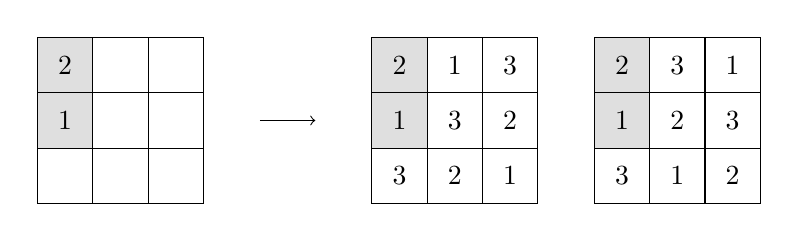
\begin{tikzpicture}[x=2em, y=2em]

        \tikzset{
          ls/.pic={
            \draw
            (0,0) rectangle (3,3)
            foreach \i in {1,2} { (0,\i) -- +(3,0) (\i,0) -- +(0,3) };

            \foreach \i/\j/\n in {0/2/2,0/1/1} {
              \fill[opacity=1/8] (\i,\j) rectangle +(1,1);
              \node at (\i+1/2,\j+1/2) {\(\n\)};
            };
          },
          lss/.pic={
            \pic{ls};
            \node at (1/2,1/2) {\(3\)};
            \foreach \i in {0,1,2} {
              \pgfmathtruncatemacro\m{Mod(\i+#1-1,3)+1}
              \pgfmathtruncatemacro\n{Mod(\i-#1-1,3)+1}
              \node at (1+1/2,\i+1/2) {\(\m\)};
              \node at (2+1/2,\i+1/2) {\(\n\)};
            }
          },
        }

        \matrix[column sep=2em] {
          \pic{ls}; & \draw[->] (0,3/2) -- +(1,0); &
          \pic{lss=-1}; & \pic{lss=1}; \\
        };

      \end{tikzpicture}

      \caption{A \(3×3\) Latin Square instance and its two possible
      completions.}

      \label{fig:background.latin-square-example}

    \end{center}
  \end{figure}

\item[\Problem{Graph Coloring}] Given a positive integer \(k\), and a graph
  with \(n>k\) vertices, some of which are assigned a number (a.k.a. ``color'')
  in \(\Set{1,\dotsc,k}\), is it possible to assign numbers to the remaining
  cells so that no neighboring vertices receive the same assignment?

  \begin{figure}[H]
    \begin{center}
      \begin{tikzpicture}


      \end{tikzpicture}
    \end{center}
  \end{figure}


  TODO diagram illustrations.  also i wish i could think of simpler-to-state
  examples with easy reductions, but nothing comes to mind, so this is the best
  i've got for now.

\end{description}

Is one of these problems ``easier'' than the other?  In a sense, yes: the
\Problem{Latin Square} problem is just a special case of the \Problem{Graph
Coloring} problem, where the vertices are arranged into a square grid, and all
vertices in the same row or column neighbor each other.

\begin{figure}[H]
  \begin{center}
    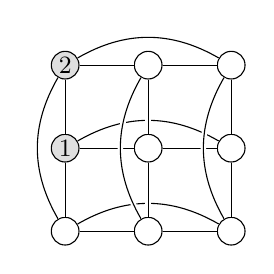
\begin{tikzpicture}[x=3em, y=3em]

      \tikzset{
        vert/.style={circle, draw, minimum size=1em, inner sep=0pt, font=\small},
        pre/.style={vert, fill, fill opacity=1/8, text opacity=1},
        edge/.style={preaction={draw=white, line width=2pt}},
      }

      \node[pre](02) at (0,2) {\(2\)};
      \node[pre](01) at (0,1) {\(1\)};
      \coordinate[vert](00) at (0,0){};

      \foreach \i in {1,2} { \foreach \j in {0,1,2} {
          \coordinate[vert](\i\j) at (\i,\j);
      } };

      \draw[edge] foreach \i in {0,1,2} { (0\i) to[bend left] (2\i) };
      \draw[edge] foreach \i in {0,1,2} { (\i0)--(\i1)--(\i2) (0\i)--(1\i)--(2\i) };
      \draw[edge] foreach \i in {0,1,2} { (\i0) to[bend left] (\i2) };

    \end{tikzpicture}

    \caption{The Latin Square from \cref{fig:background.latin-square-example},
    represented as a graph.}

  \end{center}
\end{figure}

More precisely, this argument describes a way to convert any \Problem{Latin
Square} instance (a partially-filled \(n×n\) grid) into a \Problem{Graph
Coloring} instance (a partially-colored graph with \(n²\) vertices) with the
same yes/no answer.  Formally, we call this conversion a \Term{reduction}:

\begin{definition}{reductions}{}

  Let \(Π₁\) and \(Π₂\) be decision problems.  A \Term{reduction} from \(Π₁\)
  to \(Π₂\) is an algorithm \(R\colon\Set{0,1}^*→\Set{0,1}^*\) such that, for
  each \(X∈\Set{0,1}^*\), \(X∈Π₁\) if and only if \(R(X)∈Π₂\).

  In other words, \(R\) converts problem-inputs (a.k.a. \emph{instances}) of
  \(Π₁\) to problems-inputs of \(Π₂\) such that the yes/no answers on the
  original and converted inputs exactly match.

  %\begin{aside}
  %  %This definition is sometimes called \emph{Karp reductions} or
  %  %\emph{many-one reductions}, in order to distinguish it from other notions
  %  %of reduction such as \emph{Turing/Cook reductions} and \emph{truth-table
  %  %reductions}, which are related but different.

  %  %For our purposes, Karp reductions are the simplest to describe and
  %\end{aside}

\end{definition}

Revisiting the above example, the existence of a reduction from \Problem{Latin
Square} to \Problem{Graph Coloring} captures the idea that \Problem{Latin
Square} is easier than \Problem{Graph Coloring} in the following sense.
Suppose that we already know how to solve \Problem{Graph Coloring}.  Then, we
automatically also know how to solve \Problem{Latin Square}: given an arbitrary
\Problem{Latin Square} input, apply the reduction to convert it into a
\Problem{Graph Coloring} input, feed that input into the known \Problem{Graph
Coloring} solver, then directly return its answer.

However, in order to authentically capture the idea of \emph{easiness}, we must
also account for computation time.  Namely, we stipulate that the reduction
itself must be efficient---formally, that it runs in polynomial time.

\begin{definition}{polynomial-time reducibility}{}

  Let \(Π₁\) and \(Π₂\) be decision problems.  We say \(Π₁\) is
  \Term{polynomial-time-reducible} to \(Π₂\), which we denote as
  \[
    Π₁≤Π₂,
  \]
  if there exists a reduction from \(Π₁\) to \(Π₂\) that runs in polynomial
  time.  (The \(≤\) notation evokes the intuition that \(Π₁\) is easier than,
  or \emph{at most as hard as}, \(Π₂\).)

\end{definition}

Finally, we introduce some terminology to describe how one problem compares to
a \emph{class} of problems:

\begin{definition}{hardness and completeness}{}

  Let \(Π\) be a decision problem, and let \(\C\) be a class of decision
  problems.

  We say \(Π\) is \Term{hard} for \(\C\), or \Term{\C-hard}, if every
  problem in \C{} is polynomial-time-reducible to \(Π\).

  We say \(Π\) is \Term{complete} for \C, or \Term{\C-complete}, if \(Π\) is
  \C-hard and \(Π∈\C\).

  \begin{aside}
    Following the intuition that reducibility (\(≤\)) defines a (partial)
    ordering of problems by difficulty, \C-hard problems are just those that
    are (non-strictly) harder than all problems in \C, and \C-complete problems
    are just the \emph{maximal/hardest} problems within \C.
  \end{aside}

\end{definition}

Complete problems are especially useful, first and foremost, because they are
tangible.  They have accessible, interesting, and often real-world-applicable
examples that help us understand complexity classes in concrete, intuitive
terms, rather than pure abstractions.  At the same time, complete problems are
also very general.  As \emph{tight} difficulty upper bounds of a complexity
class, they are perfect characterizations of these classes; determining the
exact difficulty of a complete problem automatically essentially determines the
difficulty of the entire complexity class.

%By studying complete problems for a spectrum of complexity classes, we gain
%wholesale but vivid insight

% TODO i feel like i want to have a conclusion punchline here

%Now, it is time to study a collection of complete problems
%
%satisfiability games.



%\section{Puzzles, non-determinism, and \NP}

%Consider the following problem.
%\begin{itemize}
%  \item Given a graph \(Γ\) and a positive integer \(k\), does \(Γ\) contain a
%    clique of size \(k\)?
%\end{itemize}


%\section{Hard problems and completeness}

%Notationally, we say \(X\) is \emph{in} the problem \(L\), or \(X\in L\), if
%the answer is yes; otherwise, we say \(X\notin L\).
%
%An example of a decision problem is the graph reachability problem:
%\begin{definition}[\Problem{reachability}]%
%  Given a graph with \(n\) vertices \(v_1, \dots, v_n\), does there exist a
%  path connecting \(v_1\) to \(v_n\)?
%\end{definition}
%This problem may be solved using simple graph-search algorithms such as
%Breadth-First/Depth-First Search, whose asymptotic running time is \(\O(n)\)
%---that is, bounded by a linear function of \(n\).  As such, this problem is
%considered relatively ``easy'' to solve.
%
%More generally, \Problem{reachability} belongs to the class of decision
%problems known as \P:
%\begin{definition}[\P]%
%  The class of decision problems whose solution runtime is bounded by a
%  polynomial function of the input length.
%\end{definition}
%We consider problems in \P{} to be ``easy''---at least, from the standpoint of
%computational complexity.
%
%Another example of a decision problem is the Hamiltonian path problem:
%\begin{definition}[\Problem{hamiltonian-path}]%
%  \label{def:hamiltonian-path} Given a graph with \(n\) vertices, does it
%  contain a Hamiltonian path (i.e., a path that visits each vertex exactly
%  once)?
%\end{definition}
%This problem is not known to be in \P.  In fact, the best known algorithms
%solving \Problem{hamiltonian-path} are essentially brute-force guess-and-check:
%\emph{guess} a possible Hamiltonian path (e.g., by writing down some
%permutation of the vertices), then \emph{check} that it is valid (e.g., that
%each pair of adjacent vertices in the guessed path are actually connected by an
%edge in the graph).  In the worst case, if our guesses are really unlucky, we
%may have to repeat up to \(n!\) iterations, which is definitely not polynomial.
%However, setting aside the cost associated with brute-forcing guesses, note
%that individual \emph{checking} steps \emph{do} run in polynomial time.
%Problems like this, which are solvable via guess-and-check, where the ``check''
%problem is in \P, belong to a class of problems known as \NP:
%\begin{definition}[\NP]%
%  \label{def:np} A decision problem \(L\) is in \NP{} if\dots
%  \begin{nested}
%    there exists a corresponding decision problem \(L'\in\P\) (intuitively: the
%    ``check'' problem) and a polynomial \(p\) such that\dots
%    \begin{nested}
%      for all input strings \(x\)\dots
%      \begin{nested}
%        \(x \in \NP\) if and only if\dots
%        \begin{nested}
%          there exists a ``guess'' \(g\) with length \(\Abs g \le p(\Abs x)\)
%          such that \((x, g) \in L'\) (intuitively: \(g\) passes the
%          ``check'').
%        \end{nested}
%      \end{nested}
%    \end{nested}
%  \end{nested}
%
%  Note that the \(\Abs g \le p(\Abs x)\) requirement is present in order to
%  ensure that the guesses are not so obscenely long as to abuse the idea of
%  ``efficient'' checking.  This requirement is not central to understanding the
%  definition of \NP{} but is nevertheless an important technical subtlety.
%\end{definition}
%
%The infamous \P-vs-\NP{} open question asks: is \NP{} truly more difficult than
%\P?  Does there exist some problem in \NP{} that definitively cannot be solved
%within polynomial time?  I, a baby undergraduate, am not in the business of
%answering that question.
%
%As such, the best we can do to determine the difficulty of a given problem is
%to compare them to other problems, deriving a \emph{relative} ordering telling
%us which problems are easier/harder than other ones.  To this end, we must
%define what easier/harder means---intuitively, we think of a problem \(L_1\) as
%easier than another problem \(L_2\) if knowing how to solve \(L_2\)
%automatically also tells us how to solve \(L_1\), with minimal
%(polynomially-bounded) overhead.  More precisely:
%\begin{definition}[reductions]
%  \label{def:reduction}
%  Let \(L_1\) and \(L_2\) be decision problems.  We say \(L_1\) is
%  \emph{reducible to} \(L_2\), or that \(L_1\) is \emph{at least as easy as}
%  \(L_2\)'', denoted \(L_1 \le L_2\), if\dots
%  \begin{nested}
%    there exists a function \(f\), called a \emph{reduction}, converting input
%    strings for \(L_1\) to inputs for \(L_2\), such that \(f\) is computable
%    within polynomial time, and\dots
%    \begin{nested}
%      for any input \(x_1\)\dots
%      \begin{nested}
%        \(x_1 \in L_1\) if and only if \(x_2 \in L_2\).
%      \end{nested}
%    \end{nested}
%  \end{nested}
%
%  Note that this definition of reductions is slightly different than the one
%  given in \textcite{papadimitriou.cc}, whose requirement on \(f\) is that it
%  is computable in \emph{logarithmic-space} rather than polynomial-time.
%  However, for the purposes of this project, the distinction between the two is
%  unimportant.
%\end{definition}
%
%This notion of comparison also gives us a good way of comparing problems to
%entire classes:
%\begin{definition}[hardness and completeness]%
%  \label{def:hard-complete}
%  Let \(\mathbfit C\) be a complexity class.
%  \begin{itemize}[nosep]
%    \item A problem \(L\) is \emph{hard for \(\mathbfit C\)}, or
%      \emph{\(\mathbfit C\)-hard}, if \(L\ge K\) for every \(K\in\mathbfit C\).
%    \item A problem \(L\) is \emph{complete for \(\mathbfit C\)}, or
%      \emph{\(\mathbfit C\)-complete}, if \(L\) is \(\mathbfit C\)-hard
%      \emph{and} \(L\in\mathbfit C\).
%  \end{itemize}
%\end{definition}
%
%In particular, \emph{complete} problems for a class \(\mathbfit C\) are at
%least as hard as everything else in \(\mathbfit C\) and simultaneously
%themselves \emph{in} \(\mathbfit C\).  In this sense, for any complexity class,
%its complete problems are its \emph{hardest} problems, giving us an effective,
%``exact'' characterization of the class in terms of its problems.
%
%This approach to characterizing complexity classes is the driving motivation
%behind our exploration of puzzles and games.
%
%%\todo[inline]{unfinished.  formalism of turing machines, decision problems,
%%  oracles \& the definition of polynomial hierarchy, proofs of completeness of
%%  SAT \& QSAT for classes in the polynomial hierarchy.  I imagine this stuff
%%  will be needed in the final thesis; is it needed also for the midyear
%%report?}
%%
%%\begin{definition}[decision problem/language]%
%%  A \textbf{decision problem} is a yes/no question posed on binary input
%%  strings, or problem \textbf{instances}.  As such, we may think of a decision
%%  problem as a mapping
%%  \[
%%    L \colon \Set{0, 1}^* \to \Set{\text{yes}, \text{no}}.
%%  \]
%%
%%  More commonly, we associate a problem with its ``yes'' instances, the set of
%%  which is a \textbf{language}:
%%  \[
%%    L(L) = \SetBuilder* {x \in \Set{0, 1}^*} {L(x) = \text{yes}}.
%%  \]
%%  Here, for clarity, we are distinguishing notationally between \(L\) and
%%  \(L(L)\), but in general we conflate the two notions and refer to both as
%%  the problem \(L\).
%%\end{definition}
%%
%%\begin{definition}[\NP]
%%  \NP{} is the class of problems solvable by a \emph{non-deterministic} Turing
%%  machine in \emph{polynomial time}.
%%\end{definition}
%%
%%
%%
%%

\chapter{A primer on boolean logic}
\label{ch:boolean}

Mathematical logic is founded on true-or-false statements---statements such as:
\begin{itemize}[nosep]
  \item property \(A\) is \emph{true} when condition \(B\) is \emph{false},
  \item property \(X\) is \emph{true} when both condition \(Y\) and condition
    \(Z\) are \emph{true},
\end{itemize}
and so on.  Boolean logic refers to the algebra of how \emph{truthiness} and
\emph{falsiness} combine and transform under various logical operations.

It is no surprise, given the foundational role of booleans in mathematical
logic, that they also underpin all computational logic. For instance, all
modern computer architectures deal with data encoded in binary \(0\)s
(\emph{false}) and \(1\)s (\emph{true}).  Furthermore, it follows that
everything we conceive of as ``computer'' can be represented as boolean
circuits---because, essentially, they literally are boolean circuits.

% TODO: this observation underlies importance of boolean puzzles/games, etc.; how this comes up later, blah

In this short chapter, we outline some basic definitions and facts about
boolean-logical operations and circuits, along with some notational conventions
used throughout the rest of this thesis.

\begin{definition}{basic boolean operations: \NOT, \AND, \OR}{}

  \begin{description}

  \item[\NOT] takes one input and outputs its opposite value.  In
    boolean-algebraic expressions, we denote \NOT{} with the symbol \(¬\).
    \[
      ¬\colon\Set{\True,\False}→\Set{\True,\False} \qquad
      ¬x =
      \begin{cases}
        \True & x=\False \\
        \False & x=\True
      \end{cases}.
    \]
    The \NOT{} operation is also commonly known as \Term{negation}.

  \item[\AND] takes two inputs and outputs \True{} if and only if \emph{both}
    of its inputs are \True.  We denote \AND{} with the symbol \(∧\).
    \[
      ∧\colon\Set{\True,\False}²→\Set{\True,\False} \qquad
      x∧y =
      \begin{cases}
        \True & x=y=\True \\
        \False & \text{otherwise}
      \end{cases}.
    \]

    For convenience, we sometimes omit the \(∧\) and simply denote \AND{} by
    concatenating the operands, as in \(xy\) instead of \(x∧y\).  (This
    notation looks like multiplication because it is: if we represent boolean
    values with \(\Set{1,0}\) instead of \(\Set{\True,\False}\), then
    \(x∧y=x⋅y\).)

    \AND{} is also known as the \Term{conjunction} operation.

  \item[\OR] takes two inputs and outputs \True{} if \emph{at least one} of its
    inputs are \True.  We denote \OR{} with the symbol \(∨\).
    \[
      ∨\colon\Set{\True,\False}²→\Set{\True,\False} \qquad
      x∨y =
      \begin{cases}
        \False & x=y=\False \\
        \True & \text{otherwise}
      \end{cases}.
    \]

    \OR{} is also known as the \Term{disjunction} operation.

  \end{description}

  Notationally, \(∧\) takes higher precedence than \(∨\).  For instance, we
  interpret \(x∨y∧z=x∨yz=x∨(y∧z)\), and so on.

  \begin{aside}
    I personally find the \(∧\) and \(∨\) symbols for \AND{} and \OR{} quite
    easy to mix up with each other.  Here's a mnemonic that helps me remember
    which is which:
    \begin{itemize}[nosep]
      \item \(∧\) looks like the \(\mathrm{\scriptstyle A}\) in \AND, so \(∧\)
        means \AND…
      \item \(∨\) is the other one.
    \end{itemize}
  \end{aside}

\end{definition}

\section{Algebraic properties of \(¬,∧,∨\)}

What algebraic behaviors do \(¬\), \(∧\), and \(∨\) exhibit?

\paragraph{Commutativity \& associativity} It follows straightforwardly from
their definitions that they are both commutative and associative.  In general,
for any \(x₁,x₂,\dotsc,xₙ∈\Set{\True,\False}\),
\begin{align*}
  ⋀ᵢ₌₁ⁿ xᵢ &= x₁∧\dotsb∧xₙ = \text{\True{} if and only if \emph{every one} of
  \(x₁,\dotsc,xₙ\) is \True}, \\
  ⋁ᵢ₌₁ⁿ xᵢ &= x₁∨\dotsb∨xₙ = \text{\True{} if and only if \emph{at least one} of \(x₁,\dotsc,xₙ\) is \True}.
\end{align*}

\paragraph{Distributivity} Another interesting, sometimes useful, property of
\(∧\) and \(∨\) is that they distribute over each other.  For all
\(x,y,z∈\Set{\True,\False}\),
\[
  x∧(y∨z) = (x∧y)∨(x∧z), \qquad
  x∨(y∧z) = (x∨y)∧(x∨z).
\]

%\begin{aside}
%  Here are two intuitive examples demonstrating this distributivity.
%
%  \begin{itemize}
%
%    \item Consider the statement, ``Alex and (either Blake or Charlie) ate
%      pizza'', encoded as the boolean statement \(A(B∨C)\).  What are the
%      possible combinations of pizza-eaters?
%
%      The answer: either Alex and Blake, or Alex and Charlie.  That is,
%      \[
%        A(B∨C) = AB∨AC.
%      \]
%
%    \item Consider the statement, ``either Alex is a vegetarian, or Charlie and
%      Blake both are''.
%
%  \end{itemize}
%
%
%\end{aside}

%\section{Computing arbitrary boolean functions}
%
%Any boolean function can be expressed in terms of the three operators
%\(¬,∧,∨\).


\subsection{DeMorgan's identities}

Consider the statement, ``\(x,y\) are both \False''.  There are two equivalent
ways to express this statement algebraically:
\begin{itemize}[nosep]
  \item \(x\) is \False, and \(y\) is \False: \(¬x∧¬y\).
  \item Neither of \(x,y\) is \True: \(¬(x∨y)\).
\end{itemize}
The equivalence of these two expressions gives rise to an identity: for all
\(x,y∈\Set{\True,\False}\),
\[
  ¬x∧¬y = ¬(x∨y).
\]

Similarly, the statement ``at least one of \(x,y\) are \False'' can be
expressed in two ways,
\begin{itemize}[nosep]
  \item \(x\) is \False, or \(y\) is \False: \(¬x∨¬y\).
  \item \(x,y\) are not both simultaneously \True: \(¬(x∧y)\).
\end{itemize}
This equivalence gives rise to a dual identity,
\[
  ¬x∨¬y = ¬(x∧y).
\]

A particularly useful consequence of these DeMorgan identities is that having
all three logical operations is \emph{redundant}.  We didn't need to define all
three as the basic building-block operations; having only \NOT/\OR{} or
\NOT/\AND{} suffices, since the third operation can simply be constructed in
terms of the other two:
\[
  x∧y = ¬(¬x∨¬y), \qquad
  x∨y = ¬(¬x∧¬y).
\]

We make use of this convenience later in chapters TODO, when we try to embed
boolean logic within other ``computer-like'' systems such as graph colorings
and exact set coverings, etc.

% The usefulness of this redundancy
%
% that if we were trying to simulate boolean logic within some other system (we
% explore this idea later in more detail when we explore reductions from boolean
% circuits in chapters TODO),
%
% universality of not/and and not/or

% TODO miscellaneous identities?


% TODO boolean logical operations can compute arbitrary boolean functions

\section{Boolean circuits}

Boolean \emph{expressions} such as \(¬x∧y\) are one way to specify computations
on boolean variables.  \emph{Circuits} generalize expressions by essentially
chaining together a pipeline of expressions, allowing intermediate results at
each stage to be saved and reused.  To illustrate, consider the following
example expression:
\[
  ϕ(x₁,x₂,y₁,y₂,z₁,z₂)
  = (x₁∨x₂)(y₁∨y₂) ∨ (y₁∨y₂)(z₁∨z₂) ∨ (z₁∨z₂)(x₁∨x₂).
\]
Notice that each \((□₁∨□₂)\) term appears twice in the expression, making the
expression inefficient to evaluate (each repeated term would be unnecessarily
recomputed), not to mention cumbersome to specify.  A more elegant way to
specify this computation is to store and reuse the intermediate terms:
\begin{align*}
  X &= x₁∨x₂, \\
  Y &= y₁∨y₂, \\
  Z &= z₁∨z₂, \\
  ϕ &= XY∨YZ∨ZX.
\end{align*}
This chain of assignments may be visualized as a sort of data-processing
``pipeline'', with intermediate inputs and outputs at each stage:

{

  \tikzset{
    input/.style={
      circle,
      fill,
      inner sep=0pt,
      minimum size=3pt,
    },
    gate/.style={
      draw,
      rounded corners=1em/8,
    },
    pipe/.style={
      rounded corners=1em/2,
      to path={
        (\tikztostart)
        -- ($ (\tikztostart -| \tikztotarget)!3em!(\tikztostart) $)
        %-- ($ (\tikztotarget)!1em!(\tikztostart |- \tikztotarget) $)
        -- (\tikztotarget)
      },
      ->,
    },
    over/.style={
      preaction={
        draw=white,
        line width=2pt,
      },
    },
    gates/.style={
      row sep=2em, column sep=6em, matrix of math nodes, nodes=gate,
    },
    wires/.pic={

      \foreach \var in {x,y,z} {
        \coordinate (\var1) at ($ (\var.west) + (-4em,2em/3) $);
        \coordinate (\var2) at ($ (\var.west) + (-4em,-2em/3) $);
        \draw[pipe] (\var1) node[left]{\(\var₁\)} to ($ (\var.north west)!2/3!(\var.west) $);
        \draw[pipe] (\var2) node[left]{\(\var₂\)} to ($ (\var.south west)!2/3!(\var.west) $);
        \node[above right] at (\var.east) {\(\MakeUppercase{\var}=\var₁∨\var₂\)};
      }
      \draw[pipe] (y.east) to (xy.south west);
      %\draw[pipe] ($ (yz.west)!3em!(y.east) $) to ($ (xy.west)!1/2!(xy.south west) $);
      \draw[pipe] (y.east) to (yz.west);
      %\draw[pipe] ($ (zx.west)!3em!(z.east) $) to ($ (yz.west)!1/2!(yz.south west) $);
      \draw[pipe] (z.east) to (yz.south west);
      \draw[pipe] (z.east) to (zx.west);
      %\draw[pipe] ($ (zx.west)!3em!(z.east) $) to ($ (yz.west)!1/2!(yz.south west) $);
      \draw[pipe, over] (x.east) to (zx.north west);
      \draw[pipe] (x.east) to (xy.west);

      \foreach \gate in {xy,yz,zx} {
        \node[above right] at (\gate.east) {\(\MakeUppercase{\gate}\)};
      }

    },
  }

  \begin{center}
    \begin{tikzpicture}
      \matrix[gates, ampersand replacement=\&]{
        |(x)|∨ \&[2em] |(xy)|∧ \\
        |(y)|∨ \& |(yz)|∧ \& |(out)|∨ \\
        |(z)|∨ \& |(zx)|∧ \\
      };

      \pic{wires};
      \draw[pipe] (xy.east) to (out.north west);
      \draw[pipe] (yz.east) to (out.west);
      \draw[pipe] (zx.east) to (out.south west);
      \draw[->] (out.east) -- +(2em,0) node[right]{\(ϕ=XY∨YZ∨ZX\)};
    \end{tikzpicture}
  \end{center}

  This is \emph{essentially} a boolean circuit.  More precisely, in a boolean
  circuit, each variable (e.g., \(x₂\) or \(Y\)) is represented as a \emph{wire}
  carrying a boolean value, and each ``stage'' of computation, called a
  \emph{logic gate}, computes an individual boolean operation.

  For simplicity's sake, we also require that each \AND/\OR{} gate operates on
  exactly two inputs.  Thus the last \OR{} operation \(XY∨YZ∨ZX\) should
  actually be associatively grouped as \((XY∨YZ)∨ZX\).  The corrected circuit
  is shown below:

  \begin{center}
    \begin{tikzpicture}
      \matrix[gates, ampersand replacement=\&]{
        |(x)|∨ \&[2em] |(xy)|∧ \\
        |(y)|∨ \& |(yz)|∧ \&\& |(or')|∨ \\
        |(z)|∨ \& |(zx)|∧ \\
      };

      \node[gate](or) at ($ (xy)!1/2!(or') $){\(∨\)};

      \pic{wires};
      \draw[pipe] (xy.east) to ($ (or.west)!1/3!(or.north west) $);
      \draw[pipe] (yz.east) to ($ (or.west)!1/3!(or.south west) $);
      \draw[pipe] (or.east) to ($ (or'.west)!1/3!(or'.north west) $);
      \draw[pipe] (zx.east) to ($ (or'.west)!1/3!(or'.south west) $);
      \node[above right] at (or.east) {\(XY∨YZ\)};
      \draw[->] (or'.east) -- +(2em,0) node[right]{\(ϕ=(XY∨YZ)∨ZX\)};

    \end{tikzpicture}
  \end{center}

}

%Lastly, we use the algebraic symbols \(∨,∧\) to denote the logic gates in the
%circuit diagram above

Below, we give a precise definition of boolean circuits and introduce some
relevant terminology.

\begin{definition}{boolean circuits, logic gates}{}

  A \Term{boolean circuit}

  TODO precise definition

\end{definition}


%We give a precise definition of
%
%\begin{definition}{boolean circuits}{}
%
%  % TODO consider using switches and lightbulbs in formalism
%
%  A \Term{circuit} consists of a network of such wires and logic gates, with
%  the following requirements for well-defined-ness:
%  \begin{itemize}
%    \item Some wires are marked as circuit-level \Term{inputs}.  These wires
%      may not be the output wire of any gate within the circuit.
%    \item Every wire that isn't a circuit-level input must be the output wire
%      of exactly one logic gate.
%    \item There must be no (directed) cycles in the circuit.  That is, there
%      must not exist gates \(g₁,\dotsc,gₖ\) such that the output of \(g₁\) is
%      an input to \(g₂\), the output of \(g₂\) an input to \(g₃\), …, and the
%      output of \(gₖ\) an input to \(g₁\).
%    \item Finally, there is exactly one wire marked the \Term{output} of the
%      circuit.
%  \end{itemize}
%  Under these requirements, each combination of boolean values assigned to the
%  circuit-level input wires, uniquely determines the circuit-level output's
%  value. Therefore, a circuit with \(n\) inputs defines a function
%  \(\Set{\False,\True}ⁿ→\Set{\False,\True}\).
%
%  To simplify notation, we refer to each circuit and its boolean function by
%  the same name.  That is, if \(C\) refers to a circuit, we denote by
%  \(C(x₁,\dotsc,xₙ)\) the output computed by \(C\) on input values
%  \(x₁,\dotsc,xₙ\).  Occasionally, if we need to disambiguate between a circuit
%  and its function, we denote the circuit \(C\) and its function \(ϕ_C\).
%
%\end{definition}


\chapter{Boolean circuit puzzles and games}
\label{ch:circuit}

In this chapter, we begin to explore landscape of puzzle-and-game complexity
classes---specifically, the \emph{polynomial hierarchy}---through a series of
games played on boolean circuits.

\section{The \Problem{Circuit Value} problem, and \texorpdfstring{\(\ComplexityClass{P}\)}{𝐏}}

To set the stage, we start with a relatively ``easy'' problem, known as the
\Problem{Circuit Value} problem, or \Problem{CircVal} for short:

%\begin{definition}{\(\Problem{Circuit Value}=\Problem{CircVal}\)}{}
%
%  Let \(C\) be a given boolean circuit with all input wires/variables
%  specified. What is the final output value of \(C\)? As a decision problem:
%  \(C∈\Problem{Circuit Value}\) if it outputs \True, and \(C∉\Problem{Circuit
%  Value}\) if it outputs \False.
%
%\end{definition}

\begin{problem}[lefthand ratio=.5]{\Problem{Circuit Value} / \CircVal}{circ-val}
  \begin{description}[nosep]
    \item[Given:] a boolean circuit with all inputs specified
    \item[Return whether:] the circuit outputs \True
  \end{description}
  %

  %Given a boolean circuit with all inputs specified, compute its output. Return
  %\emph{yes} if the output is \True.
%
%  \tcblower
%  \CircVal = \SetBuilder{\text{circuit \(C\)}}{C()=\True}
\end{problem}

It is well-known that \(\CircVal∈\P\) (i.e., it is actually ``easy'').  We give
one version of a proof below.

\begin{theorem}{\(\CircVal∈\P\)}{}

  \CircVal{} is solvable in polynomial time.

\end{theorem}

\begin{proof}
  We give a polynomial-time algorithm solving \Problem{Circuit Value} below.
  (Note that this is not the most efficient algorithm doing so; we choose it
  here only for its simplicity.)

  \begin{algorithm}{a polynomial-time \CircVal{} solver}{}
    \begin{algorithmic}
      \Given{\(C\), a boolean circuit with all inputs fully specified}
      \LComment{Call a wire \emph{finished} if it has been assigned a boolean
        value. Initially, all the input wires are finished, since their values
      were given, and all intermediate and output wires are unfinished.}%
      \While{final output wire is not finished}%
      \ForEach{unfinished logic gate \(g\) in \(C\)}%
      \If{all input wires of \(g\) are finished}%
      \State{compute and assign the output value of \(g\) to its output wire}%
      \EndIf%
      \EndFor%
      \EndWhile%
      \State \Return value assigned to final output wire%
    \end{algorithmic}
  \end{algorithm}

  We argue that this algorithm terminates in polynomial time.  On each
  iteration of the ``while'' loop, at least one logic gate is guaranteed to
  have all of its inputs done, since there are no cyclic dependencies in the
  circuit.  Thus each iteration of the ``while'' loop finishes at least one
  additional wire.  Therefore, the number of ``while'' iterations is at most
  the number of wires in the circuit, and the work done within each iteration
  is also polynomial with respect to the size of the circuit, so the overall
  algorithm terminates in polynomial time.
\end{proof}

To kickstart the puzzles-and-games perspective, we think of \Problem{Circuit
Value}---and actually, every problem in \P---as a game with \(0\) turns: the
player does nothing, and an (efficient) algorithm automatically decides whether
the player wins or loses.

This seems like a silly (arguably boring) idea.  But, as we see in the next few
sections, this approach allows us to generalize \Problem{Circuit Value} into
very powerful puzzles and games.

\section{The \Problem{Circuit Satisfiability} puzzle, and \NP}

By \emph{puzzle}, we really mean \(1\)-turn games: games in which a player
makes a sequence of ``moves'' on a given ``game board'', and an (efficient)
algorithm then determines whether the player's moves constitute a win.
Formulated as decision problems, the computational puzzle is the yes/no
question:
\begin{center}
  Does the player have a winning strategy?
\end{center}

For example, consider a puzzle-ification of \Problem{CircVal}, where the
circuit's inputs are no longer specified but rather chosen by the player (this
is the ``move'' made by the player).  Recall that the player wins if the
circuit's output is \True.  Thus, when we allow the player to choose inputs, a
winning strategy means a combination of inputs causing the circuit to output
\True.  The decision problem asking whether such a winning move exists is
called \Problem{Circuit Satisfiability}, or \Problem{CircSat} for short:

%\begin{definition}{\(\Problem{Circuit Satisfiability}=\Problem{CircSat}\)}{}
%
%  Let \(C\), a boolean circuit, be given. Does there exist a combination of
%  boolean input values to \(C\) causing it to output \True?
%
%\end{definition}

\begin{problem}{\Problem{Circuit Satisfiability} / \CircSat}{circsat}

  Given a boolean circuit \(C\), determine whether there exists some assignment
  to its inputs causing its output to be set to \True.  Such an assignment is
  called a \Term{satisfying assignment of \(C\)}.
%
%  \tcblower
%  \CircSat = \SetBuilder{\text{circuit \(C\) with \(n\) inputs}}{∃X∈\TF[n]\Q C(X)=\True}
\end{problem}

Briefly: how (computationally) difficult is \Problem{CircSat}?  As it turns
out, nobody knows for sure, but it seems \emph{quite} difficult.  Loosely
speaking, all known algorithms for solving \Problem{CircSat} amount to brute
force with optimizations that enhance performance on ``practical'', real-world
inputs but do not save them from performing poorly in the worst case.
Tentatively, then, most computer scientists suspect that
\(\Problem{CircSat}∉\P\)---i.e., there is no polynomial-time solution for
\Problem{CircSat}.

TODO: here's a survey to cite on on pnp opinion:
\url{https://dl.acm.org/doi/10.1145/564585.564599}.  cite it correctly later.
% https://www.researchgate.net/publication/292393040_The_PNP_poll

% TODO maybe cite an up-to-date result about how good the bound is, but whatever

% useful citation about best-known SAT bounds: https://cstheory.stackexchange.com/questions/1060/best-upper-bounds-on-sat

% https://www.sciencedirect.com/science/article/pii/S0304397501001748?via%3Dihub
% 3sat solvable in 1.5^n?



Anyway, back to puzzles.  \Problem{CircSat} is one example of how a \(0\)-turn
game such as \Problem{CircVal} may be generalized into a \(1\)-turn game---a
puzzle.  How can we do this in general, for arbitrary games?

In the example of \Problem{CircSat}, we do this by making the player supplement
the input to the the \(0\)-turn analog, \Problem{CircVal}.  This approach is
readily generalized.  Given some input \(X\) (the ``game board''), construct a
\(1\)-turn game in which the player specifies a supplementary input \(Y\);
victory is decided by whether the pair of inputs \((X,Y)\) meets the \(0\)-turn
winning condition, which should be an efficiently-computable condition---a
problem in \P.  As before, the decision problem asks whether the player can win:
does there exist \(Y\) such that \((X,Y)\) meets the winning condition?

The complexity class of all \(1\)-turn game problems constructed in this manner
is called \NP.  Before we give the formal definition of \NP, we need to
introduce one more technical detail.  In the discussion above, call \(Π\) the
\(0\)-turn winning condition problem.  We said above that \(Π\) should be
computable in polynomial-time.  More precisely, we want it to be computable in
polynomial-time with respect to the size of the \emph{game board} \(X\).
However, the input string to the \(Π\) isn't just \(X\) but the pair \((X,Y)\),
so simply requiring \(Π∈\P\) is insufficient: polynomial with respect to the
size of \((X,Y)\) does not imply polynomial with respect to the size of \(X\)
(\(Y\) could be arbitrarily long).  To fix this disparity, we additionally
require that the player's input scales controlledly with the game board: the
size of \(Y\) must be polynomially-bounded by the size of \(X\).

%This requirement guarantees that
%\(Y\) does not unduly distort the input size, and any polynomial function on the
%size of \((X,Y)\) is also polynomial with respect to the size of \(X\).  We call
%problems with this constraint \emph{polynomially balanced}.
%
%\begin{definition}{polynomially balanced}{balance}
%
%  Let \(Π⊆\Set{0,1}^*×\Set{0,1}^*\) be a decision problem whose inputs are
%  \emph{pairs} of strings.  We say \(Π\) is \Term{polynomially balanced} if
%  there exists a polynomial function \(p\) such that, for every \((X,Y)∈Π\),
%  \[
%    \Abs Y≤p(\Abs X).
%  \]
%
%\end{definition}

We are now ready to give the full definition of \NP{} (the class of all
\(1\)-turn games).

\begin{definition}{\NP}{np}

  \NP{} is the class of decision problems \(Π\) such that
  \begin{nest}
    there exists a \(Π'∈\P\) (the \(0\)-turn winning condition) and a polynomial
    \(p\) such that
    \begin{nest}
      for each input \(X∈\Strings\) (the game board)
      \begin{nest}
        \(X∈Π\) (the player can guarantee a win) if and only if
        \begin{nest}
          there exists \(Y∈\Strings\) (the player's move) such that \(\Abs
          Y≤p(\Abs X)\), and
          \begin{nest}
            \((X,Y)∈Π'\) (the move meets the winning condition).
          \end{nest}
        \end{nest}
      \end{nest}
    \end{nest}
  \end{nest}

\end{definition}

Notice the inductive relationship between \P{} and \NP.  Each problem \(Π∈\NP\)
is constructed by \emph{adding one turn} to some other problem \(Π'∈\P\).

Unsurprisingly, \CircSat{} is in \NP{} (after all, we used it as the example
problem to motivate the general definition of \NP).  To demonstrate this
inclusion formally, we show how the definition of \CircSat{} fits the definition
of \NP.

\begin{theorem}{}{}
  \(\CircSat∈\NP\).
\end{theorem}

\begin{proof}

  Let \(Π'=\CircVal\).  Specifically, think of \(Π'\) as a set of \emph{pairs}
  \((C,X)\) where \(C\) specifies the boolean circuit, and \(X\) specifies a
  input assignment to \(C\) so that \(C(X)=\True\).  The length of \(X\) always
  matches the number of input variables in \(C\), which by definition is
  polynomially bounded by the size of \(C\).

  \CircSat{} comprises exactly the set of circuits \(C\) (the game board) for
  which there exists an \(X\) (the player's move) such that
  \((C,X)∈Π'=\CircVal\).  Thus \CircSat{} fits the definition of an \NP{}
  problem.  \qedhere

\end{proof}

%Now, given a \CircSat{} instance---namely, a circuit \(C\) with \(n\)
%unspecified inputs---the player's move \(X∈\TF[n]\) augments \(C\) to form a
%new circuit \(C'=C[X]\) with \emph{no} unspecified inputs.  The player wins if
%and only if \(C'\) outputs \True; that is, if \(C'∈\CircVal\).
%\[
%  \CircSat=\SetBuilder{
%    \text{circuit \(C\) with \(n\) inputs}
%  }{
%    ∃X∈\Set{\True,\False}ⁿ\Q C[X]∈\CircVal
%  }.
%\]
%This inductive formulation of \CircSat{} shows clearly that \(\CircSat∈\NP\).
%We will also see later that the add-a-turn extension shown here can be
%generalized to construct games with many turns.

% see later in section TODO

% i wonder whether i should define projections here


%If
%\(Π\) asks the question,
%\begin{nest}
%  Does the first player have a winning strategy in a game of \(k\) turns?
%\end{nest}
%That question is answered by asking, in turn,
%\begin{nest}
%  After the first turn has been played, is the first player the guaranteed
%  winner
%\end{nest}



\subsection{\Problem{CircSat} is \NP-complete}

%We can also think of problems in \NP, or puzzles, as problems solvable by
%guess-and-check: guess a move \(Y\), and check whether it meets the winning
%condition.

What makes \CircSat{} especially interesting, compared to all the other puzzles
in \NP, is that \CircSat{} is \NP-\emph{complete}.  In other words, \CircSat{}
is the hardest of the \NP{} puzzles: any other \NP{} problem reduces to
\CircSat. This result is known as the Cook--Levin theorem:

\begin{theorem}{Cook--Levin}{cook-levin}

  \CircSat{} is \NP-complete.

\end{theorem}

A full proof of the Cook--Levin theorem would require delving into formal
technicalities about Turing Machines, which is beyond the scope of this thesis.
Instead, we give here some informal intuition about the basic idea underlying
the proof and why the Cook--Levin result makes sense.

As mentioned in \cref{ch:boolean}, any computer can be expressed in terms of
boolean circuits; in fact, modern computers literally are implemented using
boolean circuits. Therefore, the execution of any algorithm \(A\) is just a
sequence of circuit computations, one for each time-step of the algorithm. Thus
every \(1\)-turn game is really just a \emph{special case} of the
\Problem{Circuit Satisfiability} problem.

%\subsection{\True{} or \False?}
%
%In our definition of \CircSat, we say the player wins if the output of the
%circuit is set to \True.  But there is nothing special about \True---we could
%have defined the puzzle so that the player wins if the circuit outputs \False;
%the two formulations are exactly equivalent in difficulty.  Call the
%win-if-\False{} version of the puzzle \Problem{Circuit Falsifiability}:
%
%\begin{problem}{\Problem{Circuit Falsifiability}}{}
%
%  Given a boolean circuit \(C\), determine whether there exists some assignment
%  to its inputs causing its output to be set to \False.  Such an assignment is
%  called a \Term{falsifying assignment of \(C\)}.
%
%  \tcblower
%  \Problem{Circuit Falsifiability}=\SetBuilder{\text{circuit \(C\) with \(n\) inputs}}{
%    ∃X∈\TF[n]\Q C(X)=\False
%  }
%\end{problem}
%
%Note that \Problem{Circuit Falsifiability} is not the same as the
%\emph{complement} of \Problem{Circuit Satisfiability}, whose answer is ``yes''
%when the player's moves \emph{always} lead to a \False{} output:
%\begin{align*}
%  \Problem{Circuit Satisfiability} &= \SetBuilder{C}{∃X\ldotp C(X)=\True} \\
%  (\Problem{Circuit Satisfiability})\Complement &= \SetBuilder{C}{∄X\ldotp C(X)=\True}
%  = \SetBuilder{C}{∀X\ldotp C(X)=\False} \\
%  \Problem{Circuit Falsifiability} &= \SetBuilder{C}{∃X\ldotp C(X)=\False}.
%\end{align*}
%
%To see that this formulation is equivalent in difficulty to \Problem{Circuit
%Satisfiability}, we show that both problems reduce to each other.
%
%\begin{theorem}{}{}
%
%  \Problem{Circuit Satisfiability} and \Problem{Circuit Falsifiability} are
%  equivalent in difficulty.
%
%\end{theorem}
%
%\begin{proof}
%
%  Let any circuit \(C\) be given.  Compose its output with a \NOT{} gate,
%  forming a new circuit \(¬C\) whose output is always opposite that of \(C\).
%
%  Therefore, \(C\) is satisfiable if and only if \(¬C\) is falsifiable;
%  conversely, \(C\) is falsifiable if and only if \(¬C\) is satisfiable.  Thus
%  the compose-with-\NOT-gate transformation is a reduction going both ways:
%  \begin{align*}
%    \Problem{Circuit Falsifiability} &≤ \Problem{Circuit Satisfiability}, \\
%    \Problem{Circuit Satisfiability} &≤ \Problem{Circuit Falsifiability}.
%    \qedhere
%  \end{align*}
%
%\end{proof}
%
%
%
%A corollary of this result is that \Problem{Circuit Falsifiability} is also
%\NP-complete and therefore fully ``characterizes'' \NP.
%
%\[
%  \Problem{Circuit Falsifiability} =
%  \SetBuilder{\text{circuit \(C\) with \(n\) inputs}}{¬C∈\CircSat}.
%\]
%
%TODO think about reframing this


%A corollary-corollary,
%then, is that \(\co\Problem{Circuit Falsifiability}\) is \(\co\NP\)-complete.
%We leverage this result in the next section, where we introduce a second player
%whose goal is, indeed, to \emph{falsify} the circuit.

\section{Two-player circuit games, and the polynomial hierarchy}

Recall, in the \(1\)-turn game \CircSat, a single player assigns inputs to a
given circuit, with the goal of getting the circuit to output \True.  Now, we
introduce a second player, an \emph{antagonist}, working towards the opposite
goal.  The two players now take turns assigning inputs in the circuit; when all
inputs have been assigned, the circuit's final output dictates the winner
(\(\True⟹\text{first player wins}\), \(\False⟹\text{second player wins}\)).
Now, framing this game as a decision problem, we ask the yes/no question,
\begin{center}
  Does the \emph{first} player have a winning strategy?
\end{center}

To start with a concrete example, consider the version of this game with \(2\)
turns.  A circuit \(C\) is given; its (unassigned) inputs are partitioned into
two groups, \(I₁\) and \(I₂\).  Two turns proceed: the first player assigns
values to all inputs in \(I₁\), then the second player assigns values to all
inputs in \(I₂\).  Finally, if the circuit outputs \True, the first player
wins; otherwise, the second player wins.  Now, we ask, does the first player
have a winning strategy?

To be more precise, by \emph{winning strategy}, we mean a move the first player
can make in order to guarantee a win, no matter what the second player plays in
response.  In other words, if the first player plays a winning move, then there
\emph{does not exist} a counter-winning move by the second player.  Thus, in
this example, what we are actually asking is, does there exist \(X₁\) such that
there does not exist \(X₂\) setting \(C(X₁,X₂)=\False\)?  We call this decision
problem \(\CircSat₂\).

%\begin{definition}{\Problem{Circuit Satisfiability} with \(2\) turns, a.k.a.
%  \(\CircSat₂\)}{}
%
%  Let \(C\), a boolean circuit, be given, with its inputs partitioned into two
%  groups \(I₁\) and \(I₂\).  Does there exist some
%  \(X₁∈\Set{\True,\False}^{\Abs{I₁}}\) such that…
%  \begin{nest}
%    there does \emph{not} exist an
%    \(X₂∈\Set{\True,\False}^{\Abs{I₂}}\) such that…
%    \begin{nest}
%      \(C(I₁≔X₁,I₂≔X₂)=\False\)?
%    \end{nest}
%  \end{nest}
%
%\end{definition}

\begin{problem}[lefthand ratio=.5]{\Problem{Circuit Satisfiability} with \(2\) turns / \(\CircSat₂\)}{}

  \begin{description}
  \item[Given:] a boolean circuit \(C\), with inputs partitioned into two groups
    \(I₁,I₂\)

  \item[Determine whether:] there exists some \(X₁∈\TF[\Abs{I₁}]\) such that
    \begin{nest}
      there does \emph{not} exist any \(X₂∈\TF[\Abs{I₂}]\) such that
      \begin{nest}
        \(C(I₁≔X₁,I₂≔X₂)=\False\)
      \end{nest}
    \end{nest}
  \end{description}

  %\tcblower
  %\CircSat₂=\SetBuilderLong{\text{circuit \(C\) with inputs \(I₁⊔I₂\)}}{
  %  ∃X₁∈\TF[\Abs{I₁}]\Q
  %  ∄X₂∈\TF[\Abs{I₂}]\Q
  %  C(I₁≔X₁,I₂≔X₂)=\False
  %}.
\end{problem}

Earlier, we observed that \(\CircSat\) could be thought of as an add-one-turn
extension of \CircVal.  Similarly, we can formulate \(\CircSat₂\) as such an
extension of \CircSat.

To help do so, let's first formalize what it means for a player to take a single
turn.  When the player makes an assignment to some inputs, we say the player
\emph{augments} the circuit, creating a new circuit in which those inputs are
fixed to the (constant) assigned values.

\begin{definition}{augmented circuit}{}

  Let \(C\) be a circuit, and let \(I\) refer to a subset of the inputs of
  \(C\).

  Let \(X∈\Set{\True,\False}^{\Abs I}\) be a boolean assignment to the inputs
  in \(I\).  We call the new circuit \(C'\) produced by fixing inputs \(I\) to
  values \(X\) an \Term{augmented circuit \(C'=C[I≔X]\)}.

  To simplify notation, if \(I\) comprises \emph{all} inputs of \(C\), then we
  simply denote \(C[I≔X]=C[X]\).

\end{definition}

Now, in the two-turn game \CircSat[2], we start with a circuit \(C\), whose
inputs are partitioned into \(I₁⊔I₂\).  On the first turn, the first player
makes an assignment \(X₁∈\TF[\Abs{I₁}]\) to the inputs \(I₁\).  After that
assignment, the remaining circuit is the augmented circuit \(C'=C[I₁≔X₁]\),
whose inputs are just \(I₂\).  The first player's initial move is a winning move
if and only if \(C'\) is now \emph{unfalsifiable}---or, in other words, its
negation \(¬C'\) is unsatisfiable.
\[
  \CircSat₂ = \SetBuilderLong{
    \text{circuit \(C\) with inputs \(I₁⊔I₂\)}
  }{
    ∃X₁∈\TF[\Abs{I₁}]\ldotp
    ¬C[I₁≔X₁]∉\CircSat
  }.
\]

Continuing this process gives a general construction for \(k\)-turn circuit
games, in which the two players take turns assigning values to groups of inputs.
Start with a boolean circuit \(C\), with inputs partitioned into \(k\) groups,
\(I₁,I₂,\dotsc,Iₖ\).  On the \(i\)-th turn, the \((i\bmod2)\)-th player assigns
values to the inputs in \(Iᵢ\); the initial player wins if the final circuit
outputs \True.

We formulate this game inductively as follows.
\begin{itemize}
  \item In the base-case game with \(k=0\) turns, all inputs have been assigned
    values.  The winning condition is determined by whether the circuit's output
    is \True.  This is the \CircVal{} problem.
  \item For \(k≥1\), the game starts with a circuit \(C\) with inputs
    partitioned as \(I₁⊔I₂⊔\dotsb⊔Iₖ\).

    On the first turn, the first player assigns values \(X∈\TF[\Abs{I₁}]\) to
    the inputs \(I₁\), resulting in the augmented circuit \(C[I₁≔X]\) with
    (unassigned) inputs now partitioned into \(k-1\) remaining groups,
    \(I₂⊔\dotsb⊔Iₖ\).

    Now, a \((k-1)\)-turn game is played, starting with the opposite player, on
    the \emph{negated circuit} \(C'=¬C[I₁≔X₁]\).  The negation ensures that the
    opposite player wins (satisfying \(C'≡¬C\)) exactly by falsifying \(C\).
    Thus the original first player wins if and only if \(C'\) is un-winnable for
    the second player.
\end{itemize}


%\begin{enumerate}[left=1.5em]
%  \item[{[\(1\)]}] On the first turn, the first player assigns values
%    \(X₁∈\TF[\Abs{I₁}]\) to the inputs \(I₁\).
%  \item[{[\(2\)--\(k\)]}] The remaining \(k-1\) turns proceed inductively.  It
%    is played on the augmented circuit \(C'=C[I₁≔X₁]\), whose inputs are
%    partitioned into \(k-1\) groups, \(I₂,\dotsc,Iₖ\), starting with the second
%    player's move.
%\end{enumerate}
%The first player's initial move is a winning move if and only if, in the
%remaining \((k-1)\)-turn game, the responding player does \emph{not} have a
%(counter-)winning strategy.  Finally, the first player wins if and only if the
%completed circuit (after all turns) passes \CircVal.

\begin{problem}{\Problem{Circuit Satisfiability} with \(k\) turns / \(\CircSat_k\)}{}

  For \(k=0\), define \(\CircSat₀=\CircVal\).  For \(k≥1\), define
  \(\CircSat[k]\) as follows:

  \tcblower

  \begin{description}[nosep]
    \item[Given:] a circuit with inputs partitioned into \(k\) groups,
      \((C,(I₁,\dotsc,Iₖ))\)
    \item[Determine whether:] there exists an \(X∈\TF[\Abs{I₁}]\) such that
      \begin{nest}
        \((¬C[I₁≔X],(I₂,\dotsc,Iₖ))∉\CircSat[k-1]\)
      \end{nest}
    \end{description}

  \begin{aside}
    Also, observe that \(\CircSat[1]=\CircSat\).
  \end{aside}


  %Given a boolean circuit \(C\) with inputs partitioned into \(k\) groups
  %\(I₁,I₂,\dotsc,Iₖ\), determine whether the first player has a winning
  %strategy.

  %\tcblower
  %\CircSat₀ &= \CircVal, \\
  %\CircSat₁ &= \CircSat, \\
  %\CircSat_k &= \SetBuilderLong{
  %  \text{circuit \(C\) with inputs \(I₁⊔I₂⊔\dotsb⊔Iₖ\)}
  %}{
  %  ∃X₁∈\TF[\Abs{I₁}]\Q
  %  ¬C[I₁≔X₁]∉\CircSat_{k-1}
  %}
\end{problem}

Finally, we can generalize this construction to arbitrary games beyond those
player on circuits.  Consider an arbitrary game of \(k\) turns, played on some
game board \(X∈\Strings\).  Two players take turns making moves
\(Y₁,Y₂,\dotsc,Yₖ∈\Strings\).  At the end, an efficient algorithm determines
which player wins.  Stating this inductively:
\begin{itemize}
  \item \(0\)-turn games (winning conditions) are (see \cref{def:balance})
    problems in \P.
  \item \(k\)-turn games start with a game board \(X∈\Strings\).  The first
    player makes a move \(Y∈\Strings\), and then wins if and only if the
    ``augmented'' \((k-1)\)-turn game, \((X,Y)\), is a losing game for the
    opposite player.
\end{itemize}

%\begin{enumerate}
%  \item[{[\(1\)]}] On the first turn, the first player makes some move
%    \(M₁∈\TF[*]\).  whose size is bounded by some polynomial function of \(\Abs
%    B\) (thereby preventing the player's move from distorting the size of the
%    game; see the discussion at the end of \cref{def:np}).
%  \item[{[\(2\)--\(k\)]}] The remaining turns constitute a \((k-1)\)-turn game.
%    It is played on the ``augmented'' board \((B,M₁)\), starting now with the
%    second player.
%\end{enumerate}
%The first player's move is a winning move if and only if the responding player
%has \emph{no} winning strategy for the \((k-1)\)-turn game.  Finally, after all
%turns have been played (the base case), the \(0\)-turn game's winner is dictated
%by a winning condition checkable in polynomial time.  The decision problem asks
%whether the first player can guarantee a win.

For each \(k\), the complexity class of all such decision problems is called
\SigmaP k.  There are also the complements of problems in \(\SigmaP k\), which,
instead of asking whether the first player has a winning strategy, asks whether
the first player is \emph{doomed} to lose; the class of these decision problems
is called \(\PiP k=\co\SigmaP k\).

Together, \(\SigmaP k\)s and \(\PiP k\)s constitute the \emph{polynomial
hierarchy}.

\begin{definition}{polynomial hierarchy}{ph}

  \(\SigmaP0=\PiP0=\P=\co\P\) (\cref{cor:p-cop}) is the class of (efficient)
  \(0\)-turn game deciders.

  \(\SigmaP1=\NP\) is the class of \(1\)-turn game ``possible to win'' problems
  (given a \(1\)-turn board, return ``yes'' if the player has a winning move).
  \(\PiP1=\co\NP\) is the class of \(1\)-turn game, ``impossible to win''
  problems (given a \(1\)-turn board, return ``yes'' if the player has \emph{no}
  winning move).

  In general, for any \(k\), \(\SigmaP k\) is the class of \(k\)-turn
  ``possible to win'' problems, and \(\PiP k=\co\SigmaP k\) the class of
  \(k\)-turn ``impossible to win'' problems.

  Formally: let \(Π\) be any decision problem; we say \(Π\) is in \(\SigmaP k\)
  if
  \begin{nest}
    there exists a \(Π'∈\PiP{k-1}\) and a polynomial \(p\) such that
    \begin{nest}
      for each (game board) \(X∈\Strings[*]\)
      \begin{nest}
        \(X∈Π\) (is a winning game for the first player) if and only if
        \begin{nest}
          there exists an (initial move) \(Y∈\Strings[*]\) such that \(\Abs
          Y≤p(\Abs X)\), and
          \begin{nest}
            \((X,Y)∈Π'\) (the remaining game guarantees loss for the responding
            player).
          \end{nest}
        \end{nest}
      \end{nest}
    \end{nest}
  \end{nest}

\end{definition}

Notably, the circuit games \(\CircSat_k\) are \SigmaP k-complete for each
\(k\).

\begin{theorem}{}{}

  For each \(k=1,2,\dotsc\), \(\CircSat_k\) is \SigmaP k-complete.

\end{theorem}

Again, a full proof of this result is beyond the scope of this paper.
Essentially, this theorem holds for the same reason as the Cook--Levin theorem
(\cref{th:cook-levin}): all algorithms can be encoded as circuits, so all
problems are just special-cases of circuit problems.  For our purposes, we
take this theorem to be given.

In the next chapter, we will use this theorem as the central starting point for
exploring and ``benchmarking'' the complexities of other puzzles and games.


%completeness


%\[
%  \CircSat₂ = \SetBuilder{\text{circuit \(C\)}}{
%    ∃X₁\ldotp (C,X₁)∉\Problem{Circuit Falsifiability}
%  }
%\]


\chapter{Graph 3-coloring games}
\label{ch:misc}

In the last chapter, we set the polynomial-hierarchy stage, focusing on circuit
games \(\CircSatₖ\) as canonical examples of \SigmaP k-complete problems.  In
this chapter, we expand that landscape by exploring another collection \SigmaP
k-complete games, played via colorings on graph vertices.

It is only due to time constraints on this thesis that we stop at one game: I
hope to convey, through the examples presented in this chapter, the sense that
there are many, many \SigmaP k-complete games out there, all of which
intuitively stem from classic, well-known \NP-complete puzzles.

%\section{Graph coloring games}

\section{Preliminaries: graphs and proper colorings}

First, we introduce some preliminary definitions about graphs and colorings.  A
graph is a network of \emph{vertices} connected by \emph{edges}.  Formally:

\begin{definition}{(undirected) graphs}{}

  A \Term{graph} \(Γ\) is a pair \((\Vertices(Γ),\Edges(Γ))\) consisting of:
  \begin{itemize}[nosep]
    \item A finite set of \Term{vertices} \(\Vertices(Γ)\).
    \item A finite set of \Term{edges}
      \(\Edges(Γ)⊆\SetBuilder{u↔v}{u,v∈\Vertices(Γ)}\).  Visually, an edge is
      illustrated as a \emph{connection} between a pair of vertices.
  \end{itemize}

  For our purposes, edges have no directionality.  That is, when specifying an
  edge, the ordering of vertices doesn't matter: \(u↔v\) is the same edge as
  \(v↔u\).

  We say that two vertices \(u,v∈\Vertices(Γ)\) are \Term{adjacent}, or that
  they \Term{neighbor} each other, if \((u,v)∈\Edges(Γ)\).

\end{definition}

\begin{figure}[H]
  \begin{center}
    \begin{tikzpicture}[scale=1.5]
      
      \coordinate[vertex](top);
      \coordinate[vertex](mouth) at (-1.3em,-.9em);
      \coordinate[vertex](chin) at (-.2em,-.7em);
      \coordinate[vertex](shoulder) at (1.7em,-5em);
      \coordinate[vertex](neck) at (2.3em,-4.5em);
      \coordinate[vertex](back) at (4.5em,-4.4em);
      \coordinate[vertex](tail) at (5.4em,-5.1em);
      \coordinate[vertex](leg1) at (1.5em,-9em);
      \coordinate[vertex](leg2) at (2.7em,-8.8em);
      \coordinate[vertex](leg3) at (4.3em,-9.1em);
      \coordinate[vertex](leg4) at (5.4em,-8.9em);

      \draw[edge]
      (top) .. controls +(-.4em,-.1em) and +(.5em,.3em) .. (mouth) 
      .. controls +(.4em,0) and +(-.3em,-.1em) .. (chin)
      .. controls +(.4em,-3.3em) and +(-.1em,6em) .. (leg1)
      (tail) .. controls +(-.3em,.4em) and +(.2em,-.1em) .. (back) 
      .. controls +(-.6em,.1em) and +(.7em,0em) .. (neck) 
      .. controls +(-2.1em,2.5em) and +(.6em,-.8em) .. (top)
      (chin) .. controls +(.4em,-2.2em) and +(-.2em,.8em) .. (shoulder)
      .. controls +(-.1em,-1em) and +(.2em,.9em) .. (leg1)
      (shoulder) .. controls +(.3em,-1.5em) and +(-.8em,1.5em) .. (leg2) 
      .. controls +(-.3em,1.6em) and +(0em,-2em) .. (neck)
      (back) .. controls +(.2em,-2.5em) and +(-.3em,1.5em) .. (leg4)
      .. controls +(0em,2.5em) and +(-.3em,-1.5em) .. (tail);

      \draw[edge, over]
      (leg1) .. controls +(.3em,.5em) and +(-.4em,-.2em) .. +(.7em,3.1em)
      .. controls +(1em,.5em) and +(-.2em,3.4em) .. (leg3)
      .. controls +(.3em,1.5em) and +(-1em,-.8em) .. (tail) 
      (shoulder) .. controls +(2em,.2em) and +(-1em,.2em) .. (tail);

      \draw[edge, over]
      (back) .. controls +(-.2em,-1.5em) and +(.1em,1em) .. (leg3);


    \end{tikzpicture}

    \caption{A giraph.}
  \end{center}
\end{figure}

% TODO example giraph (fun)

The graph coloring games we explore in this thesis are about assigning colors
to vertices on a graph.  We call such an assignment a \emph{vertex coloring}.
Specifically, for sake of simplicity, we restrict our attention to colorings
that involve only three colors.  The main rule constraining these color
assignments is that neighboring vertices must always be colored distinctly---we
call this the \emph{properness} condition.  These terms are defined precisely
below.

\begin{definition}{vertex 3-colorings, properness}{}%

  Let \(Γ\) be a graph. A \Term{vertex 3-coloring} of \(Γ\) is a map
  \(κ\colon\Vertices(Γ)→\Colors\), which assigns to each vertex one of three
  colors.  In this thesis, we generally just say ``coloring'' to refer to
  ``vertex 3-colorings'', except when specified otherwise.

  A vertex coloring \(κ\) is a \Term{proper} coloring if, for every edge
  \((u,v)∈\Edges(Γ)\), \(κ(u)≠κ(v)\)---i.e., no neighboring vertices share the
  same color.  To simplify discourse, we also call a particular
  edge/neighboring-pair \((u,v)∈\Edges(Γ)\) is \Term{proper} if \(κ(u)≠κ(v)\).
  Thus a proper coloring is one where all edges are proper; an improper
  coloring contains at least one improper edge.

\end{definition}

Having established the basic terminology, we now introduce the graph
(3-)coloring games.

\section{The \(0\)-turn game}

The goal of graph coloring games is to assign colors to all vertices so that
the resulting coloring is proper.  To this end, the \(0\)-turn
winning-condition problem is that of checking properness of colorings, called
the \Problem{3-Coloring Properness} problem, or \ColProp{} for short:

\begin{problem}{\Problem{3-Coloring Properness} / \ColProp}{}

  \begin{description}[nosep]
  \item[Given:] a 3-colored graph \((Γ,κ)\) (specified by listing out each
    vertex with its color)
  \item[Determine whether:] \(κ\) is a proper coloring
  \end{description}

  %\tcblower
  %\ColProp=\SetBuilder{(\text{graph \(Γ\)},\text{coloring \(κ\)})}{
  %  ∀(u,v)∈\Edges(Γ)\Q κ(u)≠κ(v)
  %}
\end{problem}

In order for \ColProp{} to be usable as a basis for polynomial-hierarchy games,
we must first ensure that it itself is in \P.  Indeed, it is:

\begin{theorem}{\(\ColProp∈\P\)}{3colprop-in-p}

  \(\ColProp\) is solvable in polynomial time.

\end{theorem}

\begin{proof}

  We describe below a straightforward polynomial-time algorithm computing
  \ColProp.  Simply iterate through and verify properness on each edge:

  \begin{algorithm}{a polynomial-time \ColProp{} solver}{}
    \begin{algorithmic}
      \Given{a graph \(Γ\) and a coloring \(κ\colon\Vertices(Γ)→\Colors\)}%
      \ForEach{\((u,v)∈\Edges(Γ)\)}%
      \If{\(κ(u)=κ(v)\)}%
      \LComment{\((u,v)\) is improper!}
      \State{\Return no}%
      \EndIf%
      \EndFor%
      \LComment{all edges have been checked, no improper ones were found; the
      coloring is proper}
      \State{\Return yes}%
    \end{algorithmic}
  \end{algorithm}

  The number of edges is, by definition, bounded by the size of the graph, so
  the number of ``for each'' iterations is polynomial. Within each iteration,
  the \(κ(u)=κ(v)\) check runs within polynomial time, so the overall algorithm
  runs in polynomial time as well.  \qedhere

\end{proof}

\section{The \(𝑘\)-turn games}



A graph coloring game is played on an initially uncolored graph \(Γ\).  In a
\(k\)-turn game, the graph's vertices are partitioned into \(k\) groups,
\(V₁,V₂,\dotsc,Vₖ\), and players alternate turns assigning colors to the
vertices in each group.  If, on any turn, a player introduces an improper edge
in the (partial) coloring, the other player wins.  If, after all turns, no
improper edges have been introduced---that is, the resulting coloring is
proper---then the \emph{last} player wins.

To help formalize this game, we define exactly what we mean by \emph{partial
coloring}.

\begin{definition}{partial (vertex 3-)colorings}{}

  Let \(Γ\) be a graph.  A \Term{partial (vertex 3-)coloring} is a map
  \(κ\colon\Vertices(Γ)→\ColorsOpt\), which \emph{optionally} assigns a color to
  each vertex in \(Γ\) (\None{} means no color is assigned).  Where necessary,
  we refer to fully-completed colorings as \Term{total colorings} to
  differentiate them from partial colorings.

  A partial coloring \(κ\) is \Term{proper} if, among the vertices it
  \emph{does} assign a color, there are no improper edges.  That is, for all
  \((u,v)∈\Edges(Γ)\), if both \(κ(u)\) and \(κ(v)\) are not \None, then
  \(κ(u)≠κ(v)\).

\end{definition}

At the start of the game, no vertices are colored yet---the partial coloring
assigns \None{} to every vertex.  When a player makes a move, they
\emph{augment} the partial coloring with new assignments:

\begin{definition}{augmented coloring}{}

  Let \(Γ\) be a graph, and \(κ\) be a partial coloring on \(Γ\).

  Let \(U⊆\Vertices(Γ)\) be a subset of the vertices such that, for each
  \(u∈U\), \(κ(u)=\None\) (all vertices in \(U\) are uncolored), and let
  \(δ\colon U→\Colors\) be an assignment of colors to every vertex in \(U\).
  Then the \Term{augmented coloring \(κ[δ]\colon\Vertices(Γ)→\ColorsOpt\)} is
  another partial coloring formed by the combining the two color assignments:
  \[
    κ[δ](v) =
    \begin{cases}
      δ(v) & v∈U \\
      κ(v) & v∉U
    \end{cases}.
  \]

  For any partial coloring \(κ'\), we say \(κ'\) is an \Term{extension} of \(κ\)
  if there exists some \(δ\colon U→\Colors\) such that \(κ'=κ[δ]\).

\end{definition}

Now, we are ready to give the full inductive formulation of \(k\)-turn graph
coloring games.
\begin{itemize}

  \item The \(0\)-turn winning condition is \ColProp: given a totally-colored
    graph, decide whether the coloring is proper.

  \item \(k\)-turn games begin on a partially-colored graph \((Γ,κ)\), where the
    partial coloring \(κ\) comprises color assignments made in previous turns.
    (We discuss in \cref{sec:precolor} restrictions of these games to entirely
    uncolored graphs.)

    If \(κ\) is improper to begin with, then we posit that the first player
    automatically wins, since that means that the opposite player must have made
    an improper move on their previous turn. Otherwise, the first player colors
    \(U₁\) with a coloring \(δ\), and wins if and only if the remaining
    \((k-1)\)-turn game \(\Paren*{Γ,κ[δ],(U₂,\dotsc,Uₖ)}\) is now un-winnable by
    the opposite player.
\end{itemize}


%In \cref{sec:pre-coloring}, we discuss how to
%restrict this formulation to games that start on empty graphs.

%Thus we start with a graph \(Γ\) and a partial coloring \(κ\) of \(Γ\).  The
%\emph{uncolored} vertices in \(Γ\) are partitioned into \(k\) groups,
%\(U₁,U₂,\dotsc,Uₖ\).  For each turn \(i\) in \(1,2,\dotsc,k\), player
%\((i\bmod2)\) assigns colors to all vertices in \(Uᵢ\).  If, when doing so, they
%introduce an improper edge, they lose; otherwise, the game proceeds.  If all
%turns finish, and the resulting total coloring is proper, the last player wins.

%\begin{enumerate}
%  \item On the first turn, the first player assigns a coloring \(δ₁\) to \(U₁\),
%    producing a new partial coloring \(κ'=κ[δ₁]\).  If \(κ'\) is improper, then
%    the first player automatically loses; otherwise, the game continues.
%  \item[{[\(2\)--\(k\)]}] The remaining \(k-1\) turns proceed inductively,
%    starting with the new partial coloring \(κ'\), with the first move made by
%    the second player.
%\end{enumerate}
%At the end of all turns, if the resulting coloring is improper, the player who
%introduced the improper edge loses; otherwise, the last player wins.  The
%decision problem: does the first player have a winning strategy?

\begin{problem}{\Problem{3-Colorability} with \(k\) turns / \Col[k]}{}

  For \(k=0\), define \(\Col[0]=\ColProp\Complement\).  For \(k≥1\), define
  \(\Col[k]\) as follows:

  \tcblower

  \begin{description}[nosep]
    \item[Given:] a partially-colored graph and a partitioning of its uncolored
      vertices, 
      \begin{nest}
        \((Γ,κ,(U₁,U₂,\dotsc,Uₖ))\)
      \end{nest}
    \item[Determine whether:] \(κ\) is improper, or there exists some \(δ\colon
      U₁→\Colors\) such that
      \begin{nest}
        \(\Paren*{Γ,κ[δ],(U₂,\dotsc,Uₖ)}∈\Paren*{\Col[k-1]}\Complement\)
      \end{nest}
    \end{description}

\end{problem}

Pay particular attention to the fact that \(\Col[0]\) is defined as the
\emph{complement} of \ColProp—that is, return ``yes'' if the graph coloring is
\emph{improper}. This might seem a little weird, but using
\(\ColProp\Complement\) rather than \ColProp{} as the ``base case'' game turns
out to be the more natural definition: it matches the \(k≥1\) definition better
(specifically, the first half of the winning condition, ``\(κ\) is improper'')
overall makes generalizations on \Col[k] cleaner to state and prove.

\section{\(k\)-turn \Problem{3-Colorability} is in \texorpdfstring{\SigmaP k}{𝚺ₖ𝐏}, right?}

Having defined \(\Col[k]\) as a \(k\)-turn game problem, we naturally expect
that \(\Col[k]∈\SigmaP k\) (the class of all (``reasonable'') \(k\)-turn game
problems).  Indeed, we claim it is, but it isn't immediately obvious \emph{how}.
Specifically, membership in \(\Col[k]\) is conditioned on an extra ``\(κ\) is
improper or'' clause that isn't present in the definition of \SigmaP k problems
(\cref{def:ph}):
\[
  \begin{array}{r@{\;=\;\Big\{\,}c@{\;\Big\vert\;}c@{\quad∃}r@{\Q}c@{\:∈\:}c@{\,\Big\},}}
    \Col[k] & (Γ,κ,\dotsc) & \underline{\text{\(κ\) is improper, or}} & δ &
    (Γ,κ[δ],\dotsc) & \Paren*{\Col[k-1]}\Complement \\[.5em]
    \Ub[∈\SigmaP k]{Π} & B && M & (B,M) & \Ub[∈\PiP{k-1}]{Π'}
  \end{array}
\]

By splitting up the two conditions, we can think of \Col[k] \emph{union} of two
problems:
\[
  \Col[k] = \SetBuilder{(Γ,κ,\dotsc)}{\text{\(κ\) is improper}}
  ∪ \SetBuilder*{(Γ,κ,\dotsc)}{∃δ\Q(Γ,κ[δ],\dotsc)∈\Col[k-1]}
\]
The first term in the union, determining improperness of \(κ\), is basically
equivalent to \(\ColProp\Complement\), which is in \P{} (\cref{th:3colprop-in-p}
and \cref{cor:p-cop}).  Meanwhile, the second term appears to comply with the
\SigmaP k definition---if we assume (yet unproven, but sort of as an inductive
hypothesis) that \(\Col[k-1]∈\SigmaP{k-1}\), then the second term is indeed in
\(\SigmaP k\).

So \Col[k] is the union of a problem in \P{} with a problem \emph{allegedly} in
\SigmaP k.

Then, it makes sense to expect \(\Col[k]∈\SigmaP k\) for the following
(conjectured) reasons:
\begin{itemize}
  \item We expect \(\P⊆\SigmaP k\): any game with \(0\) turns can be thought of
    as game with \(k\) no-op turns. More generally, any \(k\)-turn game is also
    a \((k+1)\)-turn game, with an extra no-op move by the first (or last)
    player; games with fewer turns are no harder than games with more turns.
  \item The union of two problems in \SigmaP k should also be in \SigmaP k
    (i.e., \SigmaP k is \emph{closed} under union): intuitively, directly
    combining two problems doesn't make them harder.
\end{itemize}
Below, we state these conjectures in general terms and prove them.

\begin{theorem}{polynomial hierarchy inclusions}{fewer-easier}

  For every \(k=0,1,2,\dotsc\),
  \[
    \SigmaP k⊆\SigmaP{k+1}, \qquad
    \SigmaP k⊆\PiP{k+1}, \qquad
    \PiP k⊆\SigmaP{k+1}, \qquad
    \PiP k⊆\PiP{k+1}.
  \]

\end{theorem}

\begin{proof}

  We prove each of the four inclusions separately.
  \begin{enumerate}
    \item \label{it:fewer.ps} Claim: \(\PiP k⊆\SigmaP{k+1}\).

      This follows directly from the definition of \(\SigmaP{k+1}\).  Let
      \(Π∈\PiP k\), and define
      \[
        Π'=\SetBuilder{(X,\text{\color{gray}(empty)})}{X∈Π}, \qquad p(n)=0.
      \]
      Note that \(Π'\) is the same problem as \(Π\), differing only in
      ``formatting'' of inputs, so \(Π'∈\PiP k\) as well.  Thus \(Π\) fits the
      definition of a \(\SigmaP{k+1}\) game:
      \begin{nest}
        For all inputs \(X∈\Strings\), \(X∈Π\) if and only if
        \begin{nest}
          letting \(Y\) be the empty string, we have \(\Abs Y=0≤p(\Abs X)\), and
          \begin{nest}
            \((X,Y)=(X,\text{\color{gray}(empty)})∈Π'\).
          \end{nest}
        \end{nest}
      \end{nest}
      Thus \(Π∈\SigmaP{k+1}\).

      \begin{aside}
        The intuition here: \(Π∈\PiP k\) is an impossible-to-win \(k\)-turn
        game.  Then, \(Π'\) is a \((k+1)\)-turn game in which, on the first
        turn, the other player does \emph{nothing}. Still, they guarantee a win,
        because the remaining game already dooms the second player to a loss.
      \end{aside}

    \item Claim: \(\SigmaP k⊆\PiP{k+1}\).

      This follows directly from the previous result \ref{it:fewer.ps}, since
      \(\SigmaP k=\co\PiP k\) and \(\PiP{k+1}=\co\SigmaP{k+1}\).

    \item \label{it:fewer.ss} Claim: \(\SigmaP k⊆\SigmaP{k+1}\).

      We prove this by induction on \(k\).
      \begin{itemize}
        \item For \(k=0\), \(\SigmaP0=\P=\PiP0\) by definition.  Thus the
          argument from part \ref{it:fewer.ps} applies in this case:
          \(\SigmaP0=\PiP0⊆\SigmaP1\).
        \item For \(k≥1\), assume \(\SigmaP{k-1}⊆\SigmaP k\). Suppose
          \(Π∈\SigmaP k\).  Then there exists a \(Π'∈\PiP{k-1}\) and a
          polynomial \(p\) such that
          \[
            Π=\SetBuilder{X}{∃Y\Q \Abs Y≤p(\Abs X), \quad (X,Y)∈Π'}.
          \]
          Recalling that \(\mathbf{Π}\) is just \(\co\mathbf{Σ}\), the induction
          hypothesis implies \(\PiP{k-1}⊆\PiP k\).  Thus \(Π'∈\PiP{k-1}\) is
          also in \(\PiP k\).  Consequently, \(Π\) is also in \(\SigmaP{k+1}\).
          Since \(Π\) was arbitrary, we conclude \(\SigmaP k⊆\SigmaP{k+1}\).
      \end{itemize}

    \item Claim: \(\PiP k⊆\PiP{k+1}\).

      This follows directly from the previous result \ref{it:fewer.ss}, since
      \(\mathbf{Π}=\co\mathbf{Σ}\).  \qedhere

  \end{enumerate}

\end{proof}

As a side note, \ref{th:fewer-easier} justifies calling the collection of
complexity classes \SigmaP k/\PiP k a \emph{hierarchy}---each level of the
hierarchy is contained within the next, etc.  The following diagram illustrates
this hierarchy of containments:

\begin{center}
  \begin{tikzpicture}

    \tikzset{
      subset/.style={->},
    }

    \matrix[row sep=1em, column sep=4em, matrix of math nodes, nodes={
      draw, draw opacity=1/2, rounded corners=1em/4,
    }]{
      & |(s1)|\SigmaP1=\NP & |(s2)|\SigmaP2 & |(s3)|\SigmaP3 & |(s)[draw=none]|\cdots \\
      |(0)|\SigmaP0=\PiP0=\P & \\
      & |(p1)|\PiP1=\co\NP & |(p2)|\PiP2 & |(p3)|\PiP3 & |(p)[draw=none]|\cdots \\
    };

    \draw[subset] (0) to["\(⊆\)" {above, sloped}] (s1);
    \draw[subset] (0) to["\(⊆\)" {below, sloped}] (p1);

    \foreach \i in {p,s} {
      \foreach \j in {p,s} {
        \draw[subset] (\i1) to (\j2);
        \draw[subset] (\i2) to (\j3);
        \draw[subset] (\i3) to (\j);
      }
    }

  \end{tikzpicture}
\end{center}

%
%\begin{proof}
%
%  %Let \(Π∈\SigmaP k\); we wish to show that \(Π∈\SigmaP{k+1}\).
%
%  %Define the problem
%  %\[
%  %  Π'=\SetBuilder{(X,ϵ)}{X∈Π},
%  %\]
%  %where \(ϵ\) denotes the empty string.  First, note that \(Π'\) is trivially
%  %equivalent to \(Π\), differing only in the ``formatting'' of instances.  Thus
%  %\(Π'∈\SigmaP k\) as well.  Next, observe that \(Π'\) is polynomially balanced,
%  %since the second element \(ϵ\) always has length \(0\).
%
%  %Then we see that \(Π\) fits the definition of a \SigmaP{k+1} problem:
%  %\begin{nest}
%  %  there is a polynomially-balanced problem in \(\SigmaP k\), namely \(Π'\)
%  %  such that
%  %  \begin{nest}
%  %    for every \(X∈\Strings\), \(X∈Π\) if and only if
%  %    \begin{nest}
%  %      there exists a \(Y∈\Strings\), in this case \(ϵ\), with \((X,ϵ)∈Π'\).
%  %    \end{nest}
%  %  \end{nest}
%  %\end{nest}
%
%  %Since \(Π∈\SigmaP k\) was arbitrarily chosen, this inclusion holds for all
%  %problems in \(\SigmaP k\).  Thus \(\SigmaP k⊆\SigmaP{k+1}\).
%
%  %The inclusion \(\PiP k⊆\PiP{k+1}\) follows directly, then, from the definition
%  %of \PiP k/\PiP{k+1}.
%  %\[
%  %  \PiP k=\co\SigmaP k⊆\co\SigmaP{k+1}=\PiP{k+1}.  \qedhere
%  %\]
%
%\end{proof}
%
\begin{theorem}{\(\SigmaP k\) and \(\PiP k\) are closed under union, intersection}{ph-closure}

  If \(Π₁,Π₂∈\SigmaP k\), then \(Π₁∪Π₂\) and \(Π₁∩Π₂\) are
  both in \(\SigmaP k\).

  Likewise, if \(Π₁,Π₂∈\PiP k\), then \(Π₁∪Π₂\) and \(Π₁∩Π₂\) are both in \(\PiP
  k\).

\end{theorem}

\begin{proof}

  By induction on \(k\).
  \begin{itemize}

    \item For \(k=0\), let \(Π₁,Π₂∈\SigmaP0=\PiP0=\P\); we wish to show that
      \(Π₁∪Π₂,Π₁∩Π₂∈\P\).

      Let \(A₁,A₂\) be polynomial-time algorithms deciding \(Π₁,Π₂\)
      respectively.  To decide \(Π₁∪Π₂\), run the two algorithms in sequence,
      returning ``yes'' if at least one of the two algorithms returns ``yes'';
      to decide \(Π₁∩Π₂\), return ``yes'' if both return ``yes''.

      \begin{algorithm}{decider for union or intersection of two \P{} problems}{}
        \begin{algorithmic}
          \Given{an arbitrary input string \(X∈\Strings\)}
          \State{\(y₁←A₁(X)\)}
          \State{\(y₂←A₂(X)\)}
          \If{deciding \(Π₁∪Π₂\)}
          \State{\Return ``yes'' if at least one of \(y₁,y₂\) is ``yes'' (i.e., \(y₁∨y₂\))}
          \ElsIf{deciding \(Π₁∩Π₂\)}
          \State{\Return ``yes'' if both \(y₁,y₂\) are ``yes'' (i.e., \(y₁∧y₂\))}
          \EndIf
        \end{algorithmic}
      \end{algorithm}

      This algorithm runs in polynomial time because both \(A₁\) and \(A₂\) run
      in polynomial time; the overall running time is a sum of two polynomials
      (plus some constants for the last comparison), which is still a
      polynomial.  Thus \(Π₁∪Π₂,Π₁∩Π₂∈\P\).

    \item Suppose that the claim holds for all levels below some \(k≥1\).
      First, we show that \(\SigmaP k\) is closed under union and intersection.

      Let \(Π₁,Π₂∈\SigmaP k\). Then there exist \(Π₁',Π₂'∈\PiP{k-1}\) and
      polynomials \(p₁,p₂\) such that
      \begin{align*}
        Π₁&=\SetBuilder*{X}{∃Y\Q\Abs Y≤p₁(\Abs X), \quad (X,Y)∈Π₁'}, \\
        Π₂&=\SetBuilder*{X}{∃Y\Q\Abs Y≤p₂(\Abs X), \quad (X,Y)∈Π₂'}.
      \end{align*}

      Define two new problems
      \begin{align*}
        Π₁''&=\SetBuilder*{(X,(Y₁,Y₂))}{(X,Y₁)∈Π₁'}, \\
        Π₂''&=\SetBuilder*{(X,(Y₁,Y₂))}{(X,Y₂)∈Π₂'}.
      \end{align*}
      Notice that \(Πᵢ''\) is the same problem as \(Πᵢ'\), differing only in
      that it takes in and ignores an additional component in the input.
      Therefore, they are equivalent; \(Πᵢ'∈\PiP{k-1}\) implies
      \(Πᵢ''∈\PiP{k-1}\) as well.

      Now, construct the problems
      \begin{align*}
        Π_∪&=\SetBuilder*{X}{∃(Y₁,Y₂)\Q(X,(Y₁,Y₂))∈Π₁''∪Π₂''}, \\
        Π_∩&=\SetBuilder*{X}{∃(Y₁,Y₂)\Q(X,(Y₁,Y₂))∈Π₁''∩Π₂''}.
      \end{align*}
      By the induction hypothesis, \(\PiP{k-1}\) is closed under union and
      intersection, so \(Π₁''∪Π₂'',Π₁''∩Π₂''∈\PiP{k-1}\).  Additionally, the
      length of the second component \((Y₁,Y₂)\) is bounded by \(p₁+p₂\) (plus
      some constants to account for delimiters), polynomial in the size of the
      ``board'' \(X\).  Thus \(Π_∪,Π_∩∈\SigmaP k\).

      Finally, we claim that \(Π_∪=Π₁∪Π₂\), and \(Π_∩=Π₁∩Π₂\).  We show both
      equalities below.
      \begin{itemize}
        \item Claim: \(Π_∪=Π₁∩Π₂\).  The following statements are equivalent:
          \begin{itemize}[nosep]
            \item \(X∈Π_∪\).
            \item There exists \((Y₁,Y₂)\) so that \((X,(Y₁,Y₂))\) is in either
              (or both) of \(Π₁'',Π₂''\).
            \item There exists \(Y₁\) so that \((X,Y₁)∈Π₁'\), or there exists
              \(Y₂\) so that \((X,Y₂)∈Π₂'\).
            \item \(X∈Π₁\) or \(X∈Π₂\).
            \item \(X∈Π₁∪Π₂\).
          \end{itemize}

        \item Claim: \(Π_∩=Π₁∩Π₂\).  The following are equivalent:
          \begin{itemize}[nosep]
            \item \(X∈Π_∩\).
            \item There exists \((Y₁,Y₂)\) so that \((X,(Y₁,Y₂))\) is in both of
              \(Π₁'',Π₂''\).
            \item There exists \(Y₁\) so that \((X,Y₁)∈Π₁'\), and there exists
              \(Y₂\) so that \((X,Y₂)∈Π₂'\).
            \item \(X∈Π₁\) and \(X∈Π₂\).
            \item \(X∈Π₁∩Π₂\).
          \end{itemize}

      \end{itemize}

      This concludes the main proof: for any \(Π₁,Π₂∈\SigmaP k\), both
      \(Π₁∪Π₂=Π_∪\) and \(Π₁∩Π₂=Π_∩\) are in \(\SigmaP k\), as desired.  Thus
      \(\SigmaP k\) is closed under union and intersection.

      Closure of \(\PiP k\) under union and intersection follows from \(\PiP
      k=\co\SigmaP k\), and from DeMorgan's set identities:
      \[
        \Paren*{Π₁∪Π₂}\Complement=Π₁\Complement∩Π₂\Complement, \qquad
        \Paren*{Π₁∩Π₂}\Complement=Π₁\Complement∪Π₂\Complement.  \qedhere
      \]

  \end{itemize}

\end{proof}

We may now confidently conclude, having proven these two theorems, that
\(\Col[k]∈\SigmaP k\).  We discussed why earlier, but just to be thorough, we
restate the full proof below.

\begin{corollary}{}{col-in-sigma}

  \(\Col[k]∈\SigmaP k\).

\end{corollary}

\begin{proof}

  By induction on \(k\).
  \begin{itemize}
    \item For \(k=0\), we have \(\Col[0]=\ColProp\Complement∈\P=\SigmaP0\).
    \item For some \(k≥1\), assume \(\Col[k-1]∈\SigmaP{k-1}\).  We have
      \[
        \Col[k]
        = \SetBuilder{(Γ,κ,\dotsc)}{\text{\(κ\) is improper}}
        ∪ \SetBuilder*{(Γ,κ,\dotsc)}{∃δ\Q(Γ,κ[δ],\dotsc)∈\Paren*{\Col[k-1]}\Complement}.
      \]
      The first set in the union is equivalent to \(\ColProp\Complement\), which
      is in \(\P\) and therefore also in \(\SigmaP k\) (\cref{th:fewer-easier}).
      The second set in the union is by construction a \(\SigmaP k\) problem,
      since \(\Paren*{\Col[k-1]}\Complement∈\PiP{k-1}\).  Thus the union of the
      two is also in \SigmaP k (\cref{th:ph-closure}). \qedhere
  \end{itemize}

\end{proof}

Of course, \cref{th:fewer-easier,th:ph-closure} are useful beyond \Col[k]; they
make it much more convenient for us to construct and describe \SigmaP k/\PiP k
problems in general.  One important use-case, as exemplified by \Col[k], is for
incorporating game rules checked at \emph{each turn} of gameplay, rather than
only at the end after all turns have been played.  These rules, for example, can
stipulate conditions on what types of moves are valid, shortcuts to
winning/losing, etc.


%Unsurprisingly, \(\Col[k]∈\SigmaP k\).  This inclusion follows straightforwardly
%from the construction of \Col[k] as a \(k\)-turn game; we give a rigorous proof
%below by showing that it complies to the definition of \SigmaP k.
%
%\begin{proof}
%
%  For each \(k=0,1,\dotsc\), define \(\Col[k]'\) to be a modified version of
%  \Col[k] in which the first player automatically wins if the starting coloring
%  is invalid:
%  \[
%    \Col[k]' = \SetBuilderLong{(Γ,κ,(U₁,\dotsc,Uₖ))}{
%      \text{\(κ\) is improper, or \(∃δ\colon U₁→\Colors\Q(Γ,κ[δ],(U₂,\dotsc,Uₖ))∉\Col[k-1]'\)}
%    }
%  \]
%
%  When \(k=0\), there are no uncolored vertices, and \(κ\) is a total coloring.
%  Then \(\Col[0]'\) is simply the set of improperly colored graphs, the
%  complement of \ColProp:
%  \[
%    \Col[0]' = \SetBuilder{(Γ,κ)}{\text{\(κ\) is improper}} = \ColProp\Complement.
%  \]
%  Since \(\ColProp∈\P\) (\cref{th:3colprop-in-p}), we know that
%  \(\Col[0]'=\ColProp\Complement\) is also in \(\P=\SigmaP0\).
%
%  TODO
%
%\end{proof}
%





%Given a graph \(G\) along with a \(3\)-coloring on \(G\), is the coloring
%proper?  We can solve this problem by simply checking, for each edge, whether
%the two vertices on that edge have different colors.  The run-time of this
%solution is \(\O(e)\) and therefore polynomially-bounded in the size of \(G\).
%Thus the problem of \emph{checking} whether a given \(3\)-coloring is proper is
%in \P.
%
%\subsection{The \(3\)-coloring puzzle}
%
%The puzzle-ification of this problem comes in the following form:
%\begin{definition}[\Problem{3col}]%
%  Given a graph \(G\), is there a way to properly \(3\)-color the vertices of
%  \(G\)?
%  \[
%    \Problem{3col} = \SetBuilder* G {
%      ∃\,\text{coloring \(C = (c_1,\dotsc,c_n) ∈ \Set{0,1,2}^n\)} \quad \text{\(C\) is proper}
%    }
%  \]
%\end{definition}
%It is straightforward to see from its definition and the fact that
%properness-checking is in \P{} that \(\Problem{3col} ∈ \NP\).
%
%The natural question to ask is: is it also \NP-complete?  After all, earlier,
%we could confidently expect that \NP-completeness from \emph{Boolean} \CircSat{}
%because of the universality of Boolean logic, but, at a glance, it isn't
%obvious that graphs and proper colorings are somehow ``fundamental'' to
%computation as Booleans are.  But, in fact, that is exactly the case:
%\begin{theorem}
%  \Problem{3col} is \NP-complete.
%\end{theorem}
%
%\section{Reduction from CSAT}

\section{\(k\)-turn \Problem{3-Colorability} is \texorpdfstring{\SigmaP k}{𝚺ₖ𝐏}-complete}

So, we just showed that \(\Col[k]∈\SigmaP k\).  But that's hardly surprising:
given what we understand now about \SigmaP k/\PiP k, almost anything we can
conceive of as a \(k\)-turn game---that is, with polynomial-time-checkable
rules, and \(k\) fixed turns of reasonable size---most likely falls within
\SigmaP k/\PiP k.

Really, the more interesting, more profound result is that \Col[k] is among the
\emph{hardest} \(k\)-turn games: it is \emph{\SigmaP k-complete}.  Before
jumping into the proof of this claim, we first discuss the key idea behind
it: graph 3-colorings are powerful enough to ``encode'' boolean circuits.

\subsection{Using 3-colorings to emulate circuits}

Graph 3-colorings can \emph{emulate} boolean circuits. To illustrate what this
means, associate each boolean value with a color: we take the (convenient)
convention that \ColorId0 means \False{} and \ColorId1 means \True{} (\ColorId2
is an ``auxiliary'' color used to enforce intermediate constraints but never to
represent a boolean value). Then, it is possible to convert any boolean circuit
into a graph so that properness on the graph's colorings causes them to exactly
compute the circuit.

We define this idea more precisely below.

\begin{definition}{boolean 3-coloring graphs}{boolean-graph}

  Let \(Γ\) be a graph, and let \(κ\) be a proper \emph{partial} coloring on
  \(Γ\).

  A vertex \(v\) is called a \Term{boolean vertex} if \(v\) neighbors some
  vertex \(v'\) such that \(κ(v')=\ColorId2\).

  Assume \(Γ\) contains the following ``special'' boolean vertices:
  \begin{itemize}[nosep]
    \item \(n\) distinct \Term{input vertices} \(𝒊₁,\dotsc,𝒊ₙ\);
    \item an \Term{output vertex} \(𝒐\).
  \end{itemize}
  We call any non-input/output vertex as a \Term{internal vertex} of \(Γ\).

  Let \(κ'\) be an arbitrary proper total coloring that \emph{extends} \(κ\).
  For each input or output vertex \(v\), since \(v\) neighbors a (pre-colored)
  \ColorId2 by construction and \(κ'\) is proper, we know \(κ'(v)∈\TF\).  We say
  the \Term{boolean value} assigned by \(κ'\) to \(v\) is \(\True\) if
  \(κ'(v)=\ColorId1\), and \False{} if \(κ'(v)=\ColorId0\).

  %Now, let \(κ\colon\Vertices(G)→\Set{0,1,2}\) be an arbitrary \emph{proper}
  %3-coloring.  Because the three special vertices \(s_\True,s_\False,s_\Aux\)
  %are joined by a triangle, we know that \(κ\) assigns them all three
  %(distinct) available colors.

  %For each input/output vertex \(v\), since \(v\) neighbors \(s_\Aux\) by
  %construction, we know \(κ(v)≠κ(s_\Aux)\); then, since there are only three
  %colors, we know \(κ(v)\) must equal \(κ(s_\True)\) or \(κ(s_\False)\).  We
  %say the \Term{boolean value} assigned (by \(κ\)) to each input/output vertex
  %\(v\) is \(\True\) if \(κ(v)=κ(s_\True)\) and \(\False\) if
  %\(κ(v)=κ(s_\False)\).

  To simplify notation, we will conflate the colors \ColorId1/\ColorId0 with
  their corresponding boolean values \True/\False (respectively), except where
  the distinction is needed for clarity.

  Next, let \(ϕ\colon\TF[n]→\TF\) be a boolean function.  We say that \(Γ\)
  \Term{computes} \(ϕ\) if the following properties hold:
  \begin{description}[nosep]
  \item[Attainability] For every combination of boolean values
    \((x₁,\dotsc,xₙ)\in\TF[n]\), there exists at least one proper 3-coloring
    \(κ\) such that \(κ(𝒊ⱼ)=xⱼ\) for each \(j=1,\dotsc,n\).
  \item[Consistency] For every proper coloring \(κ\),
    \[
      κ(𝒐)=ϕ(κ(𝒊₁),κ(𝒊₂),\dotsc,κ(𝒊ₙ)).
    \]
  \end{description}

  %For example, we may say \(κ(v)=\True\) to really mean
  %\(κ(v)=\ColorId1\), or write \(¬κ(v)\) to mean the negation of \emph{the
  %boolean value of} \(v\) (despite \(κ(v)\) being a color).

  %\(κ(v)\) to
  %denote the boolean value of \(v\); i.e., \(κ(v)=\True\)
\end{definition}

%\begin{definition}{boolean graphs as boolean functions}{boolean-graph-functions}%
%
%  Let \(G\) be a boolean graph.  We say that \(G\) computes a well-defined
%  boolean function \(ϕ\colon\Set{\True,\False}^n→\Set{\True,\False}\), if, for
%  every combination of boolean values \(x_1,\dotsc,x_n∈\Set{\True,\False}^n\),
%  the following hold:
%\end{definition}

%\begin{example}{A graph computing the boolean identity function}{}%
%  The following boolean graph computes the boolean identity function,
%  \(ϕ(x_1)=x_1\).
%  \begin{center}
%    \begin{tikzpicture}[x=3em, y=3em]
%      \coordinate[vertex](t) at (120:1);
%      \coordinate[vertex](f) at (60:1);
%      \coordinate[vertex](a);
%      \draw (t) -- (f) -- (a) -- (t);
%      \node[vertex label, left] at (t) {\(s_\True\)};
%      \node[vertex label, right] at (f) {\(s_\False\)};
%      \node[vertex label, left] at (a) {\(s_\Aux\)};
%
%      \coordinate[vertex](i) at (-90:1);
%      \node[vertex label, below] at (i.south) {\(i_1=o\)};
%      \draw (i) -- (a);
%    \end{tikzpicture}
%  \end{center}
%
%  TODO is explanation even needed, or is it actually obvious that this works?
%\end{example}

In order to convert circuits in general to boolean graphs, we start by
converting the basic building blocks of circuits.  As mentioned in the
definition, we represent each \emph{wire} to a boolean vertex, i.e. a vertex
joined to a pre-colored \ColorId2, so that it can only be colored \ColorId0 or
\ColorId1 (namely, a boolean value).

\begin{center}
  \begin{tikzpicture}
    \matrix[column sep=2em, row sep=1em]{
      \coordinate(x); & \coordinate(x'); & \node[opacity=1/2]{\(⟼\)}; &
      \coordinate["above:\(x\)", vertex](vx); \\ &&& \coordinate[vertex, fill=ks2](aux); \\
    };
    \draw[wire] (x) -- (x') node[midway, above, vertex label]{\(x\)};
    \draw[edge] (vx) -- (aux);
  \end{tikzpicture}
\end{center}

To negate the boolean value of a vertex, create an edge joining the input and
output vertices, which forces them to have opposite colors:

\begin{definition}{\NOT{} graph}{not-graph}

  Let \(𝒊\) be a boolean vertex.  Construct a \Term{\NOT{} graph} on input \(𝒊\)
  by introducing a new boolean vertex \(𝒐\), i.e., the \emph{output} vertex, and
  an edge \(𝒊↔𝒐\).

  \begin{center}
    \begin{tikzpicture}
      \matrix[column sep=1em, row sep=1em]{
        \coordinate["above:\(𝒊\)"](x); & \node[gate](neg){\(¬\)}; & \coordinate["above:\(𝒐\)"](y); &[1em]
        \node[opacity=1/2]{\(⟼\)}; &[1em]
        \coordinate[vertex](vx); && \coordinate[vertex](vy); \\
        &&&&& \coordinate[vertex, fill=ks2](aux); \\
      };
      \node[vertex label, above=0pt of vx]{\(𝒊\)};
      \node[vertex label, above=0pt of vy]{\(𝒐\)};
      \draw[wire, ->] (x) -- (neg);
      \draw[wire, -> ] (neg) -- (y);
      \draw[edge] (vx) -- (vy) -- (aux) -- (vx);
    \end{tikzpicture}
  \end{center}

\end{definition}

If, for whatever reason, we wish to replicate/propagate a boolean value across
multiple vertices (called a ``buffer'' gate), we can use two \NOT{} gates in a
row (\(¬¬x=x\)):

\begin{definition}{buffer graph}{buffer-graph}

  Let \(𝒊\) be a boolean vertex.  Construct a \Term{buffer graph} on input \(𝒊\)
  by creating two new vertices, \(\bar i\) and \(𝒐\) (the \emph{output}), and
  edges \(𝒊↔\bar 𝒊↔𝒐\).

  \begin{center}
    \begin{tikzpicture}
      \matrix[column sep=1em, row sep=1em]{
        \coordinate["above:\(𝒊\)"](x); & \coordinate["above:\(𝒐\)"](y); &[1em]
        \node[opacity=1/2]{\(⟼\)}; &[1em]
        \coordinate[vertex](vx); &
        \coordinate[vertex](v); &
        \coordinate[vertex](vy); \\
        &&&& \coordinate[vertex, fill=ks2](aux); \\
      };
      \node[above=0pt of vx, vertex label]{\(𝒊\)};
      \node[above=0pt of vy, vertex label]{\(𝒐\)};
      \node[above=0pt of v, vertex label]{\(\bar i\)};
      \draw[wire, ->] (x) -- (y);
      \draw[edge] (v) -- (vx) -- (aux) -- (v) -- (vy) -- (aux);
    \end{tikzpicture}
  \end{center}

\end{definition}

\AND{} and \OR{} gates are somewhat trickier to implement as graphs. To help in
their construction, we first introduce an auxiliary graph that ``approximates''
\AND/\OR{} gates, which we call the \Term{semi-\OR{} graph}:

\begin{definition}{semi-\OR{} graph on two (boolean) vertices}{}

  Let \(x,y\) be boolean vertices.  The \Term{semi-\OR{} graph} on \(x,y\) is
  constructed as follows:
  \begin{itemize}[nosep]
    \item Create three vertices \(x',y',t\) and edges joining them in a
      triangle.
    \item Create edges \(x↔x'\) and \(y↔y'\).
    \item Pre-assign \(t\) the color \ColorId1.
  \end{itemize}

  \begin{center}
    \begin{tikzpicture}
      \matrix[row sep=1em, column sep=1em]{
        \coordinate[vertex](x); && \coordinate[vertex](x'); \\
        & \coordinate[vertex, fill=ks2](aux); && \coordinate[vertex, fill=ks1](t); \\
        \coordinate[vertex](y); && \coordinate[vertex](y'); \\
      };
      \node[above, vertex label] at (x.north) {\(x\)};
      \node[below, vertex label] at (y.south) {\(y\)};
      \node[above, vertex label] at (x'.north) {\(x'\)};
      \node[below, vertex label] at (y'.south) {\(y'\)};
      \node[right, vertex label] at (t.east) {\(t\)};
      \draw[edge] (x') -- (x) -- (aux) -- (y) -- (y') -- (t) -- (x') -- (y');
    \end{tikzpicture}
  \end{center}

\end{definition}

The semi-\OR{} graph is named as such because it \emph{constrains} at least one
of \(x,y\) to have the \ColorId1; no proper coloring exists if both \(x,y\) are
colored \ColorId0.  We state and prove this property below.

\begin{lemma}{}{semior2-constraint}

  Let \(x,y\) be boolean vertices, and let \(κ\) be a proper coloring of the
  semi-\OR{} graph on \(x,y\).  Then it must \emph{not} be the case that
  \(κ(x)=κ(y)=\ColorId0\).

  In other words, the following implications hold:
  \begin{itemize}[nosep]
    \item If \(κ(x)=\ColorId0\), then \(κ(y)=\ColorId1\).
    \item If \(κ(y)=\ColorId0\), then \(κ(x)=\ColorId1\).
  \end{itemize}
  %Together, these two constraints imply that \(κ(x)=κ(y)=\ColorId0\) is
  %impossible (assuming \(κ\) is indeed proper).

\end{lemma}

\begin{proof}

  Suppose towards a contradiction that \(κ(x)=κ(y)=\ColorId0\).  Then, \(x'\)
  and \(y'\), which neighbor \(x\) and \(y\) respectively, cannot be colored
  \(\ColorId0\).  Furthermore, \(x'\) and \(y'\) neighbor \(t\), which has color
  \(κ(t)=\ColorId1\), so they also cannot be colored \(\ColorId1\).  Therefore,
  both \(x'\) and \(y'\) can only be colored \ColorId2.  However, they also
  neighbor each other, so they must receive different colors, a contradiction.
  \qedhere

  %First, suppose \(κ(x)=\ColorId0\).  Then \(x'\), which is adjacent to \(x\)
  %(colored \ColorId0) and \(t\) (colored \ColorId1) must be colored \ColorId2, so \(y'\), adjacent to \(x'\) (colored \ColorId2) and \(t\) (colored \ColorId

\end{proof}

The semi-\OR{} graph doesn't yet behave like a \emph{real} \OR{} graph because,
in a real \OR{} graph, coloring \(x,y\) both \ColorId0 should merely cause the
output vertex to be colored \ColorId0, rather than rule out proper-colorability
altogether.

Multiple semi-\OR{} graphs can be ``stacked'' together to impose the the same
\OR-like colorability constraint on three or more boolean vertices.  For
example, we define below the semi-\OR{} graph on three vertices.

\begin{definition}{semi-\OR{} graph on three vertices}{}

  Let \(x,y,z\) be boolean vertices.  Construct the \Term{semi-\OR{} graph} on
  \(x,y,z\) as follows:
  \begin{itemize}
    \item Create vertices labeled \(x',y',t₁\) and edges joining them in a
      triangle.
    \item Create edges \(x↔x'\) and \(y↔y'\).
    \item Join \(t₁\) to another vertex pre-colored \ColorId2, thereby making
      \(t₁\) a boolean vertex.  This step differs from the two-vertex semi-\OR{}
      construction, wherein we would just pre-color \(t₁\) \ColorId1.
    \item  Create a two-vertex semi-\OR{} graph on \(t₁\) and \(z\).
  \end{itemize}

  \begin{center}
    \begin{tikzpicture}

      \matrix[row sep=1em, column sep=1em]{
        \coordinate[vertex](x); && \coordinate[vertex](x'); \\
        & \coordinate[vertex, fill=ks2](a1); && \coordinate[vertex](t1); && \coordinate[vertex](t1'); \\
        \coordinate[vertex](y); && \coordinate[vertex](y'); &&
        \coordinate[vertex, fill=ks2](a2); && \coordinate[vertex, fill=ks1](t2); \\
        &&& \coordinate[vertex](z); && \coordinate[vertex](z'); \\
      };

      \draw (x') -- (x) -- (a1) -- (y) -- (y') -- (x') -- (t1) -- (y');
      \draw (t1') -- (t1) -- (a2) -- (z) -- (z') -- (t1') -- (t2) -- (z');

      \node[above, vertex label] at (x.north) {\(x\)};
      \node[below, vertex label] at (y.south) {\(y\)};
      \node[below, vertex label] at (z.south) {\(z\)};
      \node[vertex label, above=0pt of x'] {\(x'\)};
      \node[vertex label, below=0pt of y'] {\(y'\)};
      \node[vertex label, below=0pt of z'] {\(z'\)};
      \node[vertex label, above=0pt of t1] {\(t₁\)};
      \node[vertex label, above=0pt of t1'] {\(t₁'\)};
      \node[vertex label, right=0pt of t2] {\(t₂\)};

    \end{tikzpicture}
  \end{center}

\end{definition}

Again, the three-vertex semi-\OR{} graph constrains at least one of its inputs
to be \ColorId1.

\begin{lemma}{}{semior3-constraint}

  Let \(x,y,z\) be boolean vertices, and let \(κ\) be a proper coloring of the
  semi-\OR{} graph on \(x,y,z\).  Then it is \emph{impossible} that
  \(κ(x)=κ(y)=κ(z)=\ColorId0\).

\end{lemma}

\begin{proof}

  Suppose towards a contradiction that \(κ(x)=κ(y)=κ(z)=\ColorId0\).  Then
  \(x'\) and \(y'\), which neighbor \(x\) and \(y\) respectively, must be
  colored \(\ColorId1\) or \(\ColorId2\).  Since they also neighbor each other,
  they must receive different colors:
  \begin{itemize}[nosep]
    \item either \(κ(x')=\ColorId1\) and \(κ(y')=\ColorId2\),
    \item or \(κ(x')=\ColorId2\) and \(κ(y')=\ColorId1\).
  \end{itemize}
  In either case, \(t₁\), which neighbors both \(x'\) and \(y'\), can only be
  colored \ColorId0.  Therefore, observe that \(t₁\) and \(z\) both have color
  \ColorId0.

  By construction, \(t₁\) and \(z\) are constrained by a two-vertex semi-\OR{}
  graph.  Thus \(κ(t₁)=κ(z)=\ColorId0\) violates \cref{lem:semior2-constraint},
  a contradiction.  \qedhere

\end{proof}

We are now prepared to construct full-blown \OR{} gates.  To do so, we create
three boolean vertices \(x,y,z\); the plan is to use combinations of \NOT{}
graphs and semi-\OR{} graphs to \emph{constrain} \(x,y,z\) under the relation
\[
  z=x∨y,
\]
so that \(z\) corresponds to the output wire of the \OR{} gate with inputs \(x\)
and \(y\).  To do so, first observe that the condition \(z=x∨y\) is equivalent
to
\[
  z∧(x∨y) \quad∨\quad ¬z∧¬(x∨y).
\]
In other words, \(z=x∨y\) holds if and only if the values of \(z\) and of
\(x∨y\) are both \True{} or both \False.  Using DeMorgan's identities and
distributivity properties, we derive that this condition is equivalent to
\begin{align*}
  \Paren*{z∧(x∨y)}∨\Paren*{¬z∧¬(x∨y)}
&= \xcancel{(z∨¬z)}\Paren[\big]{(z∨¬(x∨y)}\Paren[\big]{(x∨y)∨¬z}\xcancel{\Paren*{(x∨y)∨¬(x∨y)}} \\
&= \Paren[\big]{(z∨(¬x∧¬y)}\Paren*{x∨y∨¬z} \\
&= (z∨¬x)(z∨¬y)(x∨y∨¬z).
\end{align*}
Thus \(z=x∨y\) holds if and only if all three of the following conditions
simultaneously hold:
\begin{itemize}[nosep]
  \item At least one of \(z\) and \(¬x\) is \ColorId1.
  \item At least one of \(z\) and \(¬y\) is \ColorId1.
  \item At least one of \(x,y\), and \(¬z\) is \ColorId1.
\end{itemize}
Thus we construct an \OR{} graph by using \NOT{} graphs to compute \(¬x,¬y,¬z\),
and then constraining them using semi-\OR{} graphs on \(z,¬x\); \(z,¬y\); and
\(x,y,¬z\).

\tikzset{
  %pics/fake or/.style n args={5}{code={
  %    \coordinate[vertex, #4](#2) at ($ (#1) + (0,-2em) $);
  %    \coordinate[vertex, fill=ks2](aux) at ($ (#1) + (1em,-1em) $);
  %    \coordinate[vertex](#1') at ($ (#1) + (2em,0) $);
  %    \coordinate[vertex](#2') at ($ (#1) + (2em,-2em) $);
  %    \coordinate[vertex, #5](#3) at ($ (#1) + (3em,-1em) $);
  %    \draw (#1') -- (#3) -- (#2') -- (#2) -- (aux) -- (#1) -- (#1') -- (#2');
  %}},
  pics/and or colored/.style n args={5}{code={

      \pgfmathtruncatemacro\x{#3}
      \pgfmathtruncatemacro\y{#4}
      \pgfmathtruncatemacro\z{#5}

      \pgfmathtruncatemacro\nx{not(\x)}
      \pgfmathtruncatemacro\ny{not(\y)}
      \pgfmathtruncatemacro\nz{not(\z)}

      \pgfmathtruncatemacro\t{or(\x,\y)}

      % 00: 12
      % 01: 20
      % 10: 02
      % 11: 02

      \pgfmathtruncatemacro\xx{\nx*(1+\y)}
      \pgfmathtruncatemacro\yy{2*or(\x,\ny)}

      \pgfmathtruncatemacro\tt{not(\t)*(1+\nz)}
      \pgfmathtruncatemacro\nzz{2*or(\t,\z)}

      \pgfmathtruncatemacro\nxx{\x*(1+\z)}
      \pgfmathtruncatemacro\zx{2*or(\nx,\nz)}

      \pgfmathtruncatemacro\nyy{\y*(1+\z)}
      \pgfmathtruncatemacro\zy{2*or(\ny,\nz)}


      %\pgfmathtruncatemacro\tt{2*not(\t)}
      %\pgfmathtruncatemacro\nzz{2*not(\nz)-not(\t)}




      \matrix[ampersand replacement=\&, row sep=1em/2, column sep=1em/2]{
        \coordinate[vertex, fill=ks\x](x); \&\& \coordinate[vertex, fill=ks\xx](x'); \\
        \& \coordinate[vertex, fill=ks2](axy); \&\& \coordinate[vertex, fill=ks\t](txy); \&\&
        \coordinate[vertex, fill=ks\tt](txy'); \&\&
        \coordinate[vertex, fill=ks\nx](nx); \&\& \coordinate[vertex, fill=ks\nxx](nx'); \&\&
        \coordinate[vertex, fill=ks\ny](ny); \&\& \coordinate[vertex, fill=ks\nyy](ny'); \\
        \coordinate[vertex, fill=ks\y](y); \&\& \coordinate[vertex, fill=ks\yy](y'); \&\&
        \coordinate[vertex, fill=ks2](atz); \&\& \coordinate[vertex, fill=ks1](ttz); \&\&
        \coordinate[vertex, fill=ks2](anx); \&\& \coordinate[vertex, fill=ks1](tnx); \&\&
        \coordinate[vertex, fill=ks2](any); \&\& \coordinate[vertex, fill=ks1](tny); \\
        \&\&\& \coordinate[vertex, fill=ks\nz](z); \&\& \coordinate[vertex, fill=ks\nzz](z'); \&\&
        \coordinate[vertex, fill=ks\z](nzx); \&\& \coordinate[vertex, fill=ks\zx](nzx'); \&\&
        \coordinate[vertex, fill=ks\z](nzy); \&\& \coordinate[vertex, fill=ks\zy](nzy'); \\
      };

      \draw[edge]
      (x') -- (x) -- (axy) -- (y) -- (y') -- (txy) -- (x') -- (y')
      (txy') -- (txy) -- (atz) -- (z) -- (z') -- (ttz) -- (txy') -- (z')
      foreach \i in {x,y} {
        (n\i') -- (n\i) -- (an\i) -- (nz\i) -- (nz\i') -- (tn\i) -- (n\i') -- (nz\i')
      };

      \node[above=0pt of x, vertex label]{\(#2i₁\)};
      \node[below=0pt of y, vertex label]{\(#2i₂\)};
      \node[below=0pt of z, vertex label]{\(#1o\)};
      \node[below=0pt of nzx, vertex label]{\(#2o\)};
      \node[below=0pt of nzy, vertex label]{\(#2o\)};
      \node[above=0pt of nx, vertex label]{\(#1i₁\)};
      \node[above=0pt of ny, vertex label]{\(#1i₂\)};


  }},
  pics/and or/.style 2 args={code={
      \matrix[ampersand replacement=\&, row sep=1em, column sep=1em]{
        \&\& \coordinate[vertex](x0); \&\& \coordinate[vertex](nx0); \&\&
        \coordinate[vertex](y0); \&\& \coordinate[vertex](ny0); \&\&
        \coordinate[vertex](z0); \&\& \coordinate[vertex](nz0); \\
        \&\&\& \coordinate[vertex, fill=ks2](ax); \&\&\&\&
        \coordinate[vertex, fill=ks2](ay); \&\&\&\&
        \coordinate[vertex, fill=ks2](az); \\
        \coordinate[vertex](x); \&\& \coordinate[vertex](x'); \\
        \& \coordinate[vertex, fill=ks2](axy); \&\& \coordinate[vertex](txy); \&\&
        \coordinate[vertex](txy'); \&\&
        \coordinate[vertex](nx); \&\& \coordinate[vertex](nx'); \&\&
        \coordinate[vertex](ny); \&\& \coordinate[vertex](ny'); \\
        \coordinate[vertex](y); \&\& \coordinate[vertex](y'); \&\&
        \coordinate[vertex, fill=ks2](atz); \&\& \coordinate[vertex, fill=ks1](ttz); \&\&
        \coordinate[vertex, fill=ks2](anx); \&\& \coordinate[vertex, fill=ks1](tnx); \&\&
        \coordinate[vertex, fill=ks2](any); \&\& \coordinate[vertex, fill=ks1](tny); \\
        \&\&\& \coordinate[vertex](z); \&\& \coordinate[vertex](z'); \&\&
        \coordinate[vertex](nzx); \&\& \coordinate[vertex](nzx'); \&\&
        \coordinate[vertex](nzy); \&\& \coordinate[vertex](nzy'); \\
        %\coordinate[vertex, "\(#1x\)" vertex label](x);
        %\pic{fake or={x}{y}{t}{"\(#1y\)" vertex label}{}};
        %\pic{fake or={t}{nz}{o}{"\(#2z\)" vertex label}{fill=ks1}}; \&
        %\coordinate[vertex, "\(#2x\)" vertex label](nx) at (0,-1em);
        %\pic{fake or={nx}{z}{o}{"\(#1z\)" vertex label}{fill=ks1}}; \&
        %\coordinate[vertex, "\(#2y\)" vertex label](ny) at (0,-1em);
        %\pic{fake or={ny}{z}{o}{"\(#1z\)" vertex label}{fill=ks1}}; \\
      };

      \draw[edge]
      (x') -- (x) -- (axy) -- (y) -- (y') -- (txy) -- (x') -- (y')
      (txy') -- (txy) -- (atz) -- (z) -- (z') -- (ttz) -- (txy') -- (z')
      foreach \i in {x,y} {
        (n\i') -- (n\i) -- (an\i) -- (nz\i) -- (nz\i') -- (tn\i) -- (n\i') -- (nz\i')
      };

      \foreach \i/\l in {x/i₁,y/i₂,z/o} {
        \draw[edge] (\i0) -- (a\i) -- (n\i0) -- (\i0);
        \node[above, vertex label] at (\i0.north) {\(\mathbfit\l\)};
        \node[above, vertex label] at (n\i0.north) {\(\bar\l\)};
      };

      \node[above=0pt of x, vertex label]{\(#2i₁\)};
      \node[below=0pt of y, vertex label]{\(#2i₂\)};
      \node[below=0pt of z, vertex label]{\(#1o\)};
      \node[below=0pt of nzx, vertex label]{\(#2o\)};
      \node[below=0pt of nzy, vertex label]{\(#2o\)};
      \node[above=0pt of nx, vertex label]{\(#1i₁\)};
      \node[above=0pt of ny, vertex label]{\(#1i₂\)};
  }},
  assembled and or/.pic={

    \matrix[row sep=1em, column sep=1em, ampersand replacement=\&]{
      \&\& \coordinate[vertex, draw=none](); \& \coordinate[vertex](x'); \&\& \coordinate[vertex, fill=ks2](at); \\
      \&\&\&\& \coordinate[vertex](txy); \&\& \coordinate[vertex, fill=ks1](txyn); \\
      \& \coordinate[vertex](x); \&\& \coordinate[vertex](y'); \&\&
      \coordinate[vertex](txy'); \&\& \coordinate[vertex](nz'); \\
      \coordinate[vertex, fill=ks2](axy); \&\&\&\&\&\& \coordinate[vertex, fill=ks1](tx); \&\&
      \coordinate[vertex](nz); \\
      \& \coordinate[vertex](y); \&\& \coordinate[vertex](nx); \&\& \coordinate[vertex](nx'); \&\&
      \coordinate[vertex](zx'); \&\& \coordinate[vertex, fill=ks2](az); \\
      \&\&\&\& \coordinate[vertex, fill=ks2] (ann); \&\& \coordinate[vertex, fill=ks1](ty); \&\&
      \coordinate[vertex](z); \\
      \&\&\& \coordinate[vertex](ny); \&\& \coordinate[vertex](ny'); \&\& \coordinate[vertex](zy'); \\
    };

    \draw[edge]
    (x) -- (axy) -- (y)
    (y) -- (ny)
    (nx) -- (ann) -- (ny)
    (at) -- (txy) -- (x') -- (y') -- (txy) -- (txy') -- (nz') -- (txyn) -- (txy')
    (nz) -- (z) -- (az) -- (nz) -- (nz')
    foreach \i in {x,y} {
      (n\i) -- (n\i') -- (z\i') -- (t\i) -- (n\i')
      (z) -- (z\i')
      (\i) -- (\i')
    };

    \draw[edge, over] (x) -- (nx);
  },
}

\begin{definition}{\OR{} graph}{or-graph}

  Let \(𝒊₁,𝒊₂\) be boolean vertices.  Construct an \Term{\OR{} graph} on inputs
  \(𝒊₁,𝒊₂\) as follows:
  \begin{itemize}[nosep]
    \item Introduce a new vertex \(𝒐\), the output vertex.
    \item Construct \NOT{} graphs on each of \(𝒊₁,𝒊₂,𝒐\); name their output
      vertices \(\bar i₁,\bar i₂,\bar o\), respectively.
    \item Construct two-vertex semi-\OR{} graphs on \(𝒐,\bar i₁\) and on
      \(𝒐,\bar i₂\).
    \item Construct a three-vertex semi-\OR{} graph on \(𝒊₁,𝒊₂,\bar o\).
  \end{itemize}

  A picture of this construction is shown below; for readability, some vertices
  are drawn as duplicates sharing the same label to indicate that each copy
  refers to the same vertex.
  \begin{center}
    \begin{tikzpicture}
      \pic{and or={\bar}{\mathbfit}};
    \end{tikzpicture}
  \end{center}

  \begin{aside}
    Just for fun, here's what the fully-assembled \OR{} graph looks like.  This
    isn't \emph{exactly} the same graph as the one above: some \ColorId2
    vertices have been added/elided/rearranged, but the functional structure is
    otherwise the same.

    \begin{center}
      \begin{tikzpicture}
        \pic{assembled and or};

        \node[vertex label, above=0pt of x]{\(𝒊₁\)};
        \node[vertex label, below=0pt of y]{\(𝒊₂\)};
        \node[vertex label, below=0pt of z]{\(𝒐\)};

        \node[vertex label, above=0pt of nx]{\(\bar i₁\)};
        \node[vertex label, below=0pt of ny]{\(\bar i₂\)};
        \node[vertex label, above=0pt of nz]{\(\bar o\)};



      \end{tikzpicture}

    \end{center}
  \end{aside}

\end{definition}

Finally, to construct an \AND{} graph, we leverage DeMorgan's identity to
represent \AND{} operations in terms of \NOT{} and \OR{} operations, which we
already know how to implement:
\[
  z=x∧y \qquad⟺\qquad ¬z=¬x∨¬y.
\]
Therefore we construct an \AND{} graph simply by switching the labels \(x,y,z\)
with \(¬x,¬y,¬z\) in the construction of the \OR{} graph.

\begin{definition}{\AND{} graph}{and-graph}

  Let \(𝒊₁,𝒊₂\) be boolean vertices.  Construct an \Term{\AND{} graph} on inputs
  \(𝒊₁,𝒊₂\) as follows:
  \begin{itemize}[nosep]
    \item Introduce a new vertex \(𝒐\), the output vertex.
    \item Construct \NOT{} graphs on each of \(𝒊₁,𝒊₂,𝒐\); name their output
      vertices \(\bar i₁,\bar i₂,\bar o\), respectively.
    \item Construct two-vertex semi-\OR{} graphs on \(\bar o,𝒊₁\) and \(\bar
      o,𝒊₂\).
    \item Construct a three-vertex semi-\OR{} graph on \(\bar i₁,\bar i₂,𝒐\).
  \end{itemize}

  \begin{center}
    \begin{tikzpicture}
      \pic{and or={\mathbfit}{\bar}};
    \end{tikzpicture}
  \end{center}

  \begin{aside}
    Here's what the fully-assembled \AND{} graph looks like.
    \begin{center}
      \begin{tikzpicture}

        \pic{assembled and or};

        \node[vertex label, above=0pt of x]{\(\bar i₁\)};
        \node[vertex label, below=0pt of y]{\(\bar i₂\)};
        \node[vertex label, below=0pt of z]{\(\bar o\)};

        \node[vertex label, above=0pt of nx]{\(𝒊₁\)};
        \node[vertex label, below=0pt of ny]{\(𝒊₂\)};
        \node[vertex label, above=0pt of nz]{\(𝒐\)};

      \end{tikzpicture}
    \end{center}
  \end{aside}

\end{definition}

Thus we have defined graph encodings for all three logic gates.  We
summarize this discussion by proving, per \cref{def:boolean-graph}, that these
constructions actually compute the boolean operations correctly.

\begin{theorem}{}{logic-graphs}

  \begin{enumerate}[nosep]
    \item The \NOT{} graph (\cref{def:not-graph}) computes the function
      \(ϕ(x)=¬x\).
    \item The \OR{} graph (\cref{def:or-graph}) computes the function
      \(ϕ(x,y)=x∨y\).
    \item The \AND{} graph (\cref{def:and-graph}) computes the function
      \(ϕ(x,y)=x∧y\).
  \end{enumerate}

\end{theorem}

\begin{proof}

  In each case, we wish to show that for each combination of input boolean
  values, the following properties hold:
  \begin{description}
  \item[Attainability] There exists a proper total coloring \(κ\) of the graph
    such that \(κ\) assigns those values to the input vertices.
  \item[Consistency] Every coloring under this input combination assigns the
    correct boolean value to the output vertex.
  \end{description}

  We prove each part separately.
  \begin{enumerate}

    \item Let \(𝒊\) be the input vertex and \(𝒐\) be the output vertex of a
      \NOT{} graph.

      \begin{description}
      \item[Attainability] Both input settings are attained by some proper
        coloring:

        \begin{center}
          \begin{tikzpicture}
            \matrix[row sep=1em, column sep=1em, matrix of nodes]{ |[vertex,
              fill=ks0](i0)| && |[vertex, fill=ks1](o0)| &[3em] |[vertex,
              fill=ks1](i1)| && |[vertex, fill=ks0](o1)| \\
              & |[vertex, fill=ks2](a0)| &&& |[vertex, fill=ks2](a1)| \\
            };

            \draw[edge] foreach \i in {0,1} { (i\i) -- (o\i) -- (a\i) -- (i\i) };
            \foreach \i in {0,1} {
              \pgfmathtruncatemacro\ni{1-\i}
              \node[above=0pt of i\i]{\(𝒊↦\ColorId\i\)};
              \node[above=0pt of o\i]{\(𝒐↦\ColorId\ni\)};
            }
          \end{tikzpicture}
        \end{center}

      \item[Consistency] We claim that the colorings shown above are the only
        possible proper colorings (and therefore all proper colorings assign the
        same output values).  This is straightforward to see.  Since \(𝒊\) and
        \(𝒐\) are both boolean vertices (they are connected to a \ColorId2),
        they can only take colors in \(\Set{\ColorId0,\ColorId1}\).  Then, since
        \(𝒊\) and \(𝒐\) are joined to each other by an edge, their colors must
        be opposite, so for every proper coloring \(κ\), we have \(κ(𝒐)=¬κ(𝒊)\),
        as desired.

      \end{description}

      Thus the \NOT{} graph indeed computes \(ϕ(x)=¬x\).

    \item Let \(𝒊₁,𝒊₂,𝒐\) be boolean vertices such that \(𝒐\) is the output
      vertex of an \OR{} graph on input vertices \(𝒊₁\) and \(𝒊₂\).

      \begin{description}
      \item[Attainability] As shown in the diagrams below, each input
        combination is properly attainable (this time, the colorings for each
        combination are not necessarily unique).  In each diagram, the
        \NOT-graphs joining \(x/¬x\), \(y/¬y\), and \(z/¬z\) have been omitted
        to avoid visual cluttering; assume that they are implicitly present.

        \tikzset{every picture/.style={baseline=(current bounding box.center)}}

        \[
          \begin{array}{cc|c|c}
            𝒊₁↦x₁ & 𝒊₂↦x₂ & 𝒐↦x₁∨x₂ & \text{coloring} \\ \midrule
            \False & \False & \False & \tikz{\pic{and or colored={\bar}{\mathbfit}{0}{0}{0}}} \\
            \False & \True & \True & \tikz{\pic{and or colored={\bar}{\mathbfit}{0}{1}{1}}} \\
            \True & \False & \True & \tikz{\pic{and or colored={\bar}{\mathbfit}{1}{0}{1}}} \\
            \True & \True & \True & \tikz{\pic{and or colored={\bar}{\mathbfit}{1}{1}{1}}}
          \end{array}
        \]

      \item[Consistency] Let \(κ\) be an arbitrary proper coloring of the \OR{}
        graph.  We wish to show that \(κ(𝒐)=κ(𝒊₁)∨κ(𝒊₂)\) always holds.  In
        other words, we will argue that \(κ(𝒐)=\True\) if and only if at least
        one of \(κ(𝒊₁),κ(𝒊₂)\) is \True.

        \begin{ifflist}

        \item Suppose that \(κ(𝒐)=\True\).  Then consistency of the \NOT{} graph
          implies that \(κ(\bar o)=\False\).  By construction of the \OR{}
          graph, the vertices \(𝒊₁,𝒊₂,\bar o\) are constrained by a three-vertex
          semi-\OR, which necessitates that at least one of \(𝒊₁,𝒊₂,\bar o\) is
          colored \True. Since \(\bar o\) isn't, that means at least one of
          \(𝒊₁,𝒊₂\) must be colored \True, as desired.

        \item Suppose that at least one of \(𝒊₁,𝒊₂\) is colored \True; assume
          without loss of generality that \(κ(𝒊₁)=\True\).  Consistency of the
          \NOT{} graph implies \(κ(\bar i₁)=\False\).  There is a two-vertex
          semi-\OR{} constraining \(\bar i₁\) and \(𝒐\), so at least one of them
          must be colored \True; \(\bar i₁\) isn't, leaving \(κ(𝒐)=\True\), as
          desired.

        \end{ifflist}

      \end{description}

    \item Let \(𝒊₁,𝒊₂,𝒐\) be boolean vertices such that \(𝒐\) is the output
      vertex of an \AND{} graph on input vertices \(𝒊₁\) and \(𝒊₂\).

      \begin{description}
      \item[Attainability] Each input combination is attainable, per the
        diagrams below (again, not necessarily unique):

        \tikzset{every picture/.style={baseline=(current bounding box.center)}}

        \[
          \begin{array}{cc|c|c}
            𝒊₁↦x₁ & 𝒊₂↦x₂ & 𝒐↦x₁∧x₂ & \text{coloring} \\ \midrule
            \False & \False & \False & \tikz{\pic{and or colored={\mathbfit}{\bar}{0}{0}{1}}} \\
            \False & \True & \False & \tikz{\pic{and or colored={\mathbfit}{\bar}{0}{1}{1}}} \\
            \True & \False & \False & \tikz{\pic{and or colored={\mathbfit}{\bar}{1}{0}{1}}} \\
            \True & \True & \True & \tikz{\pic{and or colored={\mathbfit}{\bar}{1}{1}{0}}}
          \end{array}
        \]

      \item[Consistency] Note that the \AND{} graph is constructed by swapping
        each boolean vertex \(𝒊₁,𝒊₂,𝒐\) with its negation \(¬𝒊₁,¬𝒊₂,¬𝒐\),
        respectively.  Thus consistency of the \AND{} graph follows from
        consistency of the \OR{} graph (proven above) and DeMorgan's identities:
        for any proper coloring \(κ\),
        \[
          κ(\bar o)=κ(\bar i₁)∨κ(\bar i₂)
          ⟺ ¬κ(𝒐)=¬κ(𝒊₁)∨¬κ(𝒊₂)
          ⟺ κ(𝒐)=κ(𝒊₁)∧κ(𝒊₂).  \qedhere
        \]

      \end{description}

  \end{enumerate}

\end{proof}



%We summarize this discussion by proving that the \NOT, \OR{}, and \AND{} graphs
%actually compute their corresponding logic gates.
%
%\begin{theorem}{\NOT, \OR, \AND{} graphs compute their logic gates}{logic-graphs}
%
%  \begin{itemize}[nosep]
%    \item The \NOT{} graph on input \(x\) 
%  \end{itemize}
%  
%  
%\end{theorem}

Finally, any circuit can now be converted to a boolean 3-coloring graph
computing it, by converting each gate in the circuit to its corresponding graph.
We define this construction exactly below.

\begin{definition}{boolean graph of a circuit}{circuit-to-graph}

  Let \(C\) be a boolean circuit.  The \Term{boolean graph of \(C\)}, denoted
  \(Γ_C\), is constructed as follows:
  \begin{itemize}
    \item For each wire \(w\) in \(C\), construct a corresponding boolean vertex
      \(v_w\).

      If \(w\) is an input wire of \(C\), then label \(v_w\) an input vertex of
      \(Γ_C\).  Similarly, if \(w\) is the output wire, then label \(v_w\) the
      output vertex of \(Γ_C\).
    \item For each \NOT{} gate with input wire \(w₁\) and output wire \(w₂\),
      construct a \NOT{} graph (\cref{def:not-graph}) on input vertex \(v_{w₁}\)
      and output vertex \(v_{w₂}\).
    \item For each \AND/\OR{} gate with input wires \(w₁,w₂\) and output wire
      \(w₃\), construct a corresponding \AND/\OR{} graph
      (\cref{def:and-graph,def:or-graph}) on input vertices \(v_{w₁},v_{w₂}\)
      and output vertex \(v_{w₃}\).
  \end{itemize}
  For each logic gate \(g\) in \(C\), let \(Γ_g\) denote its corresponding
  subgraph in \(Γ_C\).

\end{definition}

First, observe that this definition directly describes an algorithm that takes a
circuit \(C\) and returns its boolean graph \(Γ_C\).  This algorithm runs in
polynomial-time, because constructing each subgraph ``component'' (boolean
vertices, logic-gate subgraphs) incurs a constant amount of work (plus some
polynomial-time bookkeeping), and the total number of component-construction
iterations is bounded by the size of \(C\) itself.

Next, we prove that \(Γ_C\) correctly computes \(C\); this result follows
straightforwardly from correctness of each logic-gate subgraph
(\cref{th:logic-graphs}).

\begin{theorem}{}{gc-computes-c}

  Let \(C\) be a boolean circuit, and let \(Γ_C\) be the boolean graph of \(C\)
  (\cref{def:circuit-to-graph}).  Then \(Γ\) \emph{computes}
  (\cref{def:boolean-graph}) \(C\).

\end{theorem}

\begin{proof}

  Assume that the input wires of \(C\) are \(w₁^*,\dotsc,wₙ^*\), and that the
  corresponding boolean vertices in \(Γ_C\) are \(𝒊ⱼ=v_{wⱼ^*}\) for each
  \(j=1,\dotsc,n\).

  We wish to show that any input combination \(X∈\TF[n]\) is attainable by some
  proper coloring on \(Γ_C\), and that all proper colorings generate outputs
  consistent with \(C\).

  \begin{description}
  \item[Attainability] Let \(X∈\TF[n]\) be arbitrary. We describe a procedure to
    construct a proper coloring on \(Γ_C\) attaining \(X\) on the input
    vertices.

    Initially, for each wire \(w\) in \(C\), its boolean vertex \(v_w\) is
    uncolored; correspondingly, mark \(w\) as ``unvisited''.  Start by assigning
    \(X\), as colors, to the input vertices \(𝒊₁,\dotsc,𝒊ₙ\), and
    correspondingly mark each input wire \(w₁^*,\dotsc,wₙ^*\) as ``visited''.

    Next, as long as there remain unvisited wires in \(C\), repeatedly color
    logic-gate subgraphs in \(Γ\) as follows. \(C\) contains no cyclic
    dependencies, so there must exist at least one gate \(g\) with
    already-visited input wire(s) \(wᵢ\) and unvisited output wire \(w'\). Then
    the corresponding vertex/vertices \(v_{wᵢ}\) is/are colored, while
    \(v_{w'}\) remains uncolored.  By consistency of each logic-gate subgraph
    (\cref{th:logic-graphs}), there exists a proper coloring of \(Γ_g\)
    extending the pre-existing coloring on \(v_{wᵢ}\); assign those colors to
    \(Γ_g\), and mark the wire \(w'\) as visited.  This assignment preserves
    properness of the partial coloring because, by construction of \(Γ_C\),
    there are never any edges joining the internal or output vertices across
    different logic-gate subgraphs, so we may freely color \(Γ_g\) without
    worrying about introducing improper edges with neighbors \emph{outside}
    \(Γ_g\).  By induction on the number of visited wires, this procedure
    preserves properness at each iteration, thereby resulting in a proper total
    coloring of \(Γ_C\).

  \item[Consistency] Consistency of each logic-gate subgraph
    (\cref{th:logic-graphs}) implies that the boolean relations at each logic
    gate in \(C\) are exactly matched by the boolean colorings at each
    logic-gate subgraph in \(Γ_C\).  Thus by induction on the structure of
    \(C\), the output vertex in \(Γ_C\) must always have the same boolean value
    as the output wire in \(C\).  \qedhere

  \end{description}

\end{proof}

The takeaway here, intuitively, is that 3-coloring graphs are as computationally
powerful as circuits are.  If any algorithm can be encoded as a sequence of
circuit computations, and circuits can be embedded in graph 3-colorings, then
effectively, any algorithm is essentially a graph 3-coloring computation—with
data stored as colors, and logic being carried out by properness constraints.
Therefore, we would be unsurprised to find, as we discuss in the next
subsection, that every circuit game is also just a graph 3-coloring game, under
the appropriate translations of terminology/game-rules.

%Finally, we are now equipped to discuss the complexity of graph-coloring
%\emph{games}

%\begin{theorem}{}{circuit-to-graph}%
%  For any boolean circuit \(C\), there exists a boolean graph that computes
%  [the function defined by] \(C\).  Moreover, there exists a polynomial-time
%  algorithm that performs this conversion from boolean circuits to graphs.
%\end{theorem}
%
%\begin{proof}
%  We describe an algorithm that, given a circuit \(C\), generates a boolean
%  graph computing \(C\).
%
%  First, construct the special triangle \(s_\True,s_\False,s_\Aux\).
%
%  For each wire in \(C\) (including the input and output wires), create a
%  corresponding vertex and join it by an edge to \(s_\Aux\). (The color of this
%  vertex will correspond to the value carried by the wire.)
%
%  Next, for each [\NOT, \OR, and \AND] gate \(g\) in \(C\), apply
%  \cref{lem:boolean-operation-graphs} to construct a subgraph \(γ\) computing
%  \(g\).  The input vertices of \(γ\) should exactly correspond to the input
%  wires of \(g\), and the output vertex of \(γ\) should correspond to the
%  output wire of \(g\).
%
%  %\todo{not done, need some induction to make precise}
%
%\end{proof}
%






%suppose we assign to vertex
%\(x\) the color \ColorId0.  Then \(x'\) is adjacent to a \ColorId0 (\(x\)) and a
%\ColorId1 (rightmost vertex), so \(x'\) can only be colored \ColorId2. 
%Consequently, \(y'\) neighbors a \ColorId2 (\(x'\)) and a \ColorId1 (rightmost),
%so \(y'\) must be colored \ColorId0.  Finally, that means \(y\) neighbors a
%\ColorId0 (\(y'\)) and a \ColorId2 (``middle'' vertex), so \(y\) must be \ColorId1.






%\begin{lemma}{\NOT, \OR, and \AND{} graphs}{boolean-operation-graphs}%
%  There exist graphs computing each of the basic boolean operations \NOT, \OR,
%  and \AND.
%\end{lemma}
%
%\begin{proof}
%
%  \tikzset{
%    boolean graph/.style={x=3em, y=3em},
%    over/.style={
%      preaction={draw=white, line width=3pt},
%    },
%    triangle/.pic={
%      \draw (0,0) -- (0,-1) -- (1,0) -- cycle
%      (0,0) coordinate[vertex, fill=ks-true] node[left]{\(s_\True\)}
%      (1,0) coordinate[vertex, fill=ks-false] node[right]{\(s_\False\)}
%      (0,-1) coordinate[vertex, fill=ks-aux] node[left]{\(s_\Aux\)};
%    },
%    semi-or graph/.pic={
%      \coordinate[vertex](i1);
%      \coordinate[vertex](i2) at (0,-1);
%      \coordinate[vertex](i1') at (1,0);
%      \coordinate[vertex](i2') at (1,-1);
%      \coordinate[vertex](t) at (2,0);
%      \coordinate[vertex](a) at (0,-1/2);
%
%      \node[vertex label, left] at (i1){\(i_1\)};
%      \node[vertex label, left] at (i2){\(i_2\)};
%      \node[vertex label, left] at (a){\(s_\Aux\)};
%      \node[vertex label, right] at (t){\(s_\True\)};
%
%      \draw (i2') -- (i2) -- (a) -- (i1) -- (i1') -- (t) -- (i2') -- (i1');
%    },
%    and-or graph/.pic={
%      \coordinate[vertex](i1) at (-1,-1);
%      \coordinate[vertex](ai) at (0,-3/2);
%      \coordinate[vertex](i2) at (-1,-2);
%
%      \coordinate[vertex](i1') at (1,1);
%      \coordinate[vertex](i2') at (1,0);
%
%      \coordinate[vertex](i') at (2,1);
%      \coordinate[vertex](a') at (2,0);
%
%      \coordinate[vertex](n1) at (1,-1);
%      %\coordinate[vertex](an) at (1,-3/2);
%      \coordinate[vertex](n2) at (1,-2);
%
%      \coordinate[vertex](no) at (5,1);
%      \coordinate[vertex](o) at (6,0);
%      \coordinate[vertex](ao) at (6,1);
%
%      \coordinate[vertex](i'') at (3,1);
%      \coordinate[vertex](n1') at (2,-1);
%      \coordinate[vertex](n2') at (2,-2);
%
%      \coordinate[vertex](no') at (4,1);
%      \coordinate[vertex](o1') at (4,-1);
%      \coordinate[vertex](o2') at (4,-2);
%
%      \coordinate[vertex](to) at (3,0);
%      \coordinate[vertex](ti) at (3,-3/2);
%
%      \node[vertex label, below] at (ai) {\(s_\Aux\)};
%      \node[vertex label, below] at (a') {\(s_\Aux\)};
%
%      \node[vertex label, below] at (to) {\(s_\True\)};
%      \node[vertex label, below] at (ti) {\(s_\True\)};
%
%      \node[vertex label, above] at (ao) {\(s_\Aux\)};
%
%      \node[vertex label, above] at (i') {\(i'\)};
%
%
%      \draw
%      (i1) -- (ai) -- (i2) (n1) -- (ai) -- (n2)
%      (i1) -- (n1) -- (n1') -- (o1') -- (o) (n1') -- (ti) -- (o1')
%      (i2) -- (n2) -- (n2') -- (o2') -- (o) (n2') -- (ti) -- (o2')
%      %(n1) -- (an) -- (n2)
%      (o) -- (no) -- (ao) -- (o)
%      (i1) -- (i1') -- (i2') -- (i') -- (i1')
%      (a') -- (i') -- (i'') -- (no') -- (no) (no') -- (to) -- (i'');
%
%      \draw[over] (i2) -- (i2');
%
%
%    },
%    or graph/.pic={
%
%      \pic{and-or graph};
%      \node[vertex label, left] at (i1) {\(i₁\)};
%      \node[vertex label, left] at (i2) {\(i₂\)};
%      \node[vertex label, below] at (n1) {\(¬i₁\)};
%      \node[vertex label, below] at (n2) {\(¬i₂\)};
%      \node[vertex label, right] at (o) {\(o\)};
%      \node[vertex label, above] at (no) {\(¬o\)};
%
%    },
%    and graph/.pic={
%
%      \pic{and-or graph};
%      \node[vertex label, left] at (i1) {\(¬i₁\)};
%      \node[vertex label, left] at (i2) {\(¬i₂\)};
%      \node[vertex label, below] at (n1) {\(i₁\)};
%      \node[vertex label, below] at (n2) {\(i₂\)};
%      \node[vertex label, right] at (o) {\(¬o\)};
%      \node[vertex label, above] at (no) {\(o\)};
%
%    },
%    not graph/.pic={
%      \coordinate[vertex](i);
%      \coordinate[vertex](o) at (1,0);
%      \coordinate[vertex](a) at (0,-1);
%
%      \node[vertex label, left] at (a) {\(s_\Aux\)};
%      \node[vertex label, left] at (i) {\(i₁\)};
%      \node[vertex label, right] at (o) {\(o\)};
%      \draw (i) -- (o) -- (a) -- (i);
%    },
%  }
%
%  We demonstrate constructions of graphs computing each of the boolean
%  operations.
%
%  To improve readability, we adopt the following conventions in the
%  illustrations below:
%  \begin{itemize}
%    \item Assume implicitly the presence of special vertices
%      \(s_\True,s_\False,s_\Aux\) joined by a triangle.  We omit them from the
%      diagrams, using them only when needed.
%    \item To avoid excessive edge crossings, we sometimes illustrate one vertex
%      as multiple ``duplicate'' vertices with the same label.
%  \end{itemize}
%
%  \begin{description}
%
%  \item[\NOT] The following graph computes the boolean \NOT{} operation:
%
%    \begin{center}
%      \begin{tikzpicture}[boolean graph]
%        \pic{not graph};
%      \end{tikzpicture}
%    \end{center}
%
%    Since \(i₁\) neighbors \(o\) (and both neighbor \(s_\Aux\)), they
%    necessarily have opposite colors.  Below we show colorings for both
%    possible input values (unique up to permutation of colors):
%
%    \[
%      \begin{array}{c|c}
%        x₁=\True & x₁=\False \\ \midrule
%        \begin{tikzpicture}[boolean graph]
%          \pic{not graph};
%          \coordinate[vertex, fill=ks-true]() at (i);
%          \coordinate[vertex, fill=ks-false]() at (o);
%          \coordinate[vertex, fill=ks-aux]() at (a);
%
%          \pic at (3,0) {triangle};
%        \end{tikzpicture}
%        &
%        \begin{tikzpicture}[boolean graph]
%          \pic{not graph};
%          \coordinate[vertex, fill=ks-false]() at (i);
%          \coordinate[vertex, fill=ks-true]() at (o);
%          \coordinate[vertex, fill=ks-aux]() at (a);
%
%          \pic at (3,0) {triangle};
%        \end{tikzpicture}
%      \end{array}
%    \]
%
%  \item[\OR] Our construction of the boolean \OR{} gate is slightly
%    complicated.  To that end, before giving that construction, we first
%    introduce a \emph{helper} graph, which we call the ``semi-\OR'' graph.
%
%    \begin{aside}
%
%      \begin{center}
%        \begin{tikzpicture}[boolean graph]
%          \pic{semi-or graph};
%        \end{tikzpicture}
%      \end{center}
%
%      Notice that this graph does not yet define a boolean graph, because it has
%      no output vertex.  However, it has some useful properties resembling that
%      of an \OR-gate.  Examine each of the possible input combinations:
%      \begin{itemize}
%        \item When \(i_1\) and \(i_2\) are both assigned \True, a proper
%          coloring exists:
%          \begin{center}
%            \begin{tikzpicture}[boolean graph]
%              \pic{semi-or graph};
%              \coordinate[vertex, fill=ks-true]() at (i1);
%              \coordinate[vertex, fill=ks-true]() at (i2);
%              \coordinate[vertex, fill=ks-false]() at (i1');
%              \coordinate[vertex, fill=ks-aux]() at (i2');
%              \coordinate[vertex, fill=ks-aux]() at (a);
%              \coordinate[vertex, fill=ks-true]() at (t);
%
%              \pic at (4,0){triangle};
%            \end{tikzpicture}
%          \end{center}
%
%        \item When \(i_1\) and \(i_2\) are both assigned \False, then no proper
%          coloring exists:
%          \begin{center}
%            \begin{tikzpicture}[boolean graph]
%              \pic{semi-or graph};
%              \coordinate[vertex, fill=ks-false]() at (i1);
%              \coordinate[vertex, fill=ks-false]() at (i2);
%              %\coordinate[vertex, fill=ks-false]() at (i1');
%              %\coordinate[vertex, fill=ks-aux]() at (i2');
%              \coordinate[vertex, fill=ks-aux]() at (a);
%              \coordinate[vertex, fill=ks-true]() at (t);
%              %\node[above] at (i1') {\(i₁'\)};
%              %\node[below] at (i2') {\(i₂'\)};
%
%              \pic at (4,0) {triangle};
%            \end{tikzpicture}
%          \end{center}
%
%          Each of the two uncolored vertices neighbor \(s_\True\) and an input
%          vertex \(i₁\) or \(i₂\), whose color matches \(s_\False\).  Thus the
%          uncolored vertices would have to be colored same as \(s_\Aux\).
%          However, they neighbor each other as well, forcing them to share a
%          color.  Thus there is no proper coloring.
%
%        \item When exactly one of \(i_1,i_2\) is assigned \True{} and the other
%          \False, then a proper coloring exists:
%          \begin{center}
%            \begin{tikzpicture}[boolean graph]
%              \pic{semi-or graph};
%              \coordinate[vertex, fill=ks-true]() at (i1);
%              \coordinate[vertex, fill=ks-false]() at (i2);
%              \coordinate[vertex, fill=ks-false]() at (i1');
%              \coordinate[vertex, fill=ks-aux]() at (i2');
%              \coordinate[vertex, fill=ks-aux]() at (a);
%              \coordinate[vertex, fill=ks-true]() at (t);
%            \end{tikzpicture}
%          \end{center}
%
%    \end{itemize}
%    Together, these observations reveal that the semi-\OR{} graph does not
%    \emph{compute} the \OR{} operation, but it has the property of being
%    \emph{properly-3-colorable} if and only if \(i_1\) or \(i_2\) is assigned
%    \True.
%
%
%  \end{aside}
%
%  Now, we are ready to construct a (``full'') \OR{} graph:
%
%  \begin{center}
%    \begin{tikzpicture}[boolean graph]
%      \pic{or graph};
%    \end{tikzpicture}
%  \end{center}
%
%  %\todo[inline]{i made two versions of this graph diagram---the above has less
%  %  vertex duplication and is laid out more like a ``gate'', but the below
%  %  graph more explicitly/clearly illustrates the parts and may be easier to
%  %  explain, at the expense of many more duplicated vertices. @nick, do you
%  %find one nicer than the other?}
%
%  \begin{center}
%    \begin{tikzpicture}[boolean graph]
%
%      \coordinate[vertex](i1);
%      \coordinate[vertex](i2) at (0,-1);
%      \coordinate[vertex](a) at (0,-1/2);
%      \coordinate[vertex](i') at (2,0);
%      \coordinate[vertex](a') at (2,-1/2);
%      \coordinate[vertex](no') at (2,-1);
%      \coordinate[vertex](no'') at (3,-1);
%      \coordinate[vertex](i'') at (3,0);
%      \coordinate[vertex](to) at (4,0);
%
%      \coordinate[vertex](in1) at (0,-2);
%      \coordinate[vertex](in2) at (0,-4);
%
%      \coordinate[vertex](on) at (0,-6);
%      \coordinate[vertex](no) at (1,-6);
%      \coordinate[vertex](ao) at (0,-7);
%
%
%      \foreach \i in {1,2} {
%        \coordinate[vertex](i\i') at ($ (i\i) + (1,0) $);
%        \node[vertex label, left] at (i\i) {\(i_{\i}\)};
%        \node[vertex label, left] at (in\i) {\(i_{\i}\)};
%
%        \coordinate[vertex](n\i) at ($ (in\i) + (1,0) $);
%        \coordinate[vertex](a\i) at ($ (in\i) + (0,-1) $);
%        \coordinate[vertex](n\i') at ($ (n\i) + (1,0) $);
%        \coordinate[vertex](an\i) at ($ (n\i) + (0,-1/2) $);
%        \coordinate[vertex](o\i) at ($ (n\i) + (0,-1) $);
%        \coordinate[vertex](o\i') at ($ (o\i) + (1,0) $);
%        \coordinate[vertex](t\i) at ($ (n\i') + (1,0) $);
%
%        \node[vertex label, above] at (n\i) {\(¬i_{\i}\)};
%        \node[vertex label, left] at (o\i) {\(o\)};
%        \node[vertex label, right] at (an\i) {\(s_\Aux\)};
%        \node[vertex label, right] at (t\i) {\(s_\True\)};
%
%        \draw
%          (in\i) -- (n\i) -- (a\i) -- (in\i)
%          (n\i) -- (an\i) -- (o\i) -- (o\i') -- (n\i') -- (n\i)
%          (n\i') -- (t\i) -- (o\i');
%      }
%
%      \foreach \v in {a,a1,a2,ao} {
%        \node[vertex label, left] at (\v) {\(s_\Aux\)};
%      }
%      \node[vertex label, right] at (a') {\(s_\Aux\)};
%
%      \node[vertex label, above] at (i') {\(i'\)};
%      \node[vertex label, left] at (on) {\(o\)};
%      \node[vertex label, left] at (no') {\(¬o\)};
%      \node[vertex label, right] at (no) {\(¬o\)};
%
%      \node[vertex label, right] at (to) {\(s_\True\)};
%
%      \draw
%        (i1) -- (a) -- (i2) -- (i2') -- (i1') -- (i1)
%        (i1') -- (i') -- (i2')
%        (i') -- (a') -- (no') -- (no'') -- (i'') -- (i')
%        (i'') -- (to) -- (no'')
%        (on) -- (no) -- (ao) -- (on);
%
%    \end{tikzpicture}
%  \end{center}
%
%  To see why this construction works,
%
%  %\todo{still not done}
%
%
%
%
%\item[\AND] To construct an \AND{} gate, we apply DeMorgan's law to rewrite
%  \AND{} in terms of \NOT{} and \OR:
%  \[
%    y=x₁∧x₂ ⟺ ¬y=¬x₁∨¬x₂.
%  \]
%
%  To that end, we implement an \AND{} graph by negating both the input
%  vertices and the output vertex in the \OR{} graph.  We do so by swapping
%  vertices
%  \[
%    i₁↔¬i₁, \qquad i₂↔¬i₂, \qquad o↔¬o
%  \]
%  in the \OR{} graph construction:
%
%  \begin{center}
%    \begin{tikzpicture}[boolean graph]
%      \pic{and graph};
%    \end{tikzpicture}
%  \end{center}
%
%
%\end{description}
%
%\end{proof}
%
%\begin{theorem}{}{circuit-to-graph}%
%  For any boolean circuit \(C\), there exists a boolean graph that computes
%  [the function defined by] \(C\).  Moreover, there exists a polynomial-time
%  algorithm that performs this conversion from boolean circuits to graphs.
%\end{theorem}
%
%\begin{proof}
%  We describe an algorithm that, given a circuit \(C\), generates a boolean
%  graph computing \(C\).
%
%  First, construct the special triangle \(s_\True,s_\False,s_\Aux\).
%
%  For each wire in \(C\) (including the input and output wires), create a
%  corresponding vertex and join it by an edge to \(s_\Aux\). (The color of this
%  vertex will correspond to the value carried by the wire.)
%
%  Next, for each [\NOT, \OR, and \AND] gate \(g\) in \(C\), apply
%  \cref{lem:boolean-operation-graphs} to construct a subgraph \(γ\) computing
%  \(g\).  The input vertices of \(γ\) should exactly correspond to the input
%  wires of \(g\), and the output vertex of \(γ\) should correspond to the
%  output wire of \(g\).
%
%  %\todo{not done, need some induction to make precise}
%
%\end{proof}
%
%%\begin{example}{}{}
%%  Conversion of an example circuit (e.g., XOR gate?  or something simpler, like
%%  \(x₁∧¬x₂\)) to graph.
%%
%%  TODO
%%\end{example}

\subsection{Translating \Problem{Circuit Satisfiability} games to \Problem{3-Colorability} games}

Recall that in a \CircSat[k] game, two players alternate turns assigning inputs
to a circuit, with victory decided by the final output of the circuit: \True{}
means the first player wins; \False{} means the second player wins. We now wish
to encode these objectives in the language of 3-colorings and properness.

To start with, we are given a circuit \(C\), with inputs partitioned into \(k\)
groups, \(I₁,\dotsc,Iₖ\).  Naturally, we start by converting \(C\) to a boolean
graph \(Γ_C\), mapping the groups of circuit inputs directly to groups of
vertices,
\[
  Uᵢ=\SetBuilder{v_w}{w∈Iᵢ}
\]
for \(i∈\Set{1,2,\dotsc,k}\).  So far, this doesn't define a valid \Col[k] game
yet, as \(U₁,\dotsc,Uₖ\) don't partition all vertices in \(Γ_C\)—the uncolored
internal vertices are unaccounted for.

In choosing who colors the remaining vertices, we wish to ensure that, whatever
coloring gets assigned to the internals of \(Γ_C\), it should be consistent with
the wire values in \(C\), so that \cref{th:gc-computes-c} applies.  The easiest
way to do so is to wait until all \emph{input} vertices have been colored before
coloring the internal vertices.  To this end, we place all internal vertices in
the last group, \(Uₖ\).  Of course, in the special case that \(k=0\), there are
no turns to be played, so we include the full coloring of the graph (computable
by simply evaluating the circuit and filling in the proper colorings at each
gate, per \cref{th:logic-graphs}) in the pre-coloring.

Finally, we translate the winning condition as follows.  In \CircSat[k], the
winning condition is that the \emph{first} player wins if and only if the final
output is \True.  Meanwhile, in \Col[k], the winning condition is that the
\emph{last} player wins if and only if all turns finish, resulting in a proper
total coloring.  The asymmetry between \CircSat[k] and \Col[k] is the difference
in who wins according to the parity of the number of turns:
\begin{itemize}

  \item The first player plays on odd-numbered turns, so when \(k\) is odd, the
    first player is the last player.  Thus for odd \(k\) the winning incentive
    of the first player in \CircSat[k], should exactly match that of the last
    player in \(\Col[k]\): a proper total coloring should be obtained if and
    only if the circuit finally outputs \True.

  \item When \(k\) is even, the second player is the last player.  Thus for even
    \(k\) the winning incentive of the first player should be opposite that of
    the last player: the final coloring is proper if and only if the circuit
    outputs \False.

\end{itemize}
In all cases, we enforce the winning condition in all cases by appending \(k\)
\NOT-graphs to the output vertex of the graph and pre-coloring the \emph{final}
output vertex to \False.


We summarize this \emph{reduction} from \CircSat[k] to \Col[k], including the
steps of the circuit-to-graph conversion (\cref{def:circuit-to-graph}), in the
algorithm below.

\begin{algorithm}{reduction from \CircSat[k] to \Col[k]}{circsat-to-3col}
  \begin{algorithmic}
    \Given{a circuit \(C\) with inputs partitioned as \(I₁⊔\dotsb⊔Iₖ\)}
    \LComment{construct the boolean graph of \(C\)}
    \State{create a blank graph \(Γ\) and partial-coloring \(κ\)}
    \State{introduce (in \(Γ\)) a special vertex \(v_{\mathbf 2}\)}
    \State{pre-color \(κ(v_{\mathbf 2})=\ColorId2\)}
    \ForEach{wire \(w\) in \(C\)}
    \State{introduce a vertex \(v_w\)}
    \State{introduce an edge \(v_w↔v_{\mathbf 2}\)}
    \EndFor
    \ForEach{logic gate \(g\) in \(C\)}
    \If{\(g\) is a \NOT{} gate with input wire \(w₁\) and output wire \(w₂\)}
    \State{add to \(Γ\) a \NOT{} graph on input \(v_{w₁}\) and output \(v_{w₂}\), following \cref{def:not-graph}}
    \ElsIf{\(g\) is an \AND{} gate with inputs \(w₁,w₂\) and output \(w₂\)}
    \State{add to \(Γ\) an \AND{} graph on inputs \(v_{w₁},v_{w₂}\) and output \(v_{w₃}\), per \cref{def:and-graph}}
    \ElsIf{\(g\) is an \OR{} gate with inputs \(w₁,w₂\) and output \(w₂\)}
    \State{add to \(Γ\) an \OR{} graph on inputs \(v_{w₁},v_{w₂}\) and output \(v_{w₃}\), per \cref{def:or-graph}}
    \EndIf
    \EndFor
    \If{\(k=0\)}
    \LComment{no turns, pre-color all vertices}
    \ForEach{logic gate \(g\) in \(C\)}
    \State{evaluate \(g\) and color \(Γ_g\) accordingly, per \cref{th:logic-graphs}}
    \EndFor
    %\State{run \cref{alg:circval-solver} (\CircVal{} solver) to evaluate all wire values in \(C\)}
    %\ForEach{wire \(w\)}
    %\State{pre-color \(v_w\) with the boolean value of \(w\)}
    %\EndFor
    %\ForEach{logic gate \(g\)}
    %\State{pre-color all internal vertices of \(Γ_g\), per \cref{th:logic-graphs}}
    %\EndFor
    \Else
    \LComment{partition uncolored vertices by turn}
    \State{\(U₁←\Set{}; U₂←\Set{}; \dotsc; Uₖ←\Set{}\)}
    \ForEach{\(i∈\Set{1,2,\dotsc,k}\)}
    \ForEach{wire \(w∈Iᵢ\)}
    \State{add \(v_w\) to \(Uᵢ\)}
    \EndFor
    \EndFor
    \ForEach{remaining (unused) vertex \(v\) in \(Γ\)}
    \If{\(v\) is not pre-colored}
    \State{add \(v\) to \(Uₖ\)}
    \EndIf
    \EndFor
    \EndIf
    \LComment{encode parity of winning condition via \(k\) \NOT{} graphs}
    \State{\(w←\text{output wire of \(C\)}\)}
    \ForEach{\(i=1,2,\dotsc,k\)}
    \State{introduce a new vertex \(w'\)}
    \State{introduce an edge \(w'↔v_{\mathbf 2}\)}
    \State{introduce an edge \(w↔w'\)}
    \State{\(w←w'\)}
    \EndFor
    \State{\Return \((Γ,κ,(U₁,\dotsc,Uₖ))\)}
  \end{algorithmic}
\end{algorithm}

We prove the correctness of this reduction below, thereby showing that
\(\CircSat[k]≤\Col[k]\).

\begin{theorem}{\(\CircSat[k]≤\Col[k]\)}{}

  For any \CircSat[k] instance \((C,(I₁,\dotsc,Iₖ))\), let
  \((Γ,κ,(U₁,\dotsc,Uₖ))\) denote the \Col[k] instance obtained by running
  \cref{alg:circsat-to-3col} on \((C,(I₁,\dotsc,Iₖ))\); then
  \[
    (C,(I₁,\dotsc,Iₖ))∈\CircSat[k] ⟺ (Γ,κ,(U₁,\dotsc,Uₖ))∈\Col[k].
  \]

\end{theorem}

\begin{proof}

  By induction on \(k\).
  \begin{itemize}

    \item In the base case, \(k=0\), the \(\CircSat[0]=\CircVal\) instance has
      no inputs (all inputs are already specified as constants).  Thus the
      resulting \(\Col[0]=\ColProp\Complement\) instance has no uncolored
      vertices; \((Γ,κ)\) is a totally-colored graph.  Since \(k=0\) additional
      parity-adjusting \NOT{}-graphs are appended at the output, \(Γ\) is
      exactly same as the boolean graph \(Γ_C\) of \(C\).

      By construction of the pre-coloring, \(κ\) is internally consistent. Thus
      \cref{th:gc-computes-c} implies that the output color is forced, under
      properness, to be same as the output value of \(C\).  But by construction
      the output is pre-colored \ColorId0, so the coloring \(κ\) is proper if
      and only if \(C\) outputs \False{} to match that pre-coloring.
      Equivalently, \(κ\) is \emph{improper} if and only if \(C\) outputs \True,
      or
      \[
        (Γ,κ)∈\ColProp\Complement ⟺ C∈\CircVal,
      \]
      as desired.

    \item Assume \(k>1\).  We show both directions of the implication
      separately.

      \begin{ifflist}

      \item Suppose that \((C,(Iᵢ))∈\CircSat[k]\); we wish to show that
        \((Γ,κ,(Uᵢ))∈\Col[k]\).

        \((C,(I₁,\dotsc,Iₖ))∈\CircSat[k]\) means that there exists
        \(X∈\TF[\Abs{I₁}]\) such that \(¬C[I₁≔X]\), with remaining inputs
        partitioned as \(I₂,\dotsc,Iₖ\), is in
        \(\Paren*{\CircSat[k-1]}\Complement\).

        Construct \(δ\colon U₁→\Colors\) by interpreting the boolean-value
        assignment \(I₁≔X\) as an assignment of colors to \(U₁\):
        \[
          δ(v_{wᵢ}) =
          \begin{cases}
            \ColorId1 & xᵢ=\True, \\
            \ColorId0 & xᵢ=\False
          \end{cases}.
        \]
        Then, observe that the remaining \((k-1)\)-turn game instance,
        comprising \(Γ\), the augmented coloring \(κ[δ]\), and with uncolored
        vertices partitioned as \(U₂,\dotsc,Uₖ\), is \emph{exactly} same as that
        obtained by the reduction \cref{alg:circsat-to-3col} on
        \((¬C[I₁≔X],(I₂,\dotsc,Iₖ))\).  To see this, recall that:
        \begin{itemize}[nosep]
          \item In the \(k\)-turn game, \(Γ\) is formed by appending \(k\)
            \NOT-graphs to \(Γ_C\).
          \item In the \((k-1)\)-turn game, \(Γ\) is formed by appending \(k-1\)
            \NOT-graphs to \(Γ_{¬C}\).
        \end{itemize}
        In both instances, the original circuit \(C\) gets negated a total of
        \(k\) additional times.

        Therefore, by induction,
        \[
          \Paren*{¬C[I₁≔X],(I₂,\dotsc,Iₖ)}∈\Paren*{\CircSat[k-1]}\Complement
          ⟺
          \Paren*{Γ,κ[δ],(U₂,\dotsc,Uₖ)}∈\Paren*{\Col[k-1]}\Complement.
        \]
        Consequently, \(δ\) is indeed a winning move for the original \(k\)-turn
        game; it \emph{certifies} that
        \[
          (Γ,κ,(U₁,\dotsc,Uₖ))∈\Col[k],
        \]
        as desired.

      \item Suppose that \((Γ,κ,(Uᵢ))∈\Col[k]\); we wish to show that
        \((C,(Iᵢ))∈\CircSat[k]\).

        \((Γ,κ,(Uᵢ))∈\Col[k]\) means that either \(κ\) is improper, or there
        exists a ``winning'' coloring \(δ\colon U₁→\Colors\) such that
        \[
          (Γ,κ[δ],(U₂,\dotsc,Uₖ))∈\Paren*{\Col[k-1]}\Complement.
        \]

        By construction, \(κ\) is proper, because the only pre-colored vertices
        are the special vertex \(v_{\mathbf2}↦\ColorId2\) and the output vertex
        \(𝒐↦\ColorId0\).  Thus it must be that a winning \(δ\) exists.

        Note that if \(κ[δ]\) were improper, we would immediately have
        \[
          (Γ,κ[δ],(U₂,\dotsc,Uₖ))∈\Col[k-1]
        \]
        (the responding player automatically wins).  But by assumption, that is
        not the case: we actually have
        \[
          (Γ,κ[δ],(U₂,\dotsc,Uₖ))∈\Paren*{\Col[k-1]}\Complement
        \]
        (\(δ\) leads to a guaranteed \emph{loss} for the responding player). 
        Thus \(κ[δ]\) must be proper.

        Therefore, for each vertex \(𝒊ⱼ∈U₁\), we know that \(κ[δ]\) only assigns
        colors \ColorId0 or \ColorId1 to \(𝒊ⱼ\) since by construction \(𝒊ⱼ\)
        neighbors \(v_{\mathbf2}\), which is pre-colored \ColorId2.  Thus
        construct a boolean assignment
        \(X=\Paren*{x₁,\dotsc,x_{\Abs{I₁}}}∈\TF[\Abs{I₁}]\) by
        \[
          xⱼ =
          \begin{cases}
            \True & δ(𝒊ⱼ)=\ColorId1 \\
            \False & δ(𝒊ⱼ)=\ColorId0
          \end{cases}.
        \]

        As before, note that \((Γ,κ[δ],(U₂,\dotsc,Uₖ))\) is exactly the
        same \((k-1)\)-turn instance as obtained by \cref{alg:circsat-to-3col}
        on \((¬C[I₁≔X],(I₂,\dotsc,Iₖ))\).  Thus by induction
        \[
          (Γ,κ[δ],(U₂,\dotsc,Uₖ))∈\Paren*{\Col[k-1]}\Complement
        \]
        implies that
        \[
          (¬C[I₁≔X],(I₂,\dotsc,Iₖ))∈\Paren*{\CircSat[k-1]}\Complement,
        \]
        and therefore \(X\) certifies that
        \[
          (C,(I₁,\dotsc,Iₖ))∈\CircSat[k],
        \]
        as desired.  \qedhere

      \end{ifflist}

  \end{itemize}

\end{proof}

Finally, the correctness of this reduction implies the big theorem of this
chapter: \SigmaP k-completeness of \Col[k] games.

\begin{theorem}{yay!}{yayay}

  \(\Col[k]\) is \SigmaP k-hard.  Together with \cref{cor:col-in-sigma}, this
  implies that \(\Col[k]\) is \SigmaP k-complete.

\end{theorem}


%\begin{definition}{The graph 3-colorability problem (\Problem{})}{}
%
%  The \Term{graph 3-colorability problem} is stated as the following yes/no
%  question: given a graph, is it (properly) 3-colorable?
%
%\end{definition}
%
%\begin{theorem}{}{}
%  \Problem{3col} is \NP-complete.
%\end{theorem}

%\begin{proof}
%  It is straightforward to see that \(\Problem{3col}∈\NP\), since it is
%  solvable by polynomial-time guess-and-check: guess a color assignment for
%  each vertex, then verify that, for each edge \(e\), the two vertices joined
%  by \(e\) have distinct colors.  The ``check'' procedure takes
%  \(\O(\Abs{\Edges[G]})\) time, which is polynomial with respect to the size of
%  the graph.
%
%  To show that \(\Problem{3col}\) is \NP-hard, we show
%  \(\CircSat≤\Problem{3col}\) by reducing \CircSat{} to \Problem{3col}.
%  Specifically, given a circuit \(C\) with inputs \(x₁,\dotsc,xₙ\), we wish to
%  construct a corresponding graph \(G\) such that \(G\) is 3-colorable if and
%  only if \(C\) is satisfiable.
%
%  Let such a circuit \(C\) be given.  Apply the algorithm from
%  \cref{th:circuit-to-graph} to produce a graph \(G\) that computes the boolean
%  function \(C\), such that the inputs \(x₁,\dotsc,xₙ\) of \(C\) correspond
%  respectively to input vertices \(i₁,\dotsc,iₙ\), and the output of \(C\)
%  corresponds to the output vertex \(o\).
%
%  Force the output vertex of \(G\) to take on the boolean value \(\True\) by
%  ``merging'' vertices \(o\) and \(s_\True\) into one vertex, keeping all of
%  their connections to other vertices.  (Equivalently, if we wish to avoid such
%  a ``merging'' operation, we may construct \(G\) assuming \emph{a priori} that
%  \(o=s_\True\).  Yet another alternative is to create edges joining \(o\) with
%  \(s_\False\) and \(s_\Aux\), thereby forcing it to share a color with
%  \(s_\True\).)
%
%  We claim that this resulting graph \(G\) is 3-colorable if and only if \(C\)
%  is satisfiable.
%  \begin{itemize}
%    \item[(\(⟹\))] Suppose that \(G\) is 3-colorable.  Then let \(κ\) be a
%      proper 3-coloring of \(G\).  Let \(x₁,\dotsc,xₙ\) be the respective
%      boolean values assigned by \(κ\) to the input vertices \(i₁,\dotsc,iₙ\)
%      of \(G\). Since \(G\) computes \(C\)
%      (\cref{def:boolean-graph-functions}), we know that
%      \(κ(o)=C(x₁,\dotsc,xₙ)\).  At the same time, we have also ensured by
%      construction that \(κ(o)=\True\).  Thus \(x₁,\dotsc,xₙ\) is a satisfying
%      assignment for \(C\).  Thus \(C\) is satisfiable.
%
%    \item[(\(⟸\))] Suppose that \(C\) is satisfiable.  Then let
%      \(x₁,\dotsc,xₙ\) be a satisfying assignment for \(C\).  We construct a
%      3-coloring for \(G\) as follows:
%      \begin{itemize}
%        \item Arbitrarily color the special vertices
%          \(s_\True,s_\False,s_\Aux\).  Call those colors \(\True,\False,\Aux\)
%          respectively.
%        \item For each input TODO unfinished
%      \end{itemize}
%
%
%  \end{itemize}
%
%
%\end{proof}

\section{Can we avoid pre-coloring vertices?}

\label{sec:precolor}

Yes!  For sake of brevity, we give no formalisms/proofs in this chapter;
instead, we focus only on the intuition of why un-colored graphs, despite
seeming more limited at first glance, are basically equivalent to pre-colored
graphs.  That is, the choice to work with pre-colored graphs makes virtually no
practical difference; it is only a convenient device to simplify discourse.

At the start of this chapter, we assumed a specific convention for representing
boolean values as colors: \True{} is \ColorId1 and \False{} is \ColorId0,
leaving \ColorId2 unused.  Aside from being intuitively convenient, this
convention is entirely arbitrary.  In the context of proper 3-colorings, none of
the three colors are special in any way; properness/improperness is preserved
under any permutation of colors.

Therefore, when we start with an uncolored graph, there is no association
\emph{a priori} between specific colors and boolean values.  However, an
association is \emph{induced} as soon as some vertices are colored in.  For
example, whatever color is received by the special \(v_{\mathbf 2}\) vertex
represents the ``not-a-boolean'' color.  It doesn't matter what exactly that
color is—red, yellow, green—by permuting the names of the colors, we can always
\emph{call} that color \ColorId2, without loss of generality.  Similarly, the
\AND-graphs and \OR-graphs link to a pre-colored \ColorId1 vertex.  Here, that
vertex starts out uncolored, but as soon as it becomes colored, we call that
color \ColorId1.  Finally, we call the last remaining color \ColorId0.

To ensure that these induced pre-coloring associations are consistent—e.g., that
\ColorId1 and \ColorId2 don't accidentally coincide—we start out by constructing
a special triangle comprising vertices
\(v_{\mathbf0},v_{\mathbf1},v_{\mathbf2}\).  Because these special vertices are
joined by a triangle, they must receive all three distinct colors (under any
proper coloring).  Regardless of which specific hues the players choose to color
this triangle, we simply call the colors of this triangle by the names
\(\ColorId0,\ColorId1,\ColorId2\), respectively.

In the original construction, wherever we would have made connections to a
pre-colored vertex, we instead make connections to one of the special vertices
instead.  Finally, in \Col[k] games, we ensure that the triangle actually
functions as a \emph{pre-}coloring, by including special vertices in the first
group of vertices \(U₁\), so that they are the first to be colored, and
subsequent properness constraints imply that all other colorings must be
consistent with the special pre-colorings.

%\section{Set covering games}
%
%introduce exact set covering problem
%
%introduce set covering game
%
%key idea: embedding circuits in set coverings
%
%proofs of game completeness

\chapter{Conclusion}

\label{ch:conclusion}

In this thesis, I explore the computational complexity of fixed-turn games under
the \emph{polynomial hierarchy}, with \SigmaP k representing the class of ``can
the first player guarantee a win?'' decision problems for all games with \(k\)
turns, and \(\PiP k\) representing the class of complement decision problems,
``is the first player doomed to lose?''.  Using the foundational
\Problem{Circuit Satisfiability} games as a starting point, we search for other
\SigmaP k/\PiP k-\emph{complete} games—games that are maximally hard for each
class and are therefore ideal representatives characterizing the difficulty of
each class.  Finally, we introduce the \(k\)-turn \Problem{Graph 3-Colorability}
games on graphs, and by embedding circuits in graph 3-colorings show that
\(k\)-turn \Problem{3-Colorability} is \SigmaP k-complete.

Unfortunately, in a mere half year of thesis (having spent the first half
figuring out only \emph{what} question to explore), I had time to include in my
thesis the full treatment of only one flavor of
game—\Problem{3-Colorability}—even though I am absolutely confident there are
tons more.

For instance, consider the \Problem{Exact Set Covering} problem, which I like to
informally call the ``sushi problem'': you run an eccentric sushi restaurant
serving \(n\) distinct flavors of sushi, numbered \(1,\dotsc,n\); your
restaurant's menu contains a list of \emph{combos}, each a subset of
\(\Set{1,\dotsc,n}\); is there a way to order certain combos such that each
sushi flavor is included \emph{exactly} once?  This is a well-known \NP-complete
problem, and it can be straightforwardly extended into a \(k\)-turn game by
partitioning the combos into \(k\) groups and having players take turns choosing
whether or not to order each combo, subject at each turn to the ``properness''
constraint that ordering a previously-ordered sushi flavor causes immediate
defeat.  There is a straightforward way to map logic gates to sushi flavors and
combos, and this game is therefore \SigmaP k-complete—though there is no room
for me to detail this treatment here.

Moreover, my success with these two problems leads me to suspect that there
should be a straightforward way to extend almost any well-known \NP-complete
\emph{puzzle} into interesting \SigmaP k-complete games.  To this end, I can
think of two overarching future directions for this work:
\begin{itemize}

  \item Explore a ton of \NP-complete problems (perhaps starting with Karp's
    famous 21 \parencite{karp.np}), and try to see how naturally they extend to
    \(\SigmaP k\)-complete multi-turn games.

  \item Drawing on commonalities between the 3-colorability games explored in
    \cref{ch:misc} and the sushi games sketched above, come up with a general
    framework for lifting \(1\)-turn puzzles into \(k\)-turn games.

    For instance, both the 3-colorability games and the sushi games share a
    \emph{properness} constraint: in 3-colorings, it is that no two neighboring
    vertices may share a color; in sushi orders, it is that no two selected
    combos may share a flavor.  Likewise, both games have a condition indicating
    the total completion of the game: in 3-colorings, it is totality of the
    coloring after all vertices have been filled in; in sushi orders, it is that
    each flavor is ordered at least once.  Together, totality \emph{and}
    properness result in successful ``emulation'' of circuits.

    Perhaps there is some way to define general notions of \emph{turn},
    \emph{properness}, \emph{totality}, and \emph{emulation} in order to
    streamline the process of showing \SigmaP k-completeness of games.

\end{itemize}

Finally, to recap it all, the most important question surrounding this thesis
(and really any work) is, why is it interesting?  To this, I say: everybody
knows about \P-vs-\NP—the pervasion of \NP-completeness among interesting
real-world puzzles makes the \P-vs-\NP{} question extremely impactful, both
theoretically and practically.  Taking the perspective of this thesis, we view
\P{} as the class of \(0\)-turn games and \(\NP\) the class of \(1\)-turn games;
why stop at \P-vs-\NP?  Why not ask about \(\NP\)-vs-\SigmaP 2?
\SigmaP2-vs-\SigmaP3?  The central question really boils down (or boils
\emph{up}, perhaps?) to, \emph{does the number of turns in a game make a
difference}?  The answers to this question, at \emph{every} level, not just
\(0\)-vs-\(1\), are worth exploring, and together, they give resounding insight
on the general structure of puzzles and games.


%future work: general framework to convert NP-complete problems to
%sigmap-complete games.  basic idea--there is a consistency/properness condition
%enforced at each step of the players' moves, and a completion condition (all
%things have been filled in).  if the consistency condition is violated at any
%step, the violating player loses.  otherwise, if the completion condition is
%attained, the last player wins.  finally, map two conditions onto circuits.
%
%other future work: explore more games/problems


%\chapter{Introduction}

The basic question of computational complexity---``how hard is this problem for
a computer to solve?''---is central to nearly every topic in computer science.
And yet the formalisms of complexity theory often seem, in my own experience,
intimidatingly abstract, phrased in terms of intangible models of computation
such as non-deterministic Turing machines and oracles.

The remedy, I believe, lies in studying complexity theory through the lens of
\emph{puzzles} and \emph{games}.  Not only do they provide a concrete grounding
for the abstractions, they also offer a particularly insightful, accessible,
and most importantly fun approach to understanding complexity theory.  In fact,
many of the most popularly known and appreciated results in complexity theory
are those about so-called ``\NP-complete puzzles'', such as Sudoku, and
``\PSPACE-complete games'', such as Checkers and Go.

This thesis emphasizes that approach in its exploration of a particularly
foundational, yet often overlooked, ladder of complexity classes known as the
\emph{polynomial hierarchy}.  \NP{} is the class of (one-player) ``puzzles'',
and \PSPACE{} is the class of (two-player) ``games'' of polynomial length; the
polynomial hierarchy, then, lies in the middle, encompassing games of
\emph{fixed} length.  Through this lens, the (in)famous \P-vs-\NP{} question is
but the first in a ladder of questions that are, arguably, just as crucial and
impactful.

%The polynomial hierarchy is as central to
%complexity theory as the \P-vs-\NP{} problem is well-known.

\section{Overview}

This document is structured as follows.  First, \cref{ch:background,ch:boolean}
establish preliminary background concepts and conventions adopted throughout
this thesis.  Next, \cref{ch:circuit} lays the central theoretical groundwork,
defining the \emph{polynomial hierarchy} through a fundamental family of
problems known as the \Problem{Circuit Satisfiability} games.  Next,
\cref{ch:misc} explores a novel family of games generalized from the
\Problem{Graph 3-Colorability} puzzle and establishes \emph{hardness} bounds on
each of those games.  Finally, \cref{ch:conclusion} concludes by discussing the
future directions of this work and its broader implications.

\section{Prior work and inspirations}

Much of the background exposition on complexity theory referenced in this thesis
is reproduced from Christos Papadimitriou's textbook,
\citet{papadimitriou.cc} (though many of the foundational ideas were
originally introduced/proven elsewhere, e.g.
\citet{cook.np,levin.np,stockmeyer.ph}), reframed through the
puzzles-and-games perspective and supplemented with a few comments on intuition.

The main family of games explored in this thesis, fixed-turn
\Problem{3-Colorability} games (\cref{ch:misc}), is a generalization of
(one-turn) \Problem{3-Colorability}, a well-known \NP-complete puzzle originally
proven \NP-complete by \citet{karp.np}.  Others have studied (multi-turn)
game generalizations of \Problem{3-Colorability}, but all versions that I've
encountered are \PSPACE-complete, in which the number of turns played during the
game scales proportionally with the size of the graph
\citep{bodlaender.coloring,bh.placement,kbd.impartial,cpss.coloring,schaefer.games}. As far as I'm aware, the variations I explore here—with fixed
numbers of turns regardless of the size of the graph—is unexplored, and the main
theorem about its \SigmaP k-completeness (\cref{th:yayay}) is novel.  The basic
idea underlying my proof is the composition of two well-known results:
\begin{itemize}[nosep]
  \item \citet{karp.np}'s classic proof of the \NP-hardness of the \Problem{3-Colorability} puzzle, via a reduction from \Problem{3CNF-Satisfiability};
  \item 's transformation from boolean circuits to equivalent 3CNF-clauses.
\end{itemize}

Without further ado, let's begin.


%TODO: outline/overview of chapters, after those chapters are written

%TODO: also give general citations here, e.g. papadimitriou for many
%foundational background info, etc.
%
%TODO: notation table also belongs in this chapter i think

%p-vs-np well known, polynomial-hierarchy central

%puzzles and games; hierarchy lies in the interstices.  we examine a few
%interesting (by no means exhaustive, or even close to comprehensive)
%np-complete puzzles with pspace-complete analogues, and we









%Famously central to the theory of computational complexity is the \P-vs-\NP{}
%question, and essential to our understanding of that question is the study of
%\NP-complete problems such as the Boolean Satisfiability puzzle, the Graph
%Colorability puzzle, and countless more.  Puzzles like these, which nearly any
%layperson can appreciate, offer a particularly insightful, intuitive, and
%\emph{fun} lens through which to study computational complexity. Explorations
%of more complex problem-classes such as \PSPACE{} can be similarly approached
%through the study of strategic decision \emph{games} such as Othello, Checkers,
%and Go.
%
%What lies in the interstices between \emph{puzzles} and \emph{games}?  How do
%we take a puzzle and generalize it into a game, and what are the puzzle-games
%we encounter along the way?  And how hard exactly are these puzzle-games to
%decide?  These questions are the focus of my thesis.

%So far, I have explored these questions from three angles:
%\begin{enumerate}
%
%  \item \label{itm:intro.q.generation} Puzzle generation.  If I wish to solve a
%    puzzle, you can play a game with me by constructing puzzle \emph{instances}
%    for me to solve.  For instance, \emph{solving} Sudoku is an \NP-complete
%    problem; your task is to \emph{generate} (partially-filled) Sudoku boards
%    for me to solve.
%
%    How hard is it to do so?  Moreover, how hard is it to generate \emph{good}
%    puzzle instances, for various definitions of \emph{good} (sufficiently
%    challenging to solve, or having unique solutions, or solvable/unsolvable by
%    certain strategies)?
%
%    % lauren sanchis
%
%  \item \label{itm:intro.q.pspace} \PSPACE-complete games derived from
%    \NP-complete puzzles.  A canonical \NP-complete puzzle is the \Problem{sat}
%    (Boolean Satisfiability) puzzle: given a Boolean formula \(\phi(x_1, \dots,
%    x_n)\), does there exist an assignment to its inputs \(x_1, \dots, x_n\)
%    such that \(\phi(\dots) = 1\)? In an analogous game, two players alternate
%    turns assigning \(x_1, \dots, x_n\); player 1 wins if \(\phi(\dots)=1\),
%    and player 2 wins if \(\phi(\dots)=0\).  Does either player have a
%    (guaranteed) winning strategy?  This game, known as \Problem{qsat}
%    (Quantified Satisfiability), is a canonical example of a \PSPACE-complete
%    game.
%
%    Can other \NP-complete puzzles be similarly generalized into games?  Will
%    those games also be \PSPACE-complete?
%
%    % schaefer
%
%  \item \label{itm:intro.q.ph} Fixed-turn games and the polynomial hierarchy.
%    In between the complexity classes \NP{} and \PSPACE{} lies a chain of
%    increasingly-complex problem-classes known as the \emph{polynomial
%    hierarchy}.  In some cases, problems in the polynomial hierarchy may be
%    thought of as game generalizations of \NP-complete puzzles with a
%    \emph{fixed} number of turns.  For instance, in a two-turn version of
%    \Problem{sat}, inputs are partitioned into two (disjoint) groups \(X_1\)
%    and \(X_2\); on turn 1, player 1 assigns \(X_1\), and on turn 2, player 2
%    assigns \(X_2\).  As before, player 1 (respectively 2) wins if
%    \(\phi(\dots) = 1\) (respectively \(0\)).  Determining whether player 1 has
%    a winning strategy is complete for a complexity class known as
%    \(\SigmaP2\), which lies just above \NP{} in the hierarchy, and analogous
%    games with \(k\) turns are \(\SigmaP k\)-complete.
%
%    Do polynomial-hierarchy generalizations of other \NP-complete puzzles
%    exist?
%
%\end{enumerate}
%
%\Cref{ch:progress} discusses my progress so far in each of these areas.
%Questions \ref{itm:intro.q.generation} and \ref{itm:intro.q.pspace} have been
%explored in-depth by others, while question \ref{itm:intro.q.ph} appears to be
%scarcely explored.  As such, I provide only brief summaries of/reflections on
%the existing work pertaining to \ref{itm:intro.q.generation} and
%\ref{itm:intro.q.pspace}.  Meanwhile, I describe in greater detail question
%\ref{itm:intro.q.ph}, which is the focus of my explorations so far.
%
%\Cref{ch:future} summarizes the primary questions \& goals that will guide
%my exploration next semester.
%
%Finally, \cref{ch:bib} contains an annotated bibliography of existing work
%pertaining to each of these topics.



%\chapter{Current progress}

\label{ch:progress}

\section{\NP{} as puzzles, or one-move games}

Recall that \NP{} is the class of problems solvable by guess-and-check, with a
\emph{check} problem in \P{} (\cref{defn:np}):
\[
  \NP = \SetBuilder{L}{
    \exists \underbrace{\mathstrut L' \in \P}_{\mathclap{\text{the ``check'' problem}}} \;
    \forall x \quad
    x \in L \iff \underbrace{\exists g \; (x, g) \in L'}_{\mathclap{\text{guess-and-check}}}
  }.
\]
(In the above, it is \emph{implicitly} required that \(\Abs g\) be
polynomially-bounded with respect to \(\Abs x\), but we have omitted it in
notation for readability.)

Another famous example of a problem in \NP{} is \Problem{sudoku}, framed as the
following decision problem:
\begin{definition}[\Problem{sudoku}]%
  We are given a square grid with dimensions \(n^2\times n^2\), some of whose
  cells are filled in with numbers in \(\{1,\dotsc,n^2\}\).  The grid is
  evenly partitioned into \(n\) chunks along each axis, resulting in \(n^2\)
  \emph{blocks} each with dimensions \(n\times n\).

  Does there exist a way to fill in the rest of the cells so that each row,
  column, and block on the grid contains each number in \(\{1,\dotsc,n^2\}\)
  exactly once?
\end{definition}

\todo[inline]{TODO add illustration of Sudoku board}

For this problem, a ``guess'' \(g\) consists of a list of numbers in
\(\{1,\dotsc,n^2\}\) specifying the values with which to fill in the empty
cells in the given grid.  The ``check'' problem, then, is stated as follows:
\begin{nested}
  Given a fully-filled-in Sudoku board, does each row, column, and block on the
  grid contain each of \(\{1,\dotsc,n^2\}\) exactly once?
\end{nested}




%Also recall an example of an \NP{} problem, \Problem{hamiltonian-path}
%(\cref{def:hamiltonian-path}), which asks: given a graph, does it have a
%Hamiltonian path?  Here, the ``check'' problem \(L'\) can be stated as follows:
%\begin{nested}
%  Given a graph \(x = \Gamma\) with vertices \(v_1,\dotsc,v_n\), along with a
%  permutation \(g = \phi(1),\dotsc,\phi(n)\), does the sequence
%  \(v_{\phi(1)},\dotsc,v_{\phi(n)}\) specify a valid path on \(\Gamma\)?
%\end{nested}
%
%We can now intuitively reframe \Problem{hamiltonian-path} as a one-player
%``game'', played on an input ``board'' in the form

%in which the player writes down some
%permutation \(\phi\).  They ``win'' if it meets the validity condition \((x, g)
%\in L'\) and ``lose'' if it doesn't.  Under this framing, the decision problem
%becomes the following question: does the player have a winning \emph{strategy}?

\section{Multi-turn games and the polynomial hierarchy}

Consider, now, a two player, a ``solver'' and an
``adversary'', in two turns:
\begin{itemize}
  \item First, the solver
  \item Next, the adversary
\end{itemize}

This ``guess-and-check'' extension of \P{} may be continued

to define higher
and higher complexity classes, known as the \emph{polynomial hierarchy}:
\begin{definition}[polynomial hierarchy]
  \begin{align*}
    \SigmaP1 &= \NP = \SetBuilder{L}{\exists L' \in \P \; \forall x \quad
      x \in L \iff \exists g \; (x, g) \in L'
    }, \\
    \SigmaP2 &= \NP = \SetBuilder{L}{\exists L' \in \P \; \forall x \quad
      x \in L \iff \exists g \; (x, g) \in L'
    }, \\
  \end{align*}
\end{definition}




%In general, any complexity class has a guess-and-check equivalent, called its
%\emph{projection}:
%\begin{definition}[projection]
%  Let \(\C\) be a complexity class.  Its \emph{projection} is the class of
%  problems
%  \[
%    \pro\C = \SetBuilder*{L}{
%      \exists L' \in \C, \text{polynomial \(p\)}; \; \forall x \quad
%      x \in L \iff
%      \exists g \; \text{\(\Abs g \le p(\Abs x)\) and \((x, g) \in L'\)}
%    }.
%  \]
%
%  (Observe, then, that \(\NP = \pro\P\).)
%\end{definition}








\section{Boolean Satisfiability}

\subsection{The Satisfiability puzzle}

\todo{context on what booleans are?}

Our puzzles-and-games characterization of the polynomial hierarchy begins with
a well-known family of problems generally referred to as Boolean Satisfiability
problems.  Here is perhaps the simplest, most well-known Satisfiability puzzle:

\begin{definition}[\Problem{sat}]%
  Given a Boolean formula \(\phi(x_1, \dots, x_n)\), does there exist an
  assignment of Boolean values to inputs \(x_1, \dots, x_n\) such that
  \(\phi(x_1, \dots, x_n) = 1\)?  \Problem{sat} consists of the formula
  instances for which the answer is \emph{yes}.

  Formally:
  \[
    \Problem{sat} = \SetBuilder \phi {
      \exists (x_1, \dots, x_n) \in \Set{0,1}^n \quad \phi(x_1, \dots, x_n) = 1
    }.
  \]
\end{definition}

The \SAT{} puzzle is particularly useful and worth studying because of its
generality.  Booleans form the foundation of mathematical logic: every logical
statement can be encoded, in some manner, as a Boolean formula.  Consequently,
\SAT{} is, on an intuitive level, the most general possible puzzle---given any
other puzzle, encoding its rules in terms of Booleans reveals that it is merely
a special case of \SAT.  This idea is expressed formally as the Cook-Levin
theorem:

\begin{theorem}[Cook-Levin]
  \SAT{} is \NP-complete.
\end{theorem}

%\begin{proof}
%  \todo[inline]{put proof.  the most important reason to have the proof here is
%  to illustrate}
%\end{proof}

\subsection{Satisfiability games}

\begin{definition}[The two-turn \SAT{} games]%
  The two-turn \SAT{} game is played on a Boolean formula \(\phi(x_1, \dots,
  x_n, y_1, \dots, y_n)\) with inputs partitioned into two groups \(X =
  \Set{x_i}\) and \(Y = \Set{y_i}\).  The two turns proceed as follows:
  \begin{enumerate}
    \item Player 1 assigns values to \(X\).
    \item Player 2 assigns values to \(Y\).
  \end{enumerate}
  Player 1 wins if \(\phi\) is satisfied (\(\phi(\dots) = 1\)), and player 2
  wins if \(\phi\) is falsified.

  Who wins?  Two decision problems arise from this game:
  \begin{itemize}
    \item Does player 1 have a winning strategy?  That is, can player 1 make
      some first move so that no matter what player 2 does, player 1 always
      wins?

    \item Does player 2 have a winning strategy?  That is, no matter what
      player 1 plays, can player 2 respond with some move guaranteeing a win?
  \end{itemize}

\end{definition}


\section{Graph coloring}

\begin{definition}[\Problem{3col}]%
  Given a graph \(\Gamma\), is there a way to color each vertex in  \(\Gamma\)
  with one of three colors so that every pair of adjacent vertices has distinct
  colors?
\end{definition}

\begin{theorem}
  \Problem{3col} is \NP-complete.
\end{theorem}

\subsection{Graph coloring games}

\begin{definition}[Two-turn \Problem{3col}]%
  The two-turn \Problem{3col} game is played on a graph \(\Gamma\) whose
  vertices are partitioned into two (disjoint) groups \(X\) and \(Y\).  Two
  players take turns assigning one of three colors to vertices.  First, player
  1 colors vertices in \(X\); second, player 2 colors  vertices in \(Y\).
  Player 1 wins if the resulting coloring is \emph{invalid}---that is, there
  exists a pair of vertices sharing the same color; player 2 wins if the
  resulting coloring is valid.

\end{definition}

\begin{conjecture}
  Two-turn \Problem{3col} is complete for \SigmaP2 (or \PiP2, depending on
  which player's winning strategy we examine).
\end{conjecture}










%\section{Puzzle generation}
%
%\label{sec:progress.generation}
%
%The topic of puzzle generation difficulty has been explored in detail by Laura
%Sanchis
%\parencite{language-instances,test-gen-complexity,hard-diverse-graph-tests}.
%
%\todo[inline]{incomplete; i'm focusing my effort on the fixed-turn section first
%because that's more novel/interesting}
%
%\subsection{Puzzles with unique solutions}
%
%In many popularly-known puzzle games, one criterion for ``good'' puzzle
%generation is that the generated puzzle instance should have a unique solution.
%For example, given a \(9\times9\) Sudoku grid (partially pre-filled with
%numbers \(1,\dotsc,9\)), there should be \emph{exactly one} way to complete the
%grid---no more, no less.
%
%This formulation is incompatible with our
%
%\section{\PSPACE-complete games}
%
%\label{sec:progress.pspace}
%
%\todo[inline]{incomplete}
%
%\section{Fixed-turn games}
%
%\label{sec:progress.ph}
%
%

%\chapter{Future work}

\label{ch:future}

Since I did most thinking about the polynomial hierarchy question, most of the
``future work'' (basically, next semester) will be about that.  Concrete open
questions and proof TODOs go here, puzzles I want to investigate immediately
following graph-coloring, etc.  As time permits, the two other areas.

%\include{chapter/bib}

\printbibliography[heading=bibnumbered]

\end{document}
